\documentclass[a4paper,11pt]{article}
\usepackage{geometry}
 \geometry{
 a4paper,
 total={170mm,257mm},
 left=20mm,
 top=20mm,
 }

 \usepackage{multirow}
\usepackage{colortbl}
 \usepackage{hhline}

 \usepackage{lipsum}  %%% Lorem ipsum

\setlength{\headheight}{30.0pt}
\setlength{\footskip}{20pt}


 \usepackage[export]{adjustbox}
\usepackage[english]{babel}
\usepackage[utf8]{inputenc}
\usepackage{fancyhdr}
\usepackage{multicol}
\pagestyle{fancy}
\fancyhf{}
\rhead{\textit{Pul074BEX004}}
\lhead{\textit{Amrit Prasad Phuyal}}
\rfoot{\thepage}


\usepackage{mathpazo} % Palatino font
\usepackage{graphicx}
\usepackage{float}

%%%% Anser environment use %%%% Anser environment use %%%% Anser environment use \input{./AnsENV.tex}
%% use \begin{A... {**** argument***}
\RequirePackage{scrextend}

\newenvironment{A}[1]{\textit{Answer:}{\begin{addmargin}[2em]{2em}{#1}\end{addmargin} 
  }}

% just leave some space   
%% use \begin{A... {**** argument***}
\RequirePackage{scrextend}

\newenvironment{A}[1]{\textit{Answer:}{\begin{addmargin}[2em]{2em}{#1}\end{addmargin} 
  }}

% just leave some space   
%% use \begin{A... {**** argument***}
\RequirePackage{scrextend}

\newenvironment{A}[1]{\textit{Answer:}{\begin{addmargin}[2em]{2em}{#1}\end{addmargin} 
  }}

% just leave some space    %% Answer environment 

%%% Question Environment%%%  use 
%%% Question Environment%%%  use 
%%% Question Environment%%%  use \input{./QueENV.tex}   to include
%% Use \begin{Q}....\end{Q}

\newcounter{QC}
\setcounter{QC}{1}
\newenvironment{Q}[1]{
    \section{Question -\arabic{QC}} \stepcounter{QC}{\large\textbf{#1}}
}

%%% Question Environment%%%

   to include
%% Use \begin{Q}....\end{Q}

\newcounter{QC}
\setcounter{QC}{1}
\newenvironment{Q}[1]{
    \section{Question -\arabic{QC}} \stepcounter{QC}{\large\textbf{#1}}
}

%%% Question Environment%%%

   to include
%% Use \begin{Q}....\end{Q}

\newcounter{QC}
\setcounter{QC}{1}
\newenvironment{Q}[1]{
    \section{Question -\arabic{QC}} \stepcounter{QC}{\large\textbf{#1}}
}

%%% Question Environment%%%

 %% Question Environment 
%%%%%% include  Titles.%%%% use \input{./CP}%%%
%%%use """"""""    \CP{}{}{}{}   """" %%%% and 4 argument to craete Title page 
%%%%%%%%%%%%%%%%%%%%%%%%%%%%%%%%%%%%%%%%%%%%%%%%%%%%%%%%%%%%%%%%%
%%%argument number
%% 1=major header ## Course name 
%% 2=minor4 heading ## lab/assignmet no
%% 3=Title  ## Assignment or Lab title
%% 4=submitted to::## input receiver Name"
%%%%%%%%%%%%%%%%%%%%%%%%%%%%%%%%%%%%%%%%%%%%%%%%%%%%%%%%%%%%%%%%%


\usepackage{mathpazo} % Palatino font
\usepackage{graphicx}
\usepackage{float}

%%% format and command for lab ans c and assembly

\newcommand{\HRule}{\rule{\linewidth}{0.4mm}} % Defines a new command for horizontal lines, change thickness here



%----------------------------------------------------------------------------------------
%	TITLE PAGE
%----------------------------------------------------------------------------------------


\newcommand{\CP}[4]{ \begin{titlepage} % Suppresses displaying the page number on the title page and the subsequent page counts as page 1
		%%%%  univerdity logo%%
		\begin{figure}[H]
			\centering
			
\includegraphics[scale=0.13]{tulogo.jpg}
		\end{figure}
		%%% end university logo

		\center % Centre everything on the page

		%------------------------------------------------
		%	Headings
		%------------------------------------------------

		\textsc{\huge Institute of Engineering \\ Central Campus,Pulchowk}\\[1.5cm] % Main heading such as the name of your university/college

		\textsc{\Large #1}\\[0.5cm] % Major heading such as course name

		\textsc{\large #2}\\[0.5cm] % Minor heading such as assignment no./ lab no.

		%------------------------------------------------
		%	Title
		%------------------------------------------------

		\HRule\\[0.4cm]

		{\Huge\bfseries #3}\\[0.4cm] % Title of your document

		\HRule\\[1.5cm]

		%------------------------------------------------
		%	Author(s)
		%------------------------------------------------
		\vfill\vfill
		\begin{minipage}{0.4\textwidth}
			\begin{flushleft}
				\large{
				\textbf{Submitted BY:}\\
				{\normalsize AMRIT PRASAD PHUYAL}\\ % NAME
				{\normalsize Roll: PULL074BEX004}} % Roll
			\end{flushleft}
		\end{minipage}
		~
		\begin{minipage}{0.4\textwidth}
			\begin{flushright}
				\large
				\textbf{Submitted To:}\\
				{ \normalsize{#4}\\ }% recepent's  Name 
				{\normalsize Department of Electronics and Computer Engineering}
			\end{flushright}
		\end{minipage}

		%------------------------------------------------
		%	Date
		%------------------------------------------------

		\vfill\vfill\vfill % Position the date 3/4 down the remaining page

		{\large\today} % Date, change the \today to a set date if you want to be precise

		\vfill % Push the date up 1/4 of the remaining page

	\end{titlepage}
} %%% cover page

%%% For CMD output %%%

%%%%%%%%% use  
%%% For CMD output %%%

%%%%%%%%% use  
%%% For CMD output %%%

%%%%%%%%% use  \include{CMD output.tex}
%%%%%%%%% use \CMD{###filename}{##Caption}
\usepackage{listings}

\usepackage{mdframed}
\usepackage{xcolor}
%\definecolor{codegreen}{rgb}{0,0.6,0}
%\definecolor{codegray}{rgb}{0.4,0.4,0.4}
%\definecolor{codepurple}{rgb}{0.58,0,0.82}
%\definecolor{blackcolour}{rgb}{0,0,0}


\definecolor{bluefront}{RGB}{10,214,255}
\definecolor{blueback}{RGB}{25,24,96}


\renewcommand{\lstlistlistingname}{List of CMD Outputs}
\renewcommand{\lstlistingname}{Output}


\lstdefinestyle{customa}{
    backgroundcolor=\color{blueback},
    %  keywordstyle=\color{magenta},
    %numberstyle=\tiny\color{codegray},
    %stringstyle=\color{codepurple},
    basicstyle=\ttfamily\scriptsize\color{bluefront},
    breakatwhitespace=false,
    breaklines=true,
    captionpos=b,
    %morekeywords={MOV,ADD,ADDC,ACALL,INC,DJNZ,AJMP,RET,END,ORG,RR,JNC,SUBB,JC,DEC},
    keepspaces=true,
    %numbers=left,
    %numbersep=5pt,
    showspaces=false,
    showstringspaces=false,
    showtabs=false,
    tabsize=4
}

\newcommand {\CMD}[2]{

    \begin{mdframed}[backgroundcolor=blueback,innerbottommargin=-2.3em,innertopmargin=-0.1em]
        \lstinputlisting[style=customa,caption={#2}]{#1}
    \end{mdframed}
}

%%% For CMD output %%%


%%%%%%%%% use \CMD{###filename}{##Caption}
\usepackage{listings}

\usepackage{mdframed}
\usepackage{xcolor}
%\definecolor{codegreen}{rgb}{0,0.6,0}
%\definecolor{codegray}{rgb}{0.4,0.4,0.4}
%\definecolor{codepurple}{rgb}{0.58,0,0.82}
%\definecolor{blackcolour}{rgb}{0,0,0}


\definecolor{bluefront}{RGB}{10,214,255}
\definecolor{blueback}{RGB}{25,24,96}


\renewcommand{\lstlistlistingname}{List of CMD Outputs}
\renewcommand{\lstlistingname}{Output}


\lstdefinestyle{customa}{
    backgroundcolor=\color{blueback},
    %  keywordstyle=\color{magenta},
    %numberstyle=\tiny\color{codegray},
    %stringstyle=\color{codepurple},
    basicstyle=\ttfamily\scriptsize\color{bluefront},
    breakatwhitespace=false,
    breaklines=true,
    captionpos=b,
    %morekeywords={MOV,ADD,ADDC,ACALL,INC,DJNZ,AJMP,RET,END,ORG,RR,JNC,SUBB,JC,DEC},
    keepspaces=true,
    %numbers=left,
    %numbersep=5pt,
    showspaces=false,
    showstringspaces=false,
    showtabs=false,
    tabsize=4
}

\newcommand {\CMD}[2]{

    \begin{mdframed}[backgroundcolor=blueback,innerbottommargin=-2.3em,innertopmargin=-0.1em]
        \lstinputlisting[style=customa,caption={#2}]{#1}
    \end{mdframed}
}

%%% For CMD output %%%


%%%%%%%%% use \CMD{###filename}{##Caption}
\usepackage{listings}

\usepackage{mdframed}
\usepackage{xcolor}
%\definecolor{codegreen}{rgb}{0,0.6,0}
%\definecolor{codegray}{rgb}{0.4,0.4,0.4}
%\definecolor{codepurple}{rgb}{0.58,0,0.82}
%\definecolor{blackcolour}{rgb}{0,0,0}


\definecolor{bluefront}{RGB}{10,214,255}
\definecolor{blueback}{RGB}{25,24,96}


\renewcommand{\lstlistlistingname}{List of CMD Outputs}
\renewcommand{\lstlistingname}{Output}


\lstdefinestyle{customa}{
    backgroundcolor=\color{blueback},
    %  keywordstyle=\color{magenta},
    %numberstyle=\tiny\color{codegray},
    %stringstyle=\color{codepurple},
    basicstyle=\ttfamily\scriptsize\color{bluefront},
    breakatwhitespace=false,
    breaklines=true,
    captionpos=b,
    %morekeywords={MOV,ADD,ADDC,ACALL,INC,DJNZ,AJMP,RET,END,ORG,RR,JNC,SUBB,JC,DEC},
    keepspaces=true,
    %numbers=left,
    %numbersep=5pt,
    showspaces=false,
    showstringspaces=false,
    showtabs=false,
    tabsize=4
}

\newcommand {\CMD}[2]{

    \begin{mdframed}[backgroundcolor=blueback,innerbottommargin=-2.3em,innertopmargin=-0.1em]
        \lstinputlisting[style=customa,caption={#2}]{#1}
    \end{mdframed}
}

%%% For CMD output %%%

 %%% Cmd OUTPUT blue background


\begin{document}


%%%%  COver page 
\CP{Computer Network}{Lab \#5}{Default Route and its Configurations}
{SHARAD KUMAR GHIMIRE}
%%%%%%%%%%%%%%%%%%%%

\pagenumbering{gobble}
\renewcommand{\contentsname}{Table of Contents}
\tableofcontents

%\pagebreak
%\listoffigures
\pagebreak
\listoftables
\pagebreak
\lstlistoflistings
\pagebreak
\listoffigures
\pagebreak
\pagenumbering{arabic}

\section{Title} {\large Default Route and its Configurations}
%%%%%%%%%%%%%%%%%%%%%%%%%%%%
\section{Objective}
\begin{itemize}
    \item To be familiar with default route and its configuration

\end{itemize}
%%%%%%%%%%%%%%%%%%%%%
\section{Requirement}
\begin{itemize}
    \item Network simulation tool: Packet Tracer
\end{itemize}
%%%%%%%%%%%%%%%%%%%

\section{Procedure}
With the help of Cisco Packet Tracer  we simulated three different setup and learned about default gateway, Static route and configuration and Default route and its configuration.
We compared the result of Ping operation and routing table before and after the  route configuration.


\pagebreak
%%%%%%%%%%%%%%%%%%%%%%%%%%%%%%%%%%%%%%%%%%%%%%%%%%%%%%%%%%%%%%%%%%%%%%%%%%%%%%%%%%%%%%%%%%%%%%%%
\section{Exercises:}
%%%%%%%%%%%%%%%%%%%%%%%%%11111111111111111111111

\begin{Q}
    {
        What is a default route? Explain its significance.
    }
\end{Q}

\begin{A}
    {
        Routing Table consist of Network id , Subnet mask and next hop address to reach that network. When a packet reaches to router it look into its Routing table and forward the packets accordingly if there is entries of destination network. In case of no entries found error message is sent back to host to prevent this Default Route is configured then all packets is forwarded to Default route specified.It is generally used for traffic having their destination address somewhere in internet.\\


        The importance of default route are:
        \begin{itemize}
            \item Reduces entries in routing table  as we dont have to specify the routes for every network in every routers.
            \item Reduces Load and latency in router as all unaccounted destination can be forwarded to next hop address and they will handle the rest.
        \end{itemize}



    }
\end{A}

%%%%%%%%%%%%%%%%%%%%%%%2222222222222222222222
\begin{Q}
    {
        Explain the default route configuration command of Router with its syntax.
    }
\end{Q}

\begin{A}
    {

        The basic syntax for Default routing Configuration is similar to  Static Routing :
        \begin{center}
            \HRule

            {\bfseries \textit {ip route}  \quad Destination-Network \quad  Subnet-Mask   \quad   [next-hop-address or outgoing interface]\\}

            {\bfseries \textit {ip route}  \quad \textbf{0.0.0.0} \quad  \textbf{0.0.0.0}   \quad   [next-hop-address or outgoing interface]}

            \HRule
        \end{center}

        Here both Destinatin Network id and Subnet mask is \textbf{0.0.0.0}.

        \begin{itemize}
            \item Destination Network: Destination Network address
            \item Subnet-mask: only needed if subnetting is implemented and used to reveal the destination network address.
            \item Next-hop-address or outgoing interface: Its an Ip of nearest Router in Routing Path or alternatively we can also specify the interface.

                  There are other parameters like administrative distance and Permanent.
        \end{itemize}

        The Routing Table of router can be observed using command {\bfseries \textit{show ip route} }

    }
\end{A}

\pagebreak













%%%%%%%%%%%%%%%%%%%%%%333333333333333333333
\begin{Q}
    {
        Note down the observations of each step with necessary commands specified in activities
        A, B and C mentioned above and comment on it.
    }
\end{Q}

%
%
%

%%%%%%%%%%%%%%%%%%%%%%AAAAAAAAAAAAAAAAAAAAAAAAAAAAAAAA
%%%%%%%%%%%%%%%%%%%%%%AAAAAAAAAAAAAAAAAAAAAAAAAAAAAAAA
%%%%%%%%%%%%%%%%%%%%%%AAAAAAAAAAAAAAAAAAAAAAAAAAAAAAAA
%%%%%%%%%%%%%%%%%%%%%%AAAAAAAAAAAAAAAAAAAAAAAAAAAAAAAA
%%%%%%%%%%%%%%%%%%%%%%AAAAAAAAAAAAAAAAAAAAAAAAAAAAAAAA

%
%
%
\subsubsection{Activities A}

{\bfseries \textit{A. Create the following network topology using Packet Tracer and perform the followings:}}
\begin{figure}[H]
    \centering
    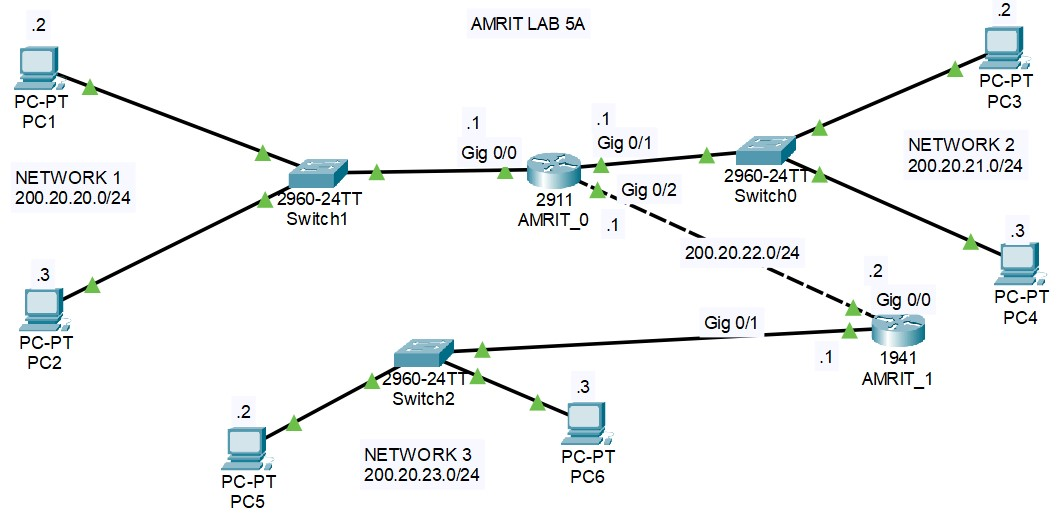
\includegraphics[scale=0.8,cframe=blue 0.5pt 3pt]{Lab5A.jpg}
    \caption{Network topology Lab 5A}
\end{figure}
\begin{enumerate}
    %%%%%%%%%%%%%%%%%%%%%%AAAAAAAAAAAAAAAAAAAAAAAAAAAAAAAA11111111111111111111111111
    \item\textbf{ Set the IP address of different computers as following:}

          \begin{itemize}


              \item PC1: \quad \quad 200.20.20.2 \quad \quad 255.255.255.0
                    \begin{figure}[H]
                        \centering
                        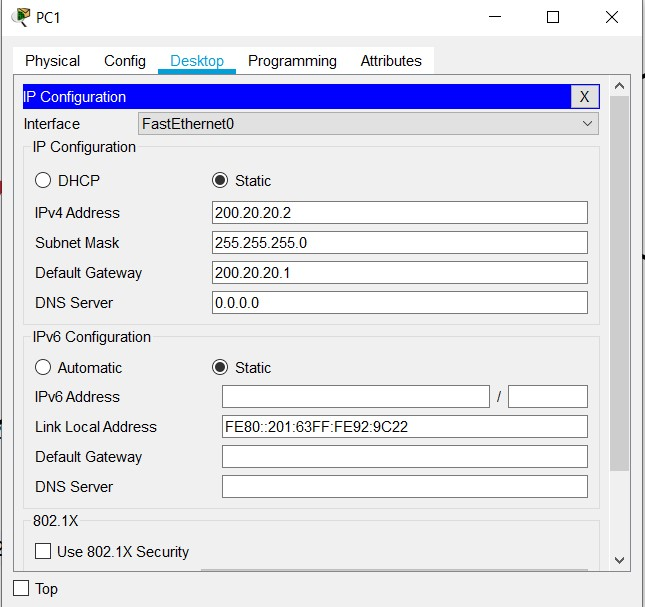
\includegraphics[scale=0.65,cframe=blue 0.5pt 3pt]{PC1 ip.jpg}
                        \caption{PC1 IP configuration}
                    \end{figure}

              \item PC2: \quad \quad 200.20.20.3 \quad \quad 255.255.255.0
              \item PC3: \quad \quad 200.20.21.2 \quad \quad 255.255.255.0
              \item PC4: \quad \quad 200.20.21.3 \quad \quad 255.255.255.0
              \item PC5: \quad \quad 200.20.23.2 \quad \quad 255.255.255.0
              \item PC6: \quad \quad 200.20.23.3 \quad \quad 255.255.255.0
          \end{itemize}

          Also set each of PCs with appropriate default gateway.\\
          Set the IP address of Router interfaces as:
          \begin{itemize}
              \item \textbf{Router 0:}
                    \begin{itemize}
                        \item GigabitEthernet 0/0: \quad \quad 200.20.20.1 \quad \quad 255.255.255.0
                              \addtocontents{lol}{\protect\subsection*{\HRule \\ Activities A\\ \HRule}}
                              \addtocontents{lol}{\protect\subsubsection*{A.1: Assign IP to Interfaces}}
                              \CMD{IP00.txt}{Assign the IP address of GigabitEthernet 0/0 for Router 0}

                        \item GigabitEthernet 0/1: \quad \quad 200.20.21.1 \quad \quad 255.255.255.0

                        \item GigabitEthernet 0/2: \quad \quad 200.20.22.1 \quad \quad 255.255.255.0\\

                    \end{itemize}


              \item \textbf{Router 1:}
                    \begin{itemize}
                        \item GigabitEthernet 0/0: \quad \quad 200.20.22.2 \quad \quad 255.255.255.0
                              \CMD{IP10.txt}{Assign the IP address of GigabitEthernet 0/0 for Router 1}

                        \item GigabitEthernet 0/1: \quad \quad 200.20.23.1 \quad \quad 255.255.255.0\\

                    \end{itemize}
          \end{itemize}


          \addtocontents{lot}{\protect\subsection*{\HRule \\ Activities A\\ \HRule}}
          \addtocontents{lot}{\protect\subsubsection*{A.1: Assign IP to Interfaces}}
          \begin{table}[H]
              \centering

              \begin{tabular}{| m{15em}| m{12em}|}
                  \hline
                  \rowcolor[rgb]{0.369,0.647,0.847} \textbf{Name} & \textbf{Assigned IP} \\
                  \hline
                  \textbf{PC1}                                    & 200.20.20.2          \\
                  \hline
                  \textbf{PC2}                                    & 200.20.20.3          \\
                  \hline
                  \textbf{Router 0 : 0/0}                         & 200.20.20.1          \\
                  \hline
                  \textbf{Router 0 : 0/1}                         & 200.20.21.1          \\
                  \hline
                  \textbf{Router 0 : 0/2}                         & 200.20.22.1          \\
                  \hline
                  \textbf{PC3}                                    & 200.20.21.2          \\
                  \hline
                  \textbf{PC4}                                    & 200.20.21.3          \\
                  \hline
                  \textbf{Router 1 : 0/0}                         & 200.20.22.2          \\
                  \hline
                  \textbf{Router 1 : 0/1}                         & 200.20.23.1          \\
                  \hline
                  \textbf{PC5}                                    & 200.20.23.2          \\
                  \hline
                  \textbf{PC6}                                    & 200.20.23.3          \\
                  \hline
              \end{tabular}
              \caption{Name and assigned IP Activity A}
          \end{table}


          %%%%%%%%%%%%%%%%%%%%%%AAAAAAAAAAAAAAAAAAAAAAAAAAAAAAAA22222222222222222222222
    \item\textbf{ Test the connectivity from PC2 to all other computers and all interfaces of Routers using ping and note down the result.}
          \addtocontents{lol}{\protect\subsubsection*{A.2: Ping from PC2}}
          \CMD{AP2-3.txt}{Ping from PC2 to PC3}

          \CMD{AP2-r11.txt}{Ping from PC2 to Router 1 : 0/1}

          % \usepackage{multirow}
          % \usepackage{colortbl}
          % \usepackage{hhline}

          \addtocontents{lot}{\protect\subsubsection*{A.2: Ping from PC2}}
          \begin{table}[H]
              \centering

              \arrayrulecolor{black}
              \begin{tabular}{| m{10em}| m{15em}| m{10em} |}
                  \hline
                  \multicolumn{1}{|l|}{\textbf{Sending Host}}                     & \textbf{Destination} & \multicolumn{1}{l|}{\textbf{Ping Status}}                             \\
                  \hline
                  {\cellcolor[rgb]{0.141,0.525,1}}                                & PC1                  & {\cellcolor[rgb]{0.404,1,0.835}}                                      \\
                  \hhline{|>{\arrayrulecolor[rgb]{0.141,0.525,1}}->{\arrayrulecolor{black}}->{\arrayrulecolor[rgb]{0.404,1,0.835}}->{\arrayrulecolor{black}}|}
                  {\cellcolor[rgb]{0.141,0.525,1}}                                & Router 0 : 0/0       & {\cellcolor[rgb]{0.404,1,0.835}}                                      \\
                  \hhline{|>{\arrayrulecolor[rgb]{0.141,0.525,1}}->{\arrayrulecolor{black}}->{\arrayrulecolor[rgb]{0.404,1,0.835}}->{\arrayrulecolor{black}}|}
                  {\cellcolor[rgb]{0.141,0.525,1}}                                & Router 0 : 0/1       & {\cellcolor[rgb]{0.404,1,0.835}}                                      \\
                  \hhline{|>{\arrayrulecolor[rgb]{0.141,0.525,1}}->{\arrayrulecolor{black}}->{\arrayrulecolor[rgb]{0.404,1,0.835}}->{\arrayrulecolor{black}}|}
                  {\cellcolor[rgb]{0.141,0.525,1}}                                & Router 0 : 0/2       & {\cellcolor[rgb]{0.404,1,0.835}}                                      \\
                  \hhline{|>{\arrayrulecolor[rgb]{0.141,0.525,1}}->{\arrayrulecolor{black}}->{\arrayrulecolor[rgb]{0.404,1,0.835}}->{\arrayrulecolor{black}}|}
                  {\cellcolor[rgb]{0.141,0.525,1}}                                & PC3                  & {\cellcolor[rgb]{0.404,1,0.835}}                                      \\
                  \hhline{|>{\arrayrulecolor[rgb]{0.141,0.525,1}}->{\arrayrulecolor{black}}->{\arrayrulecolor[rgb]{0.404,1,0.835}}->{\arrayrulecolor{black}}|}
                  {\cellcolor[rgb]{0.141,0.525,1}}                                & PC4                  & \multirow{-6}{*}{{\cellcolor[rgb]{0.404,1,0.835}}\textbf{Successful}} \\
                  \hhline{|>{\arrayrulecolor[rgb]{0.141,0.525,1}}->{\arrayrulecolor{black}}--|}
                  {\cellcolor[rgb]{0.141,0.525,1}}                                & Router 1 : 0/0       & {\cellcolor[rgb]{1,0.165,0.078}}                                      \\
                  \hhline{|>{\arrayrulecolor[rgb]{0.141,0.525,1}}->{\arrayrulecolor{black}}->{\arrayrulecolor[rgb]{1,0.165,0.078}}->{\arrayrulecolor{black}}|}
                  {\cellcolor[rgb]{0.141,0.525,1}}                                & Router 1 : 0/1       & {\cellcolor[rgb]{1,0.165,0.078}}                                      \\
                  \hhline{|>{\arrayrulecolor[rgb]{0.141,0.525,1}}->{\arrayrulecolor{black}}->{\arrayrulecolor[rgb]{1,0.165,0.078}}->{\arrayrulecolor{black}}|}
                  {\cellcolor[rgb]{0.141,0.525,1}}                                & PC5                  & {\cellcolor[rgb]{1,0.165,0.078}}                                      \\
                  \hhline{|>{\arrayrulecolor[rgb]{0.141,0.525,1}}->{\arrayrulecolor{black}}->{\arrayrulecolor[rgb]{1,0.165,0.078}}->{\arrayrulecolor{black}}|}
                  \multirow{-10}{*}{{\cellcolor[rgb]{0.141,0.525,1}}\textbf{PC2}} & PC6                  & \multirow{-4}{*}{{\cellcolor[rgb]{1,0.165,0.078}}\textbf{Failed}}     \\
                  \hline
              \end{tabular}
              \caption{Ping Status PC2 to all others}
          \end{table}




          %%%%%%%%%%%%%%%%%%%%%%AAAAAAAAAAAAAAAAAAAAAAAAAAAAAAAA3333333333333333333333333333
    \item\textbf{ Similarly test the connectivity from PC4 to all other computers and all interfaces of Routers using ping and note down the result.}
          \addtocontents{lol}{\protect\subsubsection*{A.3: Ping from PC4}}
          \CMD{AP4-2.txt}{Ping from PC4 to PC2}

          \CMD{AP4-r11.txt}{Ping from PC4 to Router 1 : 0/1}

          % \usepackage{multirow}
          % \usepackage{colortbl}
          % \usepackage{hhline}

          \addtocontents{lot}{\protect\subsubsection*{A.3: Ping from PC4}}
          \begin{table}[H]
              \centering

              \arrayrulecolor{black}
              \begin{tabular}{| m{10em}| m{10em}| m{10em} |}
                  \hline
                  \multicolumn{1}{|l|}{\textbf{Sending Host}}                     & \textbf{Destination} & \multicolumn{1}{l|}{\textbf{Ping Status}}                             \\
                  \hline
                  {\cellcolor[rgb]{0.141,0.525,1}}                                & PC1                  & {\cellcolor[rgb]{0.404,1,0.835}}                                      \\
                  \hhline{|>{\arrayrulecolor[rgb]{0.141,0.525,1}}->{\arrayrulecolor{black}}->{\arrayrulecolor[rgb]{0.404,1,0.835}}->{\arrayrulecolor{black}}|}
                  {\cellcolor[rgb]{0.141,0.525,1}}                                & PC2                  & {\cellcolor[rgb]{0.404,1,0.835}}                                      \\
                  \hhline{|>{\arrayrulecolor[rgb]{0.141,0.525,1}}->{\arrayrulecolor{black}}->{\arrayrulecolor[rgb]{0.404,1,0.835}}->{\arrayrulecolor{black}}|}
                  {\cellcolor[rgb]{0.141,0.525,1}}                                & Router 0 : 0/0       & {\cellcolor[rgb]{0.404,1,0.835}}                                      \\
                  \hhline{|>{\arrayrulecolor[rgb]{0.141,0.525,1}}->{\arrayrulecolor{black}}->{\arrayrulecolor[rgb]{0.404,1,0.835}}->{\arrayrulecolor{black}}|}
                  {\cellcolor[rgb]{0.141,0.525,1}}                                & Router 0 : 0/1       & {\cellcolor[rgb]{0.404,1,0.835}}                                      \\
                  \hhline{|>{\arrayrulecolor[rgb]{0.141,0.525,1}}->{\arrayrulecolor{black}}->{\arrayrulecolor[rgb]{0.404,1,0.835}}->{\arrayrulecolor{black}}|}
                  {\cellcolor[rgb]{0.141,0.525,1}}                                & Router 0 : 0/2       & {\cellcolor[rgb]{0.404,1,0.835}}                                      \\
                  \hhline{|>{\arrayrulecolor[rgb]{0.141,0.525,1}}->{\arrayrulecolor{black}}->{\arrayrulecolor[rgb]{0.404,1,0.835}}->{\arrayrulecolor{black}}|}
                  {\cellcolor[rgb]{0.141,0.525,1}}                                & PC3                  & \multirow{-6}{*}{{\cellcolor[rgb]{0.404,1,0.835}}\textbf{Successful}} \\
                  \hhline{|>{\arrayrulecolor[rgb]{0.141,0.525,1}}->{\arrayrulecolor{black}}--|}
                  {\cellcolor[rgb]{0.141,0.525,1}}                                & Router 1 : 0/0       & {\cellcolor[rgb]{1,0.165,0.078}}                                      \\
                  \hhline{|>{\arrayrulecolor[rgb]{0.141,0.525,1}}->{\arrayrulecolor{black}}->{\arrayrulecolor[rgb]{1,0.165,0.078}}->{\arrayrulecolor{black}}|}
                  {\cellcolor[rgb]{0.141,0.525,1}}                                & Router 1 : 0/1       & {\cellcolor[rgb]{1,0.165,0.078}}                                      \\
                  \hhline{|>{\arrayrulecolor[rgb]{0.141,0.525,1}}->{\arrayrulecolor{black}}->{\arrayrulecolor[rgb]{1,0.165,0.078}}->{\arrayrulecolor{black}}|}
                  {\cellcolor[rgb]{0.141,0.525,1}}                                & PC5                  & {\cellcolor[rgb]{1,0.165,0.078}}                                      \\
                  \hhline{|>{\arrayrulecolor[rgb]{0.141,0.525,1}}->{\arrayrulecolor{black}}->{\arrayrulecolor[rgb]{1,0.165,0.078}}->{\arrayrulecolor{black}}|}
                  \multirow{-10}{*}{{\cellcolor[rgb]{0.141,0.525,1}}\textbf{PC4}} & PC6                  & \multirow{-4}{*}{{\cellcolor[rgb]{1,0.165,0.078}}\textbf{Failed}}     \\
                  \hline
              \end{tabular}
              \caption{ Ping Status PC4 to all others}
          \end{table}



          %%%%%%%%%%%%%%%%%%%%%%AAAAAAAAAAAAAAAAAAAAAAAAAAAAAAAA4444444444444444444444444444
    \item\textbf{ Similarly test the connectivity from PC6 to all other computers and all interfaces of Routers using ping and note down the result.}
          \addtocontents{lol}{\protect\subsubsection*{A.4 :Ping from PC6}}
          \CMD{AP6-2.txt}{Ping from PC6 to PC2}

          \CMD{AP6-r01.txt}{Ping from PC6 to Router 0 : 0/1}


          \addtocontents{lot}{\protect\subsubsection*{A.4 :Ping from PC6}}
          \begin{table}[H]
              \centering

              \arrayrulecolor{black}
              \begin{tabular}{| m{10em}| m{10em}| m{10em} |}
                  \hline
                  \multicolumn{1}{|l|}{\textbf{Sending Host}}                     & \textbf{Destination} & \multicolumn{1}{l|}{\textbf{Ping Status}}                                 \\
                  \hline
                  {\cellcolor[rgb]{0.141,0.525,1}}                                & PC1                  & {\cellcolor[rgb]{1,0.169,0.082}}                                          \\
                  \hhline{|>{\arrayrulecolor[rgb]{0.141,0.525,1}}->{\arrayrulecolor{black}}->{\arrayrulecolor[rgb]{1,0.169,0.082}}->{\arrayrulecolor{black}}|}
                  {\cellcolor[rgb]{0.141,0.525,1}}                                & PC2                  & {\cellcolor[rgb]{1,0.169,0.082}}                                          \\
                  \hhline{|>{\arrayrulecolor[rgb]{0.141,0.525,1}}->{\arrayrulecolor{black}}->{\arrayrulecolor[rgb]{1,0.169,0.082}}->{\arrayrulecolor{black}}|}
                  {\cellcolor[rgb]{0.141,0.525,1}}                                & Router 0 : 0/0       & {\cellcolor[rgb]{1,0.169,0.082}}                                          \\
                  \hhline{|>{\arrayrulecolor[rgb]{0.141,0.525,1}}->{\arrayrulecolor{black}}->{\arrayrulecolor[rgb]{1,0.169,0.082}}->{\arrayrulecolor{black}}|}
                  {\cellcolor[rgb]{0.141,0.525,1}}                                & Router 0 : 0/1       & {\cellcolor[rgb]{1,0.169,0.082}}                                          \\
                  \hhline{|>{\arrayrulecolor[rgb]{0.141,0.525,1}}->{\arrayrulecolor{black}}->{\arrayrulecolor[rgb]{1,0.169,0.082}}->{\arrayrulecolor{black}}|}
                  {\cellcolor[rgb]{0.141,0.525,1}}                                & Router 0 : 0/2       & {\cellcolor[rgb]{1,0.169,0.082}}                                          \\
                  \hhline{|>{\arrayrulecolor[rgb]{0.141,0.525,1}}->{\arrayrulecolor{black}}->{\arrayrulecolor[rgb]{1,0.169,0.082}}->{\arrayrulecolor{black}}|}
                  {\cellcolor[rgb]{0.141,0.525,1}}                                & PC3                  & {\cellcolor[rgb]{1,0.169,0.082}}                                          \\
                  \hhline{|>{\arrayrulecolor[rgb]{0.141,0.525,1}}->{\arrayrulecolor{black}}->{\arrayrulecolor[rgb]{1,0.169,0.082}}->{\arrayrulecolor{black}}|}
                  {\cellcolor[rgb]{0.141,0.525,1}}                                & PC4                  & \multirow{-7}{*}{{\cellcolor[rgb]{1,0.169,0.082}}\textbf{Failed}}         \\
                  \hhline{|>{\arrayrulecolor[rgb]{0.141,0.525,1}}->{\arrayrulecolor{black}}--|}
                  {\cellcolor[rgb]{0.141,0.525,1}}                                & Router 1 : 0/0       & {\cellcolor[rgb]{0.396,0.984,0.804}}                                      \\
                  \hhline{|>{\arrayrulecolor[rgb]{0.141,0.525,1}}->{\arrayrulecolor{black}}->{\arrayrulecolor[rgb]{0.396,0.984,0.804}}->{\arrayrulecolor{black}}|}
                  {\cellcolor[rgb]{0.141,0.525,1}}                                & Router 1 : 0/1       & {\cellcolor[rgb]{0.396,0.984,0.804}}                                      \\
                  \hhline{|>{\arrayrulecolor[rgb]{0.141,0.525,1}}->{\arrayrulecolor{black}}->{\arrayrulecolor[rgb]{0.396,0.984,0.804}}->{\arrayrulecolor{black}}|}
                  \multirow{-10}{*}{{\cellcolor[rgb]{0.141,0.525,1}}\textbf{PC6}} & PC5                  & \multirow{-3}{*}{{\cellcolor[rgb]{0.396,0.984,0.804}}\textbf{Successful}} \\
                  \hline
              \end{tabular}
              \caption{ Ping Status PC6 to all others}
          \end{table}




          %%%%%%%%%%%%%%%%%%%%%%AAAAAAAAAAAAAAAAAAAAAAAAAAAAAAAA55555555555555555555555
    \item\textbf{ Use default route configuration in each Router to forward the network traffic to another  Router and observe the output of \textit{show ip route} command in both Routers}
          \addtocontents{lol}{\protect\subsubsection*{A.5: Default Route Configuration}}
          \CMD{A_default route 0.txt}{Default Route configuration in Router 0}
          \CMD{A_Showip0.txt}{\textit{show ip route} Router 0}

          \CMD{A_default route 1.txt}{Default Route configuration in Router 1}
          \CMD{A_Showip1.txt}{\textit{show ip route} Router 1}

          Here default route is configured in such a way that all unknown destination request and packets are forwarded to next Router available. For example in Router 0 all packets meant for Network 3 is forwarded to Router 1's GigabitEthernet 0/0.

          %%%%%%%%%%%%%%%%%%%%%%AAAAAAAAAAAAAAAAAAAAAAAAAAAAAAAA6666666666666666666
    \item\textbf{ Again test connectivity by repeating step 2 to 4 and note down the result. Compare this observation with previous and comment on the result.}

          \begin{itemize}
              \item \textbf{Test the connectivity from PC2 to all other computers and all interfaces of Routers using ping
                        and note down the result.}
                    \addtocontents{lol}{\protect\subsubsection*{A.6: Repeating A.2 to A.4 After Default Route Configuration}}
                    \CMD{DAP2-6.txt}{Ping from PC2 to PC6 after Default Configuration}

                    % \usepackage{multirow}
                    % \usepackage{colortbl}
                    % \usepackage{hhline}

                    \addtocontents{lot}{\protect\subsubsection*{A.6: Repeating A.2 to A.4 After Default Route Configuration}}
                    \begin{table}[H]
                        \centering

                        \arrayrulecolor{black}
                        \begin{tabular}{| m{10em}| m{10em}| m{10em} |}
                            \hline
                            \multicolumn{1}{|l|}{\textbf{Sending Host}}                     & \textbf{Destination} & \multicolumn{1}{l|}{\textbf{Ping Status}}                                  \\
                            \hline
                            {\cellcolor[rgb]{0.141,0.525,1}}                                & PC1                  & {\cellcolor[rgb]{0.42,0.988,0.827}}                                        \\
                            \hhline{|>{\arrayrulecolor[rgb]{0.141,0.525,1}}->{\arrayrulecolor{black}}->{\arrayrulecolor[rgb]{0.42,0.988,0.827}}->{\arrayrulecolor{black}}|}
                            {\cellcolor[rgb]{0.141,0.525,1}}                                & Router 0 : 0/0       & {\cellcolor[rgb]{0.42,0.988,0.827}}                                        \\
                            \hhline{|>{\arrayrulecolor[rgb]{0.141,0.525,1}}->{\arrayrulecolor{black}}->{\arrayrulecolor[rgb]{0.42,0.988,0.827}}->{\arrayrulecolor{black}}|}
                            {\cellcolor[rgb]{0.141,0.525,1}}                                & Router 0 : 0/1       & {\cellcolor[rgb]{0.42,0.988,0.827}}                                        \\
                            \hhline{|>{\arrayrulecolor[rgb]{0.141,0.525,1}}->{\arrayrulecolor{black}}->{\arrayrulecolor[rgb]{0.42,0.988,0.827}}->{\arrayrulecolor{black}}|}
                            {\cellcolor[rgb]{0.141,0.525,1}}                                & Router 0 : 0/2       & {\cellcolor[rgb]{0.42,0.988,0.827}}                                        \\
                            \hhline{|>{\arrayrulecolor[rgb]{0.141,0.525,1}}->{\arrayrulecolor{black}}->{\arrayrulecolor[rgb]{0.42,0.988,0.827}}->{\arrayrulecolor{black}}|}
                            {\cellcolor[rgb]{0.141,0.525,1}}                                & PC3                  & {\cellcolor[rgb]{0.42,0.988,0.827}}                                        \\
                            \hhline{|>{\arrayrulecolor[rgb]{0.141,0.525,1}}->{\arrayrulecolor{black}}->{\arrayrulecolor[rgb]{0.42,0.988,0.827}}->{\arrayrulecolor{black}}|}
                            {\cellcolor[rgb]{0.141,0.525,1}}                                & PC4                  & {\cellcolor[rgb]{0.42,0.988,0.827}}                                        \\
                            \hhline{|>{\arrayrulecolor[rgb]{0.141,0.525,1}}->{\arrayrulecolor{black}}->{\arrayrulecolor[rgb]{0.42,0.988,0.827}}->{\arrayrulecolor{black}}|}
                            {\cellcolor[rgb]{0.141,0.525,1}}                                & Router 1 : 0/0       & {\cellcolor[rgb]{0.42,0.988,0.827}}                                        \\
                            \hhline{|>{\arrayrulecolor[rgb]{0.141,0.525,1}}->{\arrayrulecolor{black}}->{\arrayrulecolor[rgb]{0.42,0.988,0.827}}->{\arrayrulecolor{black}}|}
                            {\cellcolor[rgb]{0.141,0.525,1}}                                & Router 1 : 0/1       & {\cellcolor[rgb]{0.42,0.988,0.827}}                                        \\
                            \hhline{|>{\arrayrulecolor[rgb]{0.141,0.525,1}}->{\arrayrulecolor{black}}->{\arrayrulecolor[rgb]{0.42,0.988,0.827}}->{\arrayrulecolor{black}}|}
                            {\cellcolor[rgb]{0.141,0.525,1}}                                & PC5                  & {\cellcolor[rgb]{0.42,0.988,0.827}}                                        \\
                            \hhline{|>{\arrayrulecolor[rgb]{0.141,0.525,1}}->{\arrayrulecolor{black}}->{\arrayrulecolor[rgb]{0.42,0.988,0.827}}->{\arrayrulecolor{black}}|}
                            \multirow{-10}{*}{{\cellcolor[rgb]{0.141,0.525,1}}\textbf{PC2}} & PC6                  & \multirow{-10}{*}{{\cellcolor[rgb]{0.42,0.988,0.827}} \textbf{Successful}} \\
                            \hline
                        \end{tabular}
                        \caption{ Ping Status PC2 to all others after Default route Configuration}
                    \end{table}

                    Previously Ping operation was Successful to its network or only to Network connected to  Router 0 and  Ping failed when PC2 tries to ping Router and PCs of Network 3 and all packet forwarded to Network 3 is dropped and error message is sent back to host. But after default route is set in both Routers, Router 0 forward all the packets to Router 1 if there is no entries of destination network in its routing Table. So, the packets reached its destination network i.e Network 3 and ping is successful.

              \item \textbf{Similarly test the connectivity from PC4 to all other computers and all interfaces of Routers
                        using ping and note down the result.}

                    \CMD{DAP4-6.txt}{Ping from PC4 to PC6 after Default Configuration}

                    % \usepackage{multirow}
                    % \usepackage{colortbl}
                    % \usepackage{hhline}


                    \begin{table}[H]
                        \centering

                        \arrayrulecolor{black}
                        \begin{tabular}{| m{10em}| m{10em}| m{10em} |}
                            \hline
                            \multicolumn{1}{|l|}{\textbf{Sending Host}}                     & \textbf{Destination} & \multicolumn{1}{l|}{\textbf{Ping Status}}                                  \\
                            \hline
                            {\cellcolor[rgb]{0.141,0.525,1}}                                & PC1                  & {\cellcolor[rgb]{0.42,0.988,0.827}}                                        \\
                            \hhline{|>{\arrayrulecolor[rgb]{0.141,0.525,1}}->{\arrayrulecolor{black}}->{\arrayrulecolor[rgb]{0.42,0.988,0.827}}->{\arrayrulecolor{black}}|}
                            {\cellcolor[rgb]{0.141,0.525,1}}                                & PC2                  & {\cellcolor[rgb]{0.42,0.988,0.827}}                                        \\
                            \hhline{|>{\arrayrulecolor[rgb]{0.141,0.525,1}}->{\arrayrulecolor{black}}->{\arrayrulecolor[rgb]{0.42,0.988,0.827}}->{\arrayrulecolor{black}}|}
                            {\cellcolor[rgb]{0.141,0.525,1}}                                & Router 0 : 0/0       & {\cellcolor[rgb]{0.42,0.988,0.827}}                                        \\
                            \hhline{|>{\arrayrulecolor[rgb]{0.141,0.525,1}}->{\arrayrulecolor{black}}->{\arrayrulecolor[rgb]{0.42,0.988,0.827}}->{\arrayrulecolor{black}}|}
                            {\cellcolor[rgb]{0.141,0.525,1}}                                & Router 0 : 0/1       & {\cellcolor[rgb]{0.42,0.988,0.827}}                                        \\
                            \hhline{|>{\arrayrulecolor[rgb]{0.141,0.525,1}}->{\arrayrulecolor{black}}->{\arrayrulecolor[rgb]{0.42,0.988,0.827}}->{\arrayrulecolor{black}}|}
                            {\cellcolor[rgb]{0.141,0.525,1}}                                & Router 0 : 0/2       & {\cellcolor[rgb]{0.42,0.988,0.827}}                                        \\
                            \hhline{|>{\arrayrulecolor[rgb]{0.141,0.525,1}}->{\arrayrulecolor{black}}->{\arrayrulecolor[rgb]{0.42,0.988,0.827}}->{\arrayrulecolor{black}}|}
                            {\cellcolor[rgb]{0.141,0.525,1}}                                & PC3                  & {\cellcolor[rgb]{0.42,0.988,0.827}}                                        \\
                            \hhline{|>{\arrayrulecolor[rgb]{0.141,0.525,1}}->{\arrayrulecolor{black}}->{\arrayrulecolor[rgb]{0.42,0.988,0.827}}->{\arrayrulecolor{black}}|}
                            {\cellcolor[rgb]{0.141,0.525,1}}                                & Router 1 : 0/0       & {\cellcolor[rgb]{0.42,0.988,0.827}}                                        \\
                            \hhline{|>{\arrayrulecolor[rgb]{0.141,0.525,1}}->{\arrayrulecolor{black}}->{\arrayrulecolor[rgb]{0.42,0.988,0.827}}->{\arrayrulecolor{black}}|}
                            {\cellcolor[rgb]{0.141,0.525,1}}                                & Router 1 : 0/1       & {\cellcolor[rgb]{0.42,0.988,0.827}}                                        \\
                            \hhline{|>{\arrayrulecolor[rgb]{0.141,0.525,1}}->{\arrayrulecolor{black}}->{\arrayrulecolor[rgb]{0.42,0.988,0.827}}->{\arrayrulecolor{black}}|}
                            {\cellcolor[rgb]{0.141,0.525,1}}                                & PC5                  & {\cellcolor[rgb]{0.42,0.988,0.827}}                                        \\
                            \hhline{|>{\arrayrulecolor[rgb]{0.141,0.525,1}}->{\arrayrulecolor{black}}->{\arrayrulecolor[rgb]{0.42,0.988,0.827}}->{\arrayrulecolor{black}}|}
                            \multirow{-10}{*}{{\cellcolor[rgb]{0.141,0.525,1}}\textbf{PC4}} & PC6                  & \multirow{-10}{*}{{\cellcolor[rgb]{0.42,0.988,0.827}} \textbf{Successful}} \\
                            \hline
                        \end{tabular}
                        \caption{ Ping Status PC4 to all others after Default route Configuration}
                    \end{table}

                    Previously Ping operation was Successful to its network or only to Network connected to  Router 0 and  Ping failed when PC4 tries to ping Router and PCs of Network 3 and all packet forwarded to Network 3 is dropped and error message is sent back to host. But after default route is set in both Routers, Router 0 forward all the packets to Router 1 if there is no entries of destination network in its routing Table. So, the packets reached its destination network i.e Network 3 and ping is successful.


              \item \textbf{Similarly test the connectivity from PC6 to all other computers and all interfaces of Routers
                        using ping and note down the result.}

                    \CMD{DAP6-2.txt}{Ping from PC6 to PC2 after Default Configuration}
                    % \usepackage{multirow}
                    % \usepackage{colortbl}
                    % \usepackage{hhline}


                    \begin{table}[H]
                        \centering
                        \arrayrulecolor{black}
                        \begin{tabular}{| m{10em}| m{10em}| m{10em} |}
                            \hline
                            \multicolumn{1}{|l|}{\textbf{Sending Host}}                     & \textbf{Destination} & \multicolumn{1}{l|}{\textbf{Ping Status}}                                  \\
                            \hline
                            {\cellcolor[rgb]{0.141,0.525,1}}                                & PC1                  & {\cellcolor[rgb]{0.42,0.988,0.827}}                                        \\
                            \hhline{|>{\arrayrulecolor[rgb]{0.141,0.525,1}}->{\arrayrulecolor{black}}->{\arrayrulecolor[rgb]{0.42,0.988,0.827}}->{\arrayrulecolor{black}}|}
                            {\cellcolor[rgb]{0.141,0.525,1}}                                & PC2                  & {\cellcolor[rgb]{0.42,0.988,0.827}}                                        \\
                            \hhline{|>{\arrayrulecolor[rgb]{0.141,0.525,1}}->{\arrayrulecolor{black}}->{\arrayrulecolor[rgb]{0.42,0.988,0.827}}->{\arrayrulecolor{black}}|}
                            {\cellcolor[rgb]{0.141,0.525,1}}                                & Router 0 : 0/0       & {\cellcolor[rgb]{0.42,0.988,0.827}}                                        \\
                            \hhline{|>{\arrayrulecolor[rgb]{0.141,0.525,1}}->{\arrayrulecolor{black}}->{\arrayrulecolor[rgb]{0.42,0.988,0.827}}->{\arrayrulecolor{black}}|}
                            {\cellcolor[rgb]{0.141,0.525,1}}                                & Router 0 : 0/1       & {\cellcolor[rgb]{0.42,0.988,0.827}}                                        \\
                            \hhline{|>{\arrayrulecolor[rgb]{0.141,0.525,1}}->{\arrayrulecolor{black}}->{\arrayrulecolor[rgb]{0.42,0.988,0.827}}->{\arrayrulecolor{black}}|}
                            {\cellcolor[rgb]{0.141,0.525,1}}                                & Router 0 : 0/2       & {\cellcolor[rgb]{0.42,0.988,0.827}}                                        \\
                            \hhline{|>{\arrayrulecolor[rgb]{0.141,0.525,1}}->{\arrayrulecolor{black}}->{\arrayrulecolor[rgb]{0.42,0.988,0.827}}->{\arrayrulecolor{black}}|}
                            {\cellcolor[rgb]{0.141,0.525,1}}                                & PC3                  & {\cellcolor[rgb]{0.42,0.988,0.827}}                                        \\
                            \hhline{|>{\arrayrulecolor[rgb]{0.141,0.525,1}}->{\arrayrulecolor{black}}->{\arrayrulecolor[rgb]{0.42,0.988,0.827}}->{\arrayrulecolor{black}}|}
                            {\cellcolor[rgb]{0.141,0.525,1}}                                & PC4                  & {\cellcolor[rgb]{0.42,0.988,0.827}}                                        \\
                            \hhline{|>{\arrayrulecolor[rgb]{0.141,0.525,1}}->{\arrayrulecolor{black}}->{\arrayrulecolor[rgb]{0.42,0.988,0.827}}->{\arrayrulecolor{black}}|}
                            {\cellcolor[rgb]{0.141,0.525,1}}                                & Router 1 : 0/0       & {\cellcolor[rgb]{0.42,0.988,0.827}}                                        \\
                            \hhline{|>{\arrayrulecolor[rgb]{0.141,0.525,1}}->{\arrayrulecolor{black}}->{\arrayrulecolor[rgb]{0.42,0.988,0.827}}->{\arrayrulecolor{black}}|}
                            {\cellcolor[rgb]{0.141,0.525,1}}                                & Router 1 : 0/1       & {\cellcolor[rgb]{0.42,0.988,0.827}}                                        \\
                            \hhline{|>{\arrayrulecolor[rgb]{0.141,0.525,1}}->{\arrayrulecolor{black}}->{\arrayrulecolor[rgb]{0.42,0.988,0.827}}->{\arrayrulecolor{black}}|}
                            \multirow{-10}{*}{{\cellcolor[rgb]{0.141,0.525,1}}\textbf{PC6}} & PC5                  & \multirow{-10}{*}{{\cellcolor[rgb]{0.42,0.988,0.827}} \textbf{Successful}} \\
                            \hline
                        \end{tabular}
                        \caption{ Ping Status PC6 to all others after Default route Configuration}
                    \end{table}

                    Previously Ping operation was Successful to its network or only to Network connected to  Router 1 and  Ping failed when PC6 tries to ping Router and PCs of Network 1 or Network 2 and all packet forwarded to these Network are dropped and error message is sent back to host. But after default route is set in both Routers, Router 1 forward all the packets to Router 0 if there is no entries of destination network in its routing Table. So, the packets reached its destination network i.e Network 1 or Network 2 and ping is successful.

          \end{itemize}



          %%%%%%%%%%%%%%%%%%%%%%AAAAAAAAAAAAAAAAAAAAAAAAAAAAAAAA777777777777777777777
    \item\textbf{ Here the hostname of Router0 should be your FirstName\_0 and hostname of Router1 should be your FirstName\_1.}
          \addtocontents{lol}{\protect\subsubsection*{A.7: Set Hostname}}
          \CMD{Hostname_0.txt}{Setting Hostname for Router 0 to Amrit\_0}
          \CMD{Hostname_1.txt}{Setting Hostname for Router 1 to Amrit\_1}




\end{enumerate}




\pagebreak

%
%
%

%%%%%%%%%%%%%%%%%%%%%%%%%%%%%%BBBBBBBBBBBBBBBBBBBBBBBBB
%%%%%%%%%%%%%%%%%%%%%%%%%%%%%%BBBBBBBBBBBBBBBBBBBBBBBBB
%%%%%%%%%%%%%%%%%%%%%%%%%%%%%%BBBBBBBBBBBBBBBBBBBBBBBBB
%%%%%%%%%%%%%%%%%%%%%%%%%%%%%%BBBBBBBBBBBBBBBBBBBBBBBBB

%
%
%

\subsubsection{Activities B}

{\bfseries \textit{B. Create the following network topology and perform the followings:}}

\begin{figure}[H]
    \centering
    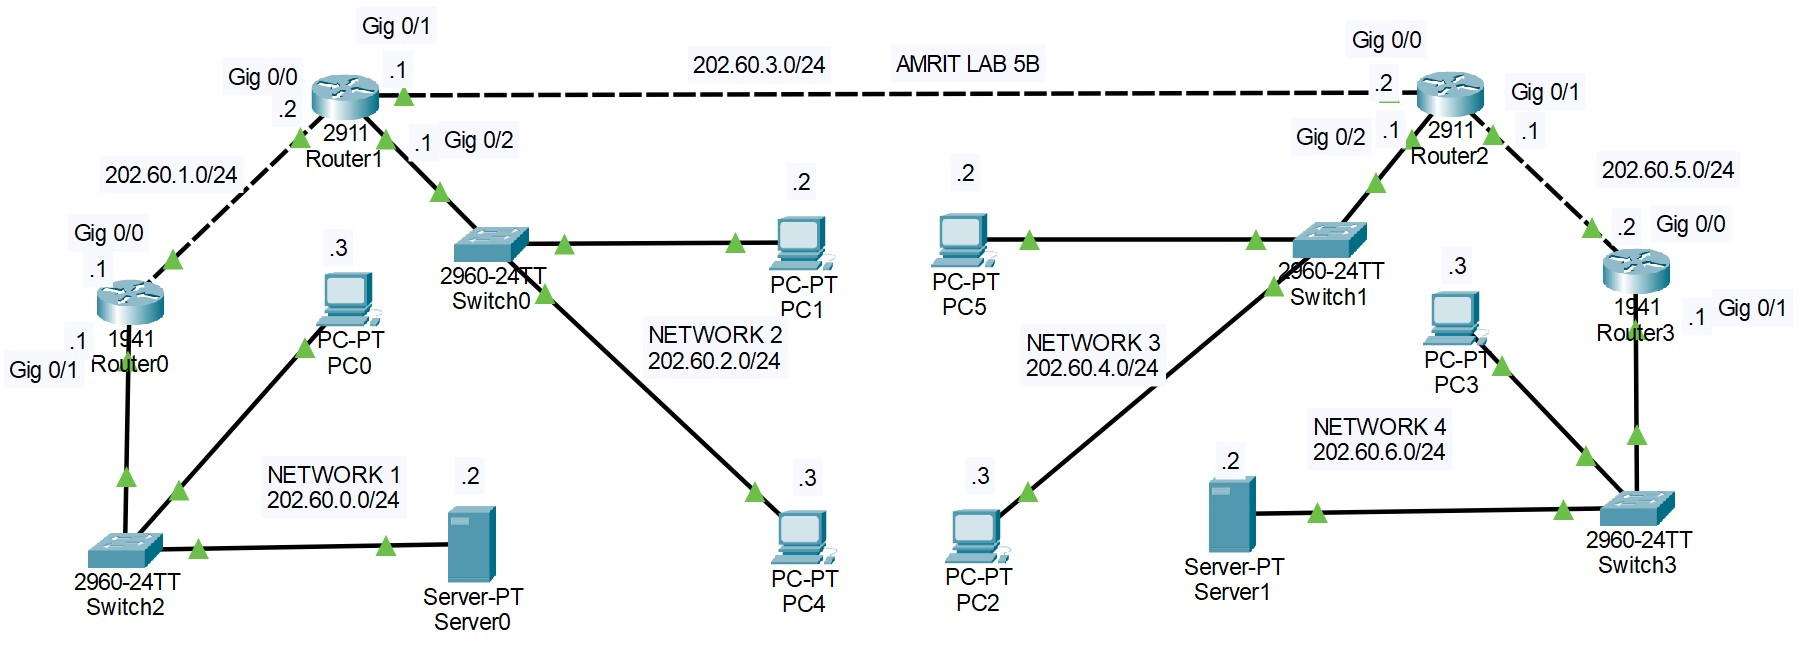
\includegraphics[scale=0.48,cframe=blue 0.5pt 3pt]{Lab5B.jpg}
    \caption{Network topology Lab 5B}
\end{figure}

\begin{enumerate}
    %%%%%%%%%%%%%%%%%%%%%%%%%%%%%%BBBBBBBBBBBBBBBBBBBBBBBBB11111111111111111111111
    \item\textbf{Configure the hostname, console password and enable password in each Router.}
          \addtocontents{lol}{\protect\subsection*{\HRule \\Activities B\\ \HRule}}
          \addtocontents{lol}{\protect\subsubsection*{B.1 : Routers Configuration}}
          \CMD{B_config0.txt}{Config Hostname, Console ,enable,vty password for Router 0}

          % \usepackage{colortbl}

          \addtocontents{lot}{\protect\subsection*{\HRule \\Activities B\\ \HRule}}
          \addtocontents{lot}{\protect\subsubsection*{B.1 : Routers Configuration}}

          \begin{table}[H]
              \centering
              \begin{tabular} {| m{6em}| m{6em}| m{9em} | m{8em}| m{7em} |}
                  \hline
                  {\cellcolor[rgb]{0.278,0.671,0.984}}\textbf{S.N} & \textbf{Hostname} & \textbf{Console Password} & \textbf{Enable Password} & \textbf{vty Password} \\
                  \hline
                  {\cellcolor[rgb]{0.278,0.671,0.984}}Router 0     & AMRIT\_0          & amrit                     & 403                      & phuyal                \\
                  \hline
                  {\cellcolor[rgb]{0.278,0.671,0.984}}Router 1     & AMRIT\_1          & amrit                     & 403                      & phuyal                \\
                  \hline
                  {\cellcolor[rgb]{0.278,0.671,0.984}}Router 2     & AMRIT\_2          & amrit                     & 403                      & phuyal                \\
                  \hline
                  {\cellcolor[rgb]{0.278,0.671,0.984}}Router 3     & AMRIT\_3          & amrit                     & 403                      & phuyal                \\
                  \hline
              \end{tabular}
              \caption{Table for hostname, console password , enable password,vty password}
          \end{table}


          %%%%%%%%%%%%%%%%%%%%%%%%%%%%%%BBBBBBBBBBBBBBBBBBBBBBBBB222222222222222222222222222
    \item\textbf{ Configure each interfaces of Router with given IP address and appropriate interface  description.}

          \addtocontents{lol}{\protect\subsubsection*{B.2 : Assign IP to Interfaces}}
          \CMD{B_IP0.txt}{Configuring each interface of Router0}
          \CMD{B_IP3.txt}{Configuring each interface of Router3}
          % \usepackage{colortbl}
          % \usepackage{multirow}
          % \usepackage{hhline}


          \addtocontents{lot}{\protect\subsubsection*{B.2 : Assign IP to Interfaces}}
          \begin{table}[H]
              \centering
              \
              \begin{tabular}{|l|l|l|l|}
                  \hline
                  \rowcolor[rgb]{0.443,0.831,1} \textbf{Router no.} & {\cellcolor[rgb]{0.325,1,0.784}}\textbf{GigabitEthernet} & \textbf{Assigned Ip} & \textbf{Description}    \\
                  \hline
                  \multirow{2}{*}{\textbf{Router 0~ }}              & {\cellcolor[rgb]{0.325,1,0.784}}0/0                      & 202.60.1.1           & Connected to Router 1~~ \\
                  \hhline{|~---|}
                                                                    & {\cellcolor[rgb]{0.325,1,0.784}}0/1                      & 202.60.0.1           & Connected to Network 1  \\
                  \hline
                  \multirow{3}{*}{\textbf{Router 1~~ }}             & {\cellcolor[rgb]{0.325,1,0.784}}0/0                      & 202.60.1.2           & Connected to Router 0   \\
                  \hhline{|~---|}
                                                                    & {\cellcolor[rgb]{0.325,1,0.784}}0/1                      & 202.60.3.1           & Connected to Router 2   \\
                  \hhline{|~---|}
                                                                    & {\cellcolor[rgb]{0.325,1,0.784}}0/2                      & 202.60.2.1           & Connected to Network 2  \\
                  \hline
                  \multirow{3}{*}{\textbf{~Router 2~~ }}            & {\cellcolor[rgb]{0.325,1,0.784}}0/0                      & 202.60.3.2           & Connected to Router 1   \\
                  \hhline{|~---|}
                                                                    & {\cellcolor[rgb]{0.325,1,0.784}}0/1                      & 202.60.5.1           & Connected to Router 3   \\
                  \hhline{|~---|}
                                                                    & {\cellcolor[rgb]{0.325,1,0.784}}0/2                      & 202.60.4.1           & Connected to Network 3  \\
                  \hline
                  \multirow{2}{*}{\textbf{Router 3 }}               & {\cellcolor[rgb]{0.325,1,0.784}}0/0                      & 202.60.5.2           & Connected to Router 2   \\
                  \hhline{|~---|}
                                                                    & {\cellcolor[rgb]{0.325,1,0.784}}0/1                      & 202.60.6.1           & Connected to Network 4  \\
                  \hline
              \end{tabular}
              \caption{Assigned IPs and description for all interfaces}
          \end{table}


          %%%%%%%%%%%%%%%%%%%%%%%%%%%%%%BBBBBBBBBBBBBBBBBBBBBBBBB3333333333333333333333333333333
    \item\textbf{ Configure the IP address and default gateway on each computer as specified in figure above. }

          % \usepackage{multirow}
          % \usepackage{colortbl}
          % \usepackage{hhline}

          \addtocontents{lot}{\protect\subsubsection*{B.3 : Configure the IP address and default gateway}}
          \begin{table}[H]
              \centering

              \arrayrulecolor{black}
              \begin{tabular}{| m{6em}| m{8em}| m{9em} | m{8em} |}
                  \hline
                  \rowcolor[rgb]{0.235,1,0.808} \textbf{Network no.~}         & \textbf{Default gateway}    & \textbf{~Device name} & \textbf{Assigned IP} \\
                  \hline
                  {\cellcolor[rgb]{0.259,0.753,1}}                            & \multirow{2}{*}{202.60.0.1} & Server 0              & 202.60.0.2           \\
                  \hhline{|>{\arrayrulecolor[rgb]{0.259,0.753,1}}-~>{\arrayrulecolor{black}}--|}
                  \multirow{-2}{*}{{\cellcolor[rgb]{0.259,0.753,1}}Network 1} &                             & PC0                   & 202.60.0.3           \\
                  \hline
                  {\cellcolor[rgb]{0.259,0.753,1}}                            & \multirow{2}{*}{202.60.2.1} & PC1                   & 202.60.2.2           \\
                  \hhline{|>{\arrayrulecolor[rgb]{0.259,0.753,1}}-~>{\arrayrulecolor{black}}--|}
                  \multirow{-2}{*}{{\cellcolor[rgb]{0.259,0.753,1}}Network 2} &                             & PC4                   & 202.60.2.3           \\
                  \hline
                  {\cellcolor[rgb]{0.259,0.753,1}}                            & \multirow{2}{*}{202.60.4.1} & PC5                   & 202.60.4.2           \\
                  \hhline{|>{\arrayrulecolor[rgb]{0.259,0.753,1}}-~>{\arrayrulecolor{black}}--|}
                  \multirow{-2}{*}{{\cellcolor[rgb]{0.259,0.753,1}}Network 3} &                             & PC2                   & 202.60.4.3           \\
                  \hline
                  {\cellcolor[rgb]{0.259,0.753,1}}                            & \multirow{2}{*}{202.60.6.1} & Server 1              & 202.60.6.2           \\
                  \hhline{|>{\arrayrulecolor[rgb]{0.259,0.753,1}}-~>{\arrayrulecolor{black}}--|}
                  \multirow{-2}{*}{{\cellcolor[rgb]{0.259,0.753,1}}Network 4} &                             & PC3                   & 202.60.6.3           \\
                  \hline
              \end{tabular}
              \caption{Table for Name, assigned ip, Default gateway}
          \end{table}

          %%%%%%%%%%%%%%%%%%%%%%%%%%%%%%BBBBBBBBBBBBBBBBBBBBBBBBB44444444444444444444444444444
    \item\textbf{ Enable telnet on each Router. }

          Already enabled in Activity B.1

          %%%%%%%%%%%%%%%%%%%%%%%%%%%%%%BBBBBBBBBBBBBBBBBBBBBBBBB55555555555555555555555555555
    \item\textbf{ Observe the output of the command \textit{show ip route} in each Router and note it down.}
          \addtocontents{lol}{\protect\subsubsection*{B.5 : Routing table of Routers}}
          \CMD{B_Showip0.txt}{\textit{show ip route} Router 0}
          \CMD{B_Showip1.txt}{\textit{show ip route} Router 1}
          \CMD{B_Showip2.txt}{\textit{show ip route} Router 2}
          \CMD{B_Showip3.txt}{\textit{show ip route} Router 3}

          %%%%%%%%%%%%%%%%%%%%%%%%%%%%%%BBBBBBBBBBBBBBBBBBBBBBBBB666666666666666666666666666
    \item\textbf{ Observe the output while using ping command from PC0 to PC0, PC1, PC2, PC3, Server0,
              Server1, Router0, Router1, Router2 and Router3.
          }
          \addtocontents{lol}{\protect\subsubsection*{B.6 : Ping from PC0}}
          \CMD{BP0-r01.txt}{Ping from PC0 to Router 0 : 0/1}

          \CMD{BP0-r22.txt}{Ping from PC0 to Router 2 : 0/2}

          \CMD{BP0-3.txt}{Ping from PC0 to PC3}

          % \usepackage{colortbl}
          % \usepackage{multirow}
          % \usepackage{hhline}

          \addtocontents{lot}{\protect\subsubsection*{B.6 : Ping from PC0}}
          \begin{table}[H]
              \centering

              \arrayrulecolor{black}
              \begin{tabular}{| m{9em}| m{12em}| m{9em} |}
                  \hline
                  {\cellcolor[rgb]{0.333,0.686,1}}\textbf{Sending Host}           & \textbf{Destination} & \textbf{Ping status}                                                   \\
                  \hline
                  {\cellcolor[rgb]{0.333,0.686,1}}                                & PC0                  & {\cellcolor[rgb]{0.376,1,0.882}}                                       \\
                  \hhline{|>{\arrayrulecolor[rgb]{0.333,0.686,1}}->{\arrayrulecolor{black}}->{\arrayrulecolor[rgb]{0.376,1,0.882}}->{\arrayrulecolor{black}}|}
                  {\cellcolor[rgb]{0.333,0.686,1}}                                & Server 0             & {\cellcolor[rgb]{0.376,1,0.882}}                                       \\
                  \hhline{|>{\arrayrulecolor[rgb]{0.333,0.686,1}}->{\arrayrulecolor{black}}->{\arrayrulecolor[rgb]{0.376,1,0.882}}->{\arrayrulecolor{black}}|}
                  {\cellcolor[rgb]{0.333,0.686,1}}                                & Router 0 : 0/1       & {\cellcolor[rgb]{0.376,1,0.882}}                                       \\
                  \hhline{|>{\arrayrulecolor[rgb]{0.333,0.686,1}}->{\arrayrulecolor{black}}->{\arrayrulecolor[rgb]{0.376,1,0.882}}->{\arrayrulecolor{black}}|}
                  {\cellcolor[rgb]{0.333,0.686,1}}                                & Router 0 : 0/0       & \multirow{-4}{*}{{\cellcolor[rgb]{0.376,1,0.882}}\textbf{ Successful}} \\
                  \hhline{|>{\arrayrulecolor[rgb]{0.333,0.686,1}}->{\arrayrulecolor{black}}--|}
                  {\cellcolor[rgb]{0.333,0.686,1}}                                & Router 1 : 0/0       & {\cellcolor[rgb]{1,0.173,0.09}}                                        \\
                  \hhline{|>{\arrayrulecolor[rgb]{0.333,0.686,1}}->{\arrayrulecolor{black}}->{\arrayrulecolor[rgb]{1,0.173,0.09}}->{\arrayrulecolor{black}}|}
                  {\cellcolor[rgb]{0.333,0.686,1}}                                & Router 1 : 0/1       & {\cellcolor[rgb]{1,0.173,0.09}}                                        \\
                  \hhline{|>{\arrayrulecolor[rgb]{0.333,0.686,1}}->{\arrayrulecolor{black}}->{\arrayrulecolor[rgb]{1,0.173,0.09}}->{\arrayrulecolor{black}}|}
                  {\cellcolor[rgb]{0.333,0.686,1}}                                & Router 1 : 0/2       & {\cellcolor[rgb]{1,0.173,0.09}}                                        \\
                  \hhline{|>{\arrayrulecolor[rgb]{0.333,0.686,1}}->{\arrayrulecolor{black}}->{\arrayrulecolor[rgb]{1,0.173,0.09}}->{\arrayrulecolor{black}}|}
                  {\cellcolor[rgb]{0.333,0.686,1}}                                & PC1                  & {\cellcolor[rgb]{1,0.173,0.09}}                                        \\
                  \hhline{|>{\arrayrulecolor[rgb]{0.333,0.686,1}}->{\arrayrulecolor{black}}->{\arrayrulecolor[rgb]{1,0.173,0.09}}->{\arrayrulecolor{black}}|}
                  {\cellcolor[rgb]{0.333,0.686,1}}                                & Router 2 : 0/0       & {\cellcolor[rgb]{1,0.173,0.09}}                                        \\
                  \hhline{|>{\arrayrulecolor[rgb]{0.333,0.686,1}}->{\arrayrulecolor{black}}->{\arrayrulecolor[rgb]{1,0.173,0.09}}->{\arrayrulecolor{black}}|}
                  {\cellcolor[rgb]{0.333,0.686,1}}                                & Router 2 : 0/2       & {\cellcolor[rgb]{1,0.173,0.09}}                                        \\
                  \hhline{|>{\arrayrulecolor[rgb]{0.333,0.686,1}}->{\arrayrulecolor{black}}->{\arrayrulecolor[rgb]{1,0.173,0.09}}->{\arrayrulecolor{black}}|}
                  {\cellcolor[rgb]{0.333,0.686,1}}                                & PC2                  & {\cellcolor[rgb]{1,0.173,0.09}}                                        \\
                  \hhline{|>{\arrayrulecolor[rgb]{0.333,0.686,1}}->{\arrayrulecolor{black}}->{\arrayrulecolor[rgb]{1,0.173,0.09}}->{\arrayrulecolor{black}}|}
                  {\cellcolor[rgb]{0.333,0.686,1}}                                & Router 2 : 0/1       & {\cellcolor[rgb]{1,0.173,0.09}}                                        \\
                  \hhline{|>{\arrayrulecolor[rgb]{0.333,0.686,1}}->{\arrayrulecolor{black}}->{\arrayrulecolor[rgb]{1,0.173,0.09}}->{\arrayrulecolor{black}}|}
                  {\cellcolor[rgb]{0.333,0.686,1}}                                & Router 3 : 0/0       & {\cellcolor[rgb]{1,0.173,0.09}}                                        \\
                  \hhline{|>{\arrayrulecolor[rgb]{0.333,0.686,1}}->{\arrayrulecolor{black}}->{\arrayrulecolor[rgb]{1,0.173,0.09}}->{\arrayrulecolor{black}}|}
                  {\cellcolor[rgb]{0.333,0.686,1}}                                & Router 3 : 0/1       & {\cellcolor[rgb]{1,0.173,0.09}}                                        \\
                  \hhline{|>{\arrayrulecolor[rgb]{0.333,0.686,1}}->{\arrayrulecolor{black}}->{\arrayrulecolor[rgb]{1,0.173,0.09}}->{\arrayrulecolor{black}}|}
                  {\cellcolor[rgb]{0.333,0.686,1}}                                & PC3                  & {\cellcolor[rgb]{1,0.173,0.09}}                                        \\
                  \hhline{|>{\arrayrulecolor[rgb]{0.333,0.686,1}}->{\arrayrulecolor{black}}->{\arrayrulecolor[rgb]{1,0.173,0.09}}->{\arrayrulecolor{black}}|}
                  \multirow{-16}{*}{{\cellcolor[rgb]{0.333,0.686,1}}\textbf{PC0}} & Server 1             & \multirow{-12}{*}{{\cellcolor[rgb]{1,0.173,0.09}} \textbf{Failed} }    \\
                  \hline
              \end{tabular}
              \caption{Ping from PC0 to all Routers,PCs and Servers }
          \end{table}


          %%%%%%%%%%%%%%%%%%%%%%%%%%%%%%BBBBBBBBBBBBBBBBBBBBBBBBB777777777777777777777777777777777
    \item\textbf{ Observe the output while using ping command from PC1 to PC0, PC1, PC2, PC3, Server0,
              Server1, Router0, Router1, Router2 and Router3.
          }

          \addtocontents{lol}{\protect\subsubsection*{B.7 : Ping from PC1}}
          \CMD{BP1-r01.txt}{Ping from PC1 to Router 0 : 0/1}

          \CMD{BP1-r22.txt}{Ping from PC1 to Router 2 : 0/2}

          \CMD{BP1-3.txt}{Ping from PC1 to PC3}


          % \usepackage{colortbl}
          % \usepackage{multirow}
          % \usepackage{hhline}

          \addtocontents{lot}{\protect\subsubsection*{B.7 : Ping from PC1}}
          \begin{table}[H]
              \centering
              \arrayrulecolor{black}
              \begin{tabular}{| m{9em}| m{12em}| m{9em} |}
                  \hline
                  {\cellcolor[rgb]{0.333,0.686,1}}\textbf{Sending Host}           & \textbf{Destination} & \multicolumn{1}{l|}{\textbf{Ping status}}                                             \\
                  \hline
                  {\cellcolor[rgb]{0.333,0.686,1}}                                & PC0                  & \multicolumn{1}{l|}{{\cellcolor[rgb]{1,0.173,0.09}}}                                  \\
                  \hhline{|>{\arrayrulecolor[rgb]{0.333,0.686,1}}->{\arrayrulecolor{black}}->{\arrayrulecolor[rgb]{1,0.173,0.09}}->{\arrayrulecolor{black}}|}
                  {\cellcolor[rgb]{0.333,0.686,1}}                                & Server 0             & \multicolumn{1}{l|}{{\cellcolor[rgb]{1,0.173,0.09}}}                                  \\
                  \hhline{|>{\arrayrulecolor[rgb]{0.333,0.686,1}}->{\arrayrulecolor{black}}->{\arrayrulecolor[rgb]{1,0.173,0.09}}->{\arrayrulecolor{black}}|}
                  {\cellcolor[rgb]{0.333,0.686,1}}                                & Router 0 : 0/1       & \multicolumn{1}{l|}{{\cellcolor[rgb]{1,0.173,0.09}}}                                  \\
                  \hhline{|>{\arrayrulecolor[rgb]{0.333,0.686,1}}->{\arrayrulecolor{black}}->{\arrayrulecolor[rgb]{1,0.173,0.09}}->{\arrayrulecolor{black}}|}
                  {\cellcolor[rgb]{0.333,0.686,1}}                                & Router 0 : 0/0       & \multicolumn{1}{l|}{\multirow{-4}{*}{{\cellcolor[rgb]{1,0.173,0.09}}\textbf{Failed}}} \\
                  \hhline{|>{\arrayrulecolor[rgb]{0.333,0.686,1}}->{\arrayrulecolor{black}}--}
                  {\cellcolor[rgb]{0.333,0.686,1}}                                & Router 1 : 0/0       & {\cellcolor[rgb]{0.376,1,0.882}}                                                      \\
                  \hhline{|>{\arrayrulecolor[rgb]{0.333,0.686,1}}->{\arrayrulecolor{black}}->{\arrayrulecolor[rgb]{0.376,1,0.882}}-}
                  {\cellcolor[rgb]{0.333,0.686,1}}                                & Router 1 : 0/1       & {\cellcolor[rgb]{0.376,1,0.882}}                                                      \\
                  \hhline{>{\arrayrulecolor{black}}|>{\arrayrulecolor[rgb]{0.333,0.686,1}}->{\arrayrulecolor{black}}->{\arrayrulecolor[rgb]{0.376,1,0.882}}-}
                  {\cellcolor[rgb]{0.333,0.686,1}}                                & Router 1 : 0/2       & {\cellcolor[rgb]{0.376,1,0.882}}                                                      \\
                  \hhline{>{\arrayrulecolor{black}}|>{\arrayrulecolor[rgb]{0.333,0.686,1}}->{\arrayrulecolor{black}}->{\arrayrulecolor[rgb]{0.376,1,0.882}}-}
                  {\cellcolor[rgb]{0.333,0.686,1}}                                & PC1                  & \multirow{-4}{*}{{\cellcolor[rgb]{0.376,1,0.882}}\textbf{Successful}}                 \\
                  \hhline{>{\arrayrulecolor{black}}|>{\arrayrulecolor[rgb]{0.333,0.686,1}}->{\arrayrulecolor{black}}->{\arrayrulecolor[rgb]{1,0.173,0.09}}-}
                  {\cellcolor[rgb]{0.333,0.686,1}}                                & Router 2 : 0/0       & {\cellcolor[rgb]{1,0.173,0.09}}                                                       \\
                  \hhline{>{\arrayrulecolor{black}}|>{\arrayrulecolor[rgb]{0.333,0.686,1}}->{\arrayrulecolor{black}}->{\arrayrulecolor[rgb]{1,0.173,0.09}}-}
                  {\cellcolor[rgb]{0.333,0.686,1}}                                & Router 2 : 0/2       & {\cellcolor[rgb]{1,0.173,0.09}}                                                       \\
                  \hhline{>{\arrayrulecolor{black}}|>{\arrayrulecolor[rgb]{0.333,0.686,1}}->{\arrayrulecolor{black}}->{\arrayrulecolor[rgb]{1,0.173,0.09}}-}
                  {\cellcolor[rgb]{0.333,0.686,1}}                                & PC2                  & {\cellcolor[rgb]{1,0.173,0.09}}                                                       \\
                  \hhline{>{\arrayrulecolor{black}}|>{\arrayrulecolor[rgb]{0.333,0.686,1}}->{\arrayrulecolor{black}}->{\arrayrulecolor[rgb]{1,0.173,0.09}}-}
                  {\cellcolor[rgb]{0.333,0.686,1}}                                & Router 2 : 0/1       & {\cellcolor[rgb]{1,0.173,0.09}}                                                       \\
                  \hhline{>{\arrayrulecolor{black}}|>{\arrayrulecolor[rgb]{0.333,0.686,1}}->{\arrayrulecolor{black}}->{\arrayrulecolor[rgb]{1,0.173,0.09}}-}
                  {\cellcolor[rgb]{0.333,0.686,1}}                                & Router 3 : 0/0       & {\cellcolor[rgb]{1,0.173,0.09}}                                                       \\
                  \hhline{>{\arrayrulecolor{black}}|>{\arrayrulecolor[rgb]{0.333,0.686,1}}->{\arrayrulecolor{black}}->{\arrayrulecolor[rgb]{1,0.173,0.09}}-}
                  {\cellcolor[rgb]{0.333,0.686,1}}                                & Router 3 : 0/1       & {\cellcolor[rgb]{1,0.173,0.09}}                                                       \\
                  \hhline{>{\arrayrulecolor{black}}|>{\arrayrulecolor[rgb]{0.333,0.686,1}}->{\arrayrulecolor{black}}->{\arrayrulecolor[rgb]{1,0.173,0.09}}-}
                  {\cellcolor[rgb]{0.333,0.686,1}}                                & PC3                  & {\cellcolor[rgb]{1,0.173,0.09}}                                                       \\
                  \hhline{>{\arrayrulecolor{black}}|>{\arrayrulecolor[rgb]{0.333,0.686,1}}->{\arrayrulecolor{black}}->{\arrayrulecolor[rgb]{1,0.173,0.09}}-}
                  \multirow{-16}{*}{{\cellcolor[rgb]{0.333,0.686,1}}\textbf{PC1}} & Server 1             & \multirow{-8}{*}{{\cellcolor[rgb]{1,0.173,0.09}}\textbf{ Failed }}                    \\
                  \hhline{>{\arrayrulecolor{black}}|-->{\arrayrulecolor[rgb]{1,0.173,0.09}}-}
              \end{tabular}
              \arrayrulecolor{black}
              \caption{Ping from PC1 to all Routers,PCs and Servers }
          \end{table}




          %%%%%%%%%%%%%%%%%%%%%%%%%%%%%%BBBBBBBBBBBBBBBBBBBBBBBBB888888888888888888888888888
    \item\textbf{ Observe the output while using ping command from PC2 to PC0, PC1, PC2, PC3, Server0,
              Server1, Router0, Router1, Router2 and Router3.
          }
          \addtocontents{lol}{\protect\subsubsection*{B.8 : Ping from PC2}}
          \CMD{BP2-r01.txt}{Ping from PC2 to Router 0 : 0/1}

          \CMD{BP2-1.txt}{Ping from PC2 to PC1}

          \CMD{BP2-3.txt}{Ping from PC2 to PC3}

          % \usepackage{colortbl}
          % \usepackage{multirow}
          % \usepackage{hhline}

          \addtocontents{lot}{\protect\subsubsection*{B.8 : Ping from PC2}}

          \begin{table}[H]
              \centering
              \arrayrulecolor{black}
              \begin{tabular}{| m{9em}| m{12em}| m{9em} |}
                  \hline
                  {\cellcolor[rgb]{0.333,0.686,1}}\textbf{Sending Host}           & \textbf{Destination} & \textbf{Ping status}                                                                      \\
                  \hline
                  {\cellcolor[rgb]{0.333,0.686,1}}                                & PC0                  & {\cellcolor[rgb]{1,0.173,0.09}}                                                           \\
                  \hhline{|>{\arrayrulecolor[rgb]{0.333,0.686,1}}->{\arrayrulecolor{black}}->{\arrayrulecolor[rgb]{1,0.173,0.09}}->{\arrayrulecolor{black}}|}
                  {\cellcolor[rgb]{0.333,0.686,1}}                                & Server 0             & {\cellcolor[rgb]{1,0.173,0.09}}                                                           \\
                  \hhline{|>{\arrayrulecolor[rgb]{0.333,0.686,1}}->{\arrayrulecolor{black}}->{\arrayrulecolor[rgb]{1,0.173,0.09}}->{\arrayrulecolor{black}}|}
                  {\cellcolor[rgb]{0.333,0.686,1}}                                & Router 0 : 0/1       & {\cellcolor[rgb]{1,0.173,0.09}}                                                           \\
                  \hhline{|>{\arrayrulecolor[rgb]{0.333,0.686,1}}->{\arrayrulecolor{black}}->{\arrayrulecolor[rgb]{1,0.173,0.09}}->{\arrayrulecolor{black}}|}
                  {\cellcolor[rgb]{0.333,0.686,1}}                                & Router 0 : 0/0       & {\cellcolor[rgb]{1,0.173,0.09}}                                                           \\
                  \hhline{|>{\arrayrulecolor[rgb]{0.333,0.686,1}}->{\arrayrulecolor{black}}->{\arrayrulecolor[rgb]{1,0.173,0.09}}->{\arrayrulecolor{black}}|}
                  {\cellcolor[rgb]{0.333,0.686,1}}                                & Router 1 : 0/0       & {\cellcolor[rgb]{1,0.173,0.09}}                                                           \\
                  \hhline{|>{\arrayrulecolor[rgb]{0.333,0.686,1}}->{\arrayrulecolor{black}}->{\arrayrulecolor[rgb]{1,0.173,0.09}}->{\arrayrulecolor{black}}|}
                  {\cellcolor[rgb]{0.333,0.686,1}}                                & Router 1 : 0/1       & {\cellcolor[rgb]{1,0.173,0.09}}                                                           \\
                  \hhline{|>{\arrayrulecolor[rgb]{0.333,0.686,1}}->{\arrayrulecolor{black}}->{\arrayrulecolor[rgb]{1,0.173,0.09}}->{\arrayrulecolor{black}}|}
                  {\cellcolor[rgb]{0.333,0.686,1}}                                & Router 1 : 0/2       & {\cellcolor[rgb]{1,0.173,0.09}}                                                           \\
                  \hhline{|>{\arrayrulecolor[rgb]{0.333,0.686,1}}->{\arrayrulecolor{black}}->{\arrayrulecolor[rgb]{1,0.173,0.09}}->{\arrayrulecolor{black}}|}
                  {\cellcolor[rgb]{0.333,0.686,1}}                                & PC1                  & \multirow{-8}{*}{{\cellcolor[rgb]{1,0.173,0.09}}\textbf{Failed} }                         \\
                  \hhline{|>{\arrayrulecolor[rgb]{0.333,0.686,1}}->{\arrayrulecolor{black}}--}
                  {\cellcolor[rgb]{0.333,0.686,1}}                                & Router 2 : 0/0       & \multicolumn{1}{l}{{\cellcolor[rgb]{0.376,1,0.882}}}                                      \\
                  \hhline{|>{\arrayrulecolor[rgb]{0.333,0.686,1}}->{\arrayrulecolor{black}}->{\arrayrulecolor[rgb]{0.376,1,0.882}}-}
                  {\cellcolor[rgb]{0.333,0.686,1}}                                & Router 2 : 0/2       & \multicolumn{1}{l}{{\cellcolor[rgb]{0.376,1,0.882}}}                                      \\
                  \hhline{>{\arrayrulecolor{black}}|>{\arrayrulecolor[rgb]{0.333,0.686,1}}->{\arrayrulecolor{black}}->{\arrayrulecolor[rgb]{0.376,1,0.882}}-}
                  {\cellcolor[rgb]{0.333,0.686,1}}                                & PC2                  & \multicolumn{1}{l}{{\cellcolor[rgb]{0.376,1,0.882}}}                                      \\
                  \hhline{>{\arrayrulecolor{black}}|>{\arrayrulecolor[rgb]{0.333,0.686,1}}->{\arrayrulecolor{black}}->{\arrayrulecolor[rgb]{0.376,1,0.882}}-}
                  {\cellcolor[rgb]{0.333,0.686,1}}                                & Router 2 : 0/1       & \multicolumn{1}{l}{\multirow{-4}{*}{{\cellcolor[rgb]{0.376,1,0.882}}\textbf{Successful}}} \\
                  \hhline{>{\arrayrulecolor{black}}|>{\arrayrulecolor[rgb]{0.333,0.686,1}}->{\arrayrulecolor{black}}->{\arrayrulecolor[rgb]{1,0.173,0.09}}-}
                  {\cellcolor[rgb]{0.333,0.686,1}}                                & Router 3 : 0/0       & \multicolumn{1}{l}{{\cellcolor[rgb]{1,0.173,0.09}}}                                       \\
                  \hhline{>{\arrayrulecolor{black}}|>{\arrayrulecolor[rgb]{0.333,0.686,1}}->{\arrayrulecolor{black}}->{\arrayrulecolor[rgb]{1,0.173,0.09}}-}
                  {\cellcolor[rgb]{0.333,0.686,1}}                                & Router 3 : 0/1       & \multicolumn{1}{l}{{\cellcolor[rgb]{1,0.173,0.09}}}                                       \\
                  \hhline{>{\arrayrulecolor{black}}|>{\arrayrulecolor[rgb]{0.333,0.686,1}}->{\arrayrulecolor{black}}->{\arrayrulecolor[rgb]{1,0.173,0.09}}-}
                  {\cellcolor[rgb]{0.333,0.686,1}}                                & PC3                  & \multicolumn{1}{l}{{\cellcolor[rgb]{1,0.173,0.09}}}                                       \\
                  \hhline{>{\arrayrulecolor{black}}|>{\arrayrulecolor[rgb]{0.333,0.686,1}}->{\arrayrulecolor{black}}->{\arrayrulecolor[rgb]{1,0.173,0.09}}-}
                  \multirow{-16}{*}{{\cellcolor[rgb]{0.333,0.686,1}}\textbf{PC2}} & Server 1             & \multicolumn{1}{l}{\multirow{-4}{*}{{\cellcolor[rgb]{1,0.173,0.09}}\textbf{Failed}}}      \\
                  \hhline{>{\arrayrulecolor{black}}|-->{\arrayrulecolor[rgb]{1,0.173,0.09}}-}
              \end{tabular}
              \caption{Ping from PC2 to all Routers,PCs and Servers }
              \arrayrulecolor{black}
          \end{table}





          %%%%%%%%%%%%%%%%%%%%%%%%%%%%%%BBBBBBBBBBBBBBBBBBBBBBBBB9999999999999999999999999
    \item\textbf{ Observe the output while using ping command from PC3 to PC0, PC1, PC2, PC3, Server0,
              Server1, Router0, Router1, Router2 and Router3.
          }

          \addtocontents{lol}{\protect\subsubsection*{B.9 : Ping from PC3}}
          \CMD{BP3-r01.txt}{Ping from PC3 to Router 0 : 0/1}

          \CMD{BP3-1.txt}{Ping from PC3 to PC1}

          \CMD{BP3-2.txt}{Ping from PC3 to PC2}

          \CMD{BP3-s1.txt}{Ping from PC3 to Server 1}

          % \usepackage{colortbl}
          % \usepackage{multirow}
          % \usepackage{hhline}

          \addtocontents{lot}{\protect\subsubsection*{B.9 : Ping from PC3}}
          \begin{table}[H]
              \centering

              \arrayrulecolor{black}
              \begin{tabular} {| m{9em}| m{12em}| m{9em} |}
                  \hline
                  {\cellcolor[rgb]{0.333,0.686,1}}\textbf{Sending Host}           & \textbf{Destination} & \textbf{Ping status}                                                     \\
                  \hline
                  {\cellcolor[rgb]{0.333,0.686,1}}                                & PC0                  & {\cellcolor[rgb]{1,0.173,0.09}}                                          \\
                  \hhline{|>{\arrayrulecolor[rgb]{0.333,0.686,1}}->{\arrayrulecolor{black}}->{\arrayrulecolor[rgb]{1,0.173,0.09}}->{\arrayrulecolor{black}}|}
                  {\cellcolor[rgb]{0.333,0.686,1}}                                & Server 0             & {\cellcolor[rgb]{1,0.173,0.09}}                                          \\
                  \hhline{|>{\arrayrulecolor[rgb]{0.333,0.686,1}}->{\arrayrulecolor{black}}->{\arrayrulecolor[rgb]{1,0.173,0.09}}->{\arrayrulecolor{black}}|}
                  {\cellcolor[rgb]{0.333,0.686,1}}                                & Router 0 : 0/1       & {\cellcolor[rgb]{1,0.173,0.09}}                                          \\
                  \hhline{|>{\arrayrulecolor[rgb]{0.333,0.686,1}}->{\arrayrulecolor{black}}->{\arrayrulecolor[rgb]{1,0.173,0.09}}->{\arrayrulecolor{black}}|}
                  {\cellcolor[rgb]{0.333,0.686,1}}                                & Router 0 : 0/0       & {\cellcolor[rgb]{1,0.173,0.09}}                                          \\
                  \hhline{|>{\arrayrulecolor[rgb]{0.333,0.686,1}}->{\arrayrulecolor{black}}->{\arrayrulecolor[rgb]{1,0.173,0.09}}->{\arrayrulecolor{black}}|}
                  {\cellcolor[rgb]{0.333,0.686,1}}                                & Router 1 : 0/0       & {\cellcolor[rgb]{1,0.173,0.09}}                                          \\
                  \hhline{|>{\arrayrulecolor[rgb]{0.333,0.686,1}}->{\arrayrulecolor{black}}->{\arrayrulecolor[rgb]{1,0.173,0.09}}->{\arrayrulecolor{black}}|}
                  {\cellcolor[rgb]{0.333,0.686,1}}                                & Router 1 : 0/1       & {\cellcolor[rgb]{1,0.173,0.09}}                                          \\
                  \hhline{|>{\arrayrulecolor[rgb]{0.333,0.686,1}}->{\arrayrulecolor{black}}->{\arrayrulecolor[rgb]{1,0.173,0.09}}->{\arrayrulecolor{black}}|}
                  {\cellcolor[rgb]{0.333,0.686,1}}                                & Router 1 : 0/2       & {\cellcolor[rgb]{1,0.173,0.09}}                                          \\
                  \hhline{|>{\arrayrulecolor[rgb]{0.333,0.686,1}}->{\arrayrulecolor{black}}->{\arrayrulecolor[rgb]{1,0.173,0.09}}->{\arrayrulecolor{black}}|}
                  {\cellcolor[rgb]{0.333,0.686,1}}                                & PC1                  & {\cellcolor[rgb]{1,0.173,0.09}}                                          \\
                  \hhline{|>{\arrayrulecolor[rgb]{0.333,0.686,1}}->{\arrayrulecolor{black}}->{\arrayrulecolor[rgb]{1,0.173,0.09}}->{\arrayrulecolor{black}}|}
                  {\cellcolor[rgb]{0.333,0.686,1}}                                & Router 2 : 0/0       & {\cellcolor[rgb]{1,0.173,0.09}}                                          \\
                  \hhline{|>{\arrayrulecolor[rgb]{0.333,0.686,1}}->{\arrayrulecolor{black}}->{\arrayrulecolor[rgb]{1,0.173,0.09}}->{\arrayrulecolor{black}}|}
                  {\cellcolor[rgb]{0.333,0.686,1}}                                & Router 2 : 0/2       & {\cellcolor[rgb]{1,0.173,0.09}}                                          \\
                  \hhline{|>{\arrayrulecolor[rgb]{0.333,0.686,1}}->{\arrayrulecolor{black}}->{\arrayrulecolor[rgb]{1,0.173,0.09}}->{\arrayrulecolor{black}}|}
                  {\cellcolor[rgb]{0.333,0.686,1}}                                & PC2                  & {\cellcolor[rgb]{1,0.173,0.09}}                                          \\
                  \hhline{|>{\arrayrulecolor[rgb]{0.333,0.686,1}}->{\arrayrulecolor{black}}->{\arrayrulecolor[rgb]{1,0.173,0.09}}->{\arrayrulecolor{black}}|}
                  {\cellcolor[rgb]{0.333,0.686,1}}                                & Router 2 : 0/1       & \multirow{-12}{*}{{\cellcolor[rgb]{1,0.173,0.09}} \textbf{Failed}}       \\
                  \hhline{|>{\arrayrulecolor[rgb]{0.333,0.686,1}}->{\arrayrulecolor{black}}--}
                  {\cellcolor[rgb]{0.333,0.686,1}}                                & Router 3 : 0/0       & \multicolumn{1}{l}{{\cellcolor[rgb]{0.376,1,0.882}}}                     \\
                  \hhline{|>{\arrayrulecolor[rgb]{0.333,0.686,1}}->{\arrayrulecolor{black}}->{\arrayrulecolor[rgb]{0.376,1,0.882}}-}
                  {\cellcolor[rgb]{0.333,0.686,1}}                                & Router 3 : 0/1       & \multicolumn{1}{l}{{\cellcolor[rgb]{0.376,1,0.882}} \textbf{Successful}} \\
                  \hhline{>{\arrayrulecolor{black}}|>{\arrayrulecolor[rgb]{0.333,0.686,1}}->{\arrayrulecolor{black}}->{\arrayrulecolor[rgb]{0.376,1,0.882}}-}
                  {\cellcolor[rgb]{0.333,0.686,1}}                                & PC3                  & \multicolumn{1}{l}{{\cellcolor[rgb]{0.376,1,0.882}}}                     \\
                  \hhline{>{\arrayrulecolor{black}}|>{\arrayrulecolor[rgb]{0.333,0.686,1}}->{\arrayrulecolor{black}}->{\arrayrulecolor[rgb]{0.376,1,0.882}}-}
                  \multirow{-16}{*}{{\cellcolor[rgb]{0.333,0.686,1}}\textbf{PC3}} & Server 1             & \multicolumn{1}{l}{{\cellcolor[rgb]{0.376,1,0.882}}}                     \\
                  \hhline{>{\arrayrulecolor{black}}|-->{\arrayrulecolor[rgb]{0.376,1,0.882}}-}
              \end{tabular}
              \arrayrulecolor{black}
              \caption{Ping from PC3 to all Routers,PCs and Servers}
          \end{table}



          %%%%%%%%%%%%%%%%%%%%%%%%%%%%%%BBBBBBBBBBBBBBBBBBBBBBBBB10 10 10 10 10 10 10 10
    \item\textbf{ From Router0 use ping command to Router1, Router2, Router3, PC0, PC1, PC2, PC3 and
              observe the output
          }

          \addtocontents{lol}{\protect\subsubsection*{B.10 : Ping from Router 0}}

          \CMD{BPr0-0.txt}{Ping from Router 0 to PC0}

          \CMD{BPr0-1.txt}{Ping from Router 0 to PC1}

          \CMD{BPr0-2.txt}{Ping from Router 0 to PC2}

          \CMD{BPr0-s1.txt}{Ping from Router 0 to Server 1}

          % \usepackage{colortbl}
          % \usepackage{multirow}
          % \usepackage{hhline}

          \addtocontents{lot}{\protect\subsubsection*{B.10 : Ping from Router 0}}
          \begin{table}[H]
              \centering
              \arrayrulecolor{black}
              \begin{tabular}{| m{9em}| m{12em}| m{9em} |}
                  \hline
                  {\cellcolor[rgb]{0.333,0.686,1}}\textbf{Sending Host}                & \textbf{Destination} & \textbf{Ping status}                                                  \\
                  \hline
                  {\cellcolor[rgb]{0.333,0.686,1}}                                     & PC0                  & {\cellcolor[rgb]{0.376,1,0.882}}                                      \\
                  \hhline{|>{\arrayrulecolor[rgb]{0.333,0.686,1}}->{\arrayrulecolor{black}}->{\arrayrulecolor[rgb]{0.376,1,0.882}}->{\arrayrulecolor{black}}|}
                  {\cellcolor[rgb]{0.333,0.686,1}}                                     & Server 0             & {\cellcolor[rgb]{0.376,1,0.882}}                                      \\
                  \hhline{|>{\arrayrulecolor[rgb]{0.333,0.686,1}}->{\arrayrulecolor{black}}->{\arrayrulecolor[rgb]{0.376,1,0.882}}->{\arrayrulecolor{black}}|}
                  {\cellcolor[rgb]{0.333,0.686,1}}                                     & Router 0 : 0/1       & {\cellcolor[rgb]{0.376,1,0.882}}                                      \\
                  \hhline{|>{\arrayrulecolor[rgb]{0.333,0.686,1}}->{\arrayrulecolor{black}}->{\arrayrulecolor[rgb]{0.376,1,0.882}}->{\arrayrulecolor{black}}|}
                  {\cellcolor[rgb]{0.333,0.686,1}}                                     & Router 0 : 0/0       & {\cellcolor[rgb]{0.376,1,0.882}}                                      \\
                  \hhline{|>{\arrayrulecolor[rgb]{0.333,0.686,1}}->{\arrayrulecolor{black}}->{\arrayrulecolor[rgb]{0.376,1,0.882}}->{\arrayrulecolor{black}}|}
                  {\cellcolor[rgb]{0.333,0.686,1}}                                     & Router 1 : 0/0       & \multirow{-5}{*}{{\cellcolor[rgb]{0.376,1,0.882}}\textbf{Successful}} \\
                  \hhline{|>{\arrayrulecolor[rgb]{0.333,0.686,1}}->{\arrayrulecolor{black}}--|}
                  {\cellcolor[rgb]{0.333,0.686,1}}                                     & Router 1 : 0/1       & {\cellcolor[rgb]{1,0.141,0.059}}                                      \\
                  \hhline{|>{\arrayrulecolor[rgb]{0.333,0.686,1}}->{\arrayrulecolor{black}}->{\arrayrulecolor[rgb]{1,0.141,0.059}}->{\arrayrulecolor{black}}|}
                  {\cellcolor[rgb]{0.333,0.686,1}}                                     & Router 1 : 0/2       & {\cellcolor[rgb]{1,0.141,0.059}}                                      \\
                  \hhline{|>{\arrayrulecolor[rgb]{0.333,0.686,1}}->{\arrayrulecolor{black}}->{\arrayrulecolor[rgb]{1,0.141,0.059}}->{\arrayrulecolor{black}}|}
                  {\cellcolor[rgb]{0.333,0.686,1}}                                     & PC1                  & {\cellcolor[rgb]{1,0.141,0.059}}                                      \\
                  \hhline{|>{\arrayrulecolor[rgb]{0.333,0.686,1}}->{\arrayrulecolor{black}}->{\arrayrulecolor[rgb]{1,0.141,0.059}}->{\arrayrulecolor{black}}|}
                  {\cellcolor[rgb]{0.333,0.686,1}}                                     & Router 2 : 0/0       & {\cellcolor[rgb]{1,0.141,0.059}}                                      \\
                  \hhline{|>{\arrayrulecolor[rgb]{0.333,0.686,1}}->{\arrayrulecolor{black}}->{\arrayrulecolor[rgb]{1,0.141,0.059}}->{\arrayrulecolor{black}}|}
                  {\cellcolor[rgb]{0.333,0.686,1}}                                     & Router 2 : 0/2       & {\cellcolor[rgb]{1,0.141,0.059}}                                      \\
                  \hhline{|>{\arrayrulecolor[rgb]{0.333,0.686,1}}->{\arrayrulecolor{black}}->{\arrayrulecolor[rgb]{1,0.141,0.059}}->{\arrayrulecolor{black}}|}
                  {\cellcolor[rgb]{0.333,0.686,1}}                                     & PC2                  & {\cellcolor[rgb]{1,0.141,0.059}}                                      \\
                  \hhline{|>{\arrayrulecolor[rgb]{0.333,0.686,1}}->{\arrayrulecolor{black}}->{\arrayrulecolor[rgb]{1,0.141,0.059}}->{\arrayrulecolor{black}}|}
                  {\cellcolor[rgb]{0.333,0.686,1}}                                     & Router 2 : 0/1       & {\cellcolor[rgb]{1,0.141,0.059}}                                      \\
                  \hhline{|>{\arrayrulecolor[rgb]{0.333,0.686,1}}->{\arrayrulecolor{black}}->{\arrayrulecolor[rgb]{1,0.141,0.059}}->{\arrayrulecolor{black}}|}
                  {\cellcolor[rgb]{0.333,0.686,1}}                                     & Router 3 : 0/0       & {\cellcolor[rgb]{1,0.141,0.059}}                                      \\
                  \hhline{|>{\arrayrulecolor[rgb]{0.333,0.686,1}}->{\arrayrulecolor{black}}->{\arrayrulecolor[rgb]{1,0.141,0.059}}->{\arrayrulecolor{black}}|}
                  {\cellcolor[rgb]{0.333,0.686,1}}                                     & Router 3 : 0/1       & {\cellcolor[rgb]{1,0.141,0.059}}                                      \\
                  \hhline{|>{\arrayrulecolor[rgb]{0.333,0.686,1}}->{\arrayrulecolor{black}}->{\arrayrulecolor[rgb]{1,0.141,0.059}}->{\arrayrulecolor{black}}|}
                  {\cellcolor[rgb]{0.333,0.686,1}}                                     & PC3                  & {\cellcolor[rgb]{1,0.141,0.059}}                                      \\
                  \hhline{|>{\arrayrulecolor[rgb]{0.333,0.686,1}}->{\arrayrulecolor{black}}->{\arrayrulecolor[rgb]{1,0.141,0.059}}->{\arrayrulecolor{black}}|}
                  \multirow{-16}{*}{{\cellcolor[rgb]{0.333,0.686,1}}\textbf{Router 0}} & Server 1             & \multirow{-11}{*}{{\cellcolor[rgb]{1,0.141,0.059}} \textbf{Failed}}   \\
                  \hline
              \end{tabular}
              \caption{Ping from Router 0 to all Routers,PCs and Servers }
          \end{table}


          %%%%%%%%%%%%%%%%%%%%%%%%%%%%%%BBBBBBBBBBBBBBBBBBBBBBBBB11 11 11 11 11 11 11 11 
    \item\textbf{ From Router1 use ping command to Router0, Router2, Router3, PC0, PC1, PC2, PC3 and
              observe the output
          }

          \addtocontents{lol}{\protect\subsubsection*{B.11 : Ping from Router 1}}

          \CMD{BPr1-0.txt}{Ping from Router 1 to PC0}

          \CMD{BPr1-1.txt}{Ping from Router 1 to PC1}

          \CMD{BPr1-r21.txt}{Ping from Router 1 to Router 2: 0/1}

          \CMD{BPr1-s1.txt}{Ping from Router 1 to Server 1}

          % \usepackage{colortbl}
          % \usepackage{multirow}
          % \usepackage{hhline}

          \addtocontents{lot}{\protect\subsubsection*{B.11 : Ping from Router 1}}
          \begin{table}[H]
              \centering
              \arrayrulecolor{black}
              \begin{tabular}{| m{9em}| m{12em}| m{9em} |}
                  \hline
                  {\cellcolor[rgb]{0.333,0.686,1}}\textbf{Sending Host}                & \textbf{Destination} & \multicolumn{1}{l|}{\textbf{Ping status}}                                               \\
                  \hline
                  {\cellcolor[rgb]{0.333,0.686,1}}                                     & PC0                  & \multicolumn{1}{l|}{{\cellcolor[rgb]{1,0.141,0.059}}}                                   \\
                  \hhline{|>{\arrayrulecolor[rgb]{0.333,0.686,1}}->{\arrayrulecolor{black}}->{\arrayrulecolor[rgb]{1,0.141,0.059}}->{\arrayrulecolor{black}}|}
                  {\cellcolor[rgb]{0.333,0.686,1}}                                     & Server 0             & \multicolumn{1}{l|}{{\cellcolor[rgb]{1,0.141,0.059}}}                                   \\
                  \hhline{|>{\arrayrulecolor[rgb]{0.333,0.686,1}}->{\arrayrulecolor{black}}->{\arrayrulecolor[rgb]{1,0.141,0.059}}->{\arrayrulecolor{black}}|}
                  {\cellcolor[rgb]{0.333,0.686,1}}                                     & Router 0 : 0/1       & \multicolumn{1}{l|}{\multirow{-3}{*}{{\cellcolor[rgb]{1,0.141,0.059}}\textbf{Failed} }} \\
                  \hhline{|>{\arrayrulecolor[rgb]{0.333,0.686,1}}->{\arrayrulecolor{black}}--}
                  {\cellcolor[rgb]{0.333,0.686,1}}                                     & Router 0 : 0/0       & {\cellcolor[rgb]{0.376,1,0.882}}                                                        \\
                  \hhline{|>{\arrayrulecolor[rgb]{0.333,0.686,1}}->{\arrayrulecolor{black}}->{\arrayrulecolor[rgb]{0.376,1,0.882}}-}
                  {\cellcolor[rgb]{0.333,0.686,1}}                                     & Router 1 : 0/0       & {\cellcolor[rgb]{0.376,1,0.882}}                                                        \\
                  \hhline{>{\arrayrulecolor{black}}|>{\arrayrulecolor[rgb]{0.333,0.686,1}}->{\arrayrulecolor{black}}->{\arrayrulecolor[rgb]{0.376,1,0.882}}-}
                  {\cellcolor[rgb]{0.333,0.686,1}}                                     & Router 1 : 0/1       & {\cellcolor[rgb]{0.376,1,0.882}}                                                        \\
                  \hhline{>{\arrayrulecolor{black}}|>{\arrayrulecolor[rgb]{0.333,0.686,1}}->{\arrayrulecolor{black}}->{\arrayrulecolor[rgb]{0.376,1,0.882}}-}
                  {\cellcolor[rgb]{0.333,0.686,1}}                                     & Router 1 : 0/2       & {\cellcolor[rgb]{0.376,1,0.882}}                                                        \\
                  \hhline{>{\arrayrulecolor{black}}|>{\arrayrulecolor[rgb]{0.333,0.686,1}}->{\arrayrulecolor{black}}->{\arrayrulecolor[rgb]{0.376,1,0.882}}-}
                  {\cellcolor[rgb]{0.333,0.686,1}}                                     & PC1                  & {\cellcolor[rgb]{0.376,1,0.882}}                                                        \\
                  \hhline{>{\arrayrulecolor{black}}|>{\arrayrulecolor[rgb]{0.333,0.686,1}}->{\arrayrulecolor{black}}->{\arrayrulecolor[rgb]{0.376,1,0.882}}-}
                  {\cellcolor[rgb]{0.333,0.686,1}}                                     & Router 2 : 0/0       & \multirow{-6}{*}{{\cellcolor[rgb]{0.376,1,0.882}}\textbf{Successful}}                   \\
                  \hhline{>{\arrayrulecolor{black}}|>{\arrayrulecolor[rgb]{0.333,0.686,1}}->{\arrayrulecolor{black}}->{\arrayrulecolor[rgb]{1,0.141,0.059}}-}
                  {\cellcolor[rgb]{0.333,0.686,1}}                                     & Router 2 : 0/2       & {\cellcolor[rgb]{1,0.141,0.059}}                                                        \\
                  \hhline{>{\arrayrulecolor{black}}|>{\arrayrulecolor[rgb]{0.333,0.686,1}}->{\arrayrulecolor{black}}->{\arrayrulecolor[rgb]{1,0.141,0.059}}-}
                  {\cellcolor[rgb]{0.333,0.686,1}}                                     & PC2                  & {\cellcolor[rgb]{1,0.141,0.059}}                                                        \\
                  \hhline{>{\arrayrulecolor{black}}|>{\arrayrulecolor[rgb]{0.333,0.686,1}}->{\arrayrulecolor{black}}->{\arrayrulecolor[rgb]{1,0.141,0.059}}-}
                  {\cellcolor[rgb]{0.333,0.686,1}}                                     & Router 2 : 0/1       & {\cellcolor[rgb]{1,0.141,0.059}}                                                        \\
                  \hhline{>{\arrayrulecolor{black}}|>{\arrayrulecolor[rgb]{0.333,0.686,1}}->{\arrayrulecolor{black}}->{\arrayrulecolor[rgb]{1,0.141,0.059}}-}
                  {\cellcolor[rgb]{0.333,0.686,1}}                                     & Router 3 : 0/0       & {\cellcolor[rgb]{1,0.141,0.059}}                                                        \\
                  \hhline{>{\arrayrulecolor{black}}|>{\arrayrulecolor[rgb]{0.333,0.686,1}}->{\arrayrulecolor{black}}->{\arrayrulecolor[rgb]{1,0.141,0.059}}-}
                  {\cellcolor[rgb]{0.333,0.686,1}}                                     & Router 3 : 0/1       & {\cellcolor[rgb]{1,0.141,0.059}}                                                        \\
                  \hhline{>{\arrayrulecolor{black}}|>{\arrayrulecolor[rgb]{0.333,0.686,1}}->{\arrayrulecolor{black}}->{\arrayrulecolor[rgb]{1,0.141,0.059}}-}
                  {\cellcolor[rgb]{0.333,0.686,1}}                                     & PC3                  & {\cellcolor[rgb]{1,0.141,0.059}}                                                        \\
                  \hhline{>{\arrayrulecolor{black}}|>{\arrayrulecolor[rgb]{0.333,0.686,1}}->{\arrayrulecolor{black}}->{\arrayrulecolor[rgb]{1,0.141,0.059}}-}
                  \multirow{-16}{*}{{\cellcolor[rgb]{0.333,0.686,1}}\textbf{Router 1}} & Server 1             & \multirow{-7}{*}{{\cellcolor[rgb]{1,0.141,0.059}}\textbf{Failed}}                       \\
                  \hhline{>{\arrayrulecolor{black}}|-->{\arrayrulecolor[rgb]{1,0.141,0.059}}-}
              \end{tabular}
              \caption{Ping from Router 1 to all Routers,PCs and Servers }
              \arrayrulecolor{black}
          \end{table}

          %%%%%%%%%%%%%%%%%%%%%%%%%%%%%%BBBBBBBBBBBBBBBBBBBBBBBBB12 12 1 2 12 12 12 12 12
    \item\textbf{ From Router2 use ping command to Router0, Router1, Router3, PC0, PC1, PC2, PC3 and
              observe the output
          }

          \addtocontents{lol}{\protect\subsubsection*{B.12 : Ping from Router 2}}
          \CMD{BPr2-0.txt}{Ping from Router 2 to PC0}

          \CMD{BPr2-r10.txt}{Ping from Router 2 to Router 1 : 0/0}

          \CMD{BPr2-2.txt}{Ping from Router 2 to PC2}

          \CMD{BPr2-3.txt}{Ping from Router 2 to PC3}


          % \usepackage{colortbl}
          % \usepackage{multirow}
          % \usepackage{hhline}

          \addtocontents{lot}{\protect\subsubsection*{B.12 : Ping from Router 2}}
          \begin{table}[H]
              \centering
              \arrayrulecolor{black}
              \begin{tabular}{| m{9em}| m{12em}| m{9em} |}
                  \hline
                  {\cellcolor[rgb]{0.333,0.686,1}}\textbf{Sending Host}                & \textbf{Destination} & \multicolumn{1}{l|}{\textbf{Ping status}}                                               \\
                  \hline
                  {\cellcolor[rgb]{0.333,0.686,1}}                                     & PC0                  & \multicolumn{1}{l|}{{\cellcolor[rgb]{1,0.141,0.059}}}                                   \\
                  \hhline{|>{\arrayrulecolor[rgb]{0.333,0.686,1}}->{\arrayrulecolor{black}}->{\arrayrulecolor[rgb]{1,0.141,0.059}}->{\arrayrulecolor{black}}|}
                  {\cellcolor[rgb]{0.333,0.686,1}}                                     & Server 0             & \multicolumn{1}{l|}{{\cellcolor[rgb]{1,0.141,0.059}}}                                   \\
                  \hhline{|>{\arrayrulecolor[rgb]{0.333,0.686,1}}->{\arrayrulecolor{black}}->{\arrayrulecolor[rgb]{1,0.141,0.059}}->{\arrayrulecolor{black}}|}
                  {\cellcolor[rgb]{0.333,0.686,1}}                                     & Router 0 : 0/1       & \multicolumn{1}{l|}{{\cellcolor[rgb]{1,0.141,0.059}}}                                   \\
                  \hhline{|>{\arrayrulecolor[rgb]{0.333,0.686,1}}->{\arrayrulecolor{black}}->{\arrayrulecolor[rgb]{1,0.141,0.059}}->{\arrayrulecolor{black}}|}
                  {\cellcolor[rgb]{0.333,0.686,1}}                                     & Router 0 : 0/0       & \multicolumn{1}{l|}{{\cellcolor[rgb]{1,0.141,0.059}}}                                   \\
                  \hhline{|>{\arrayrulecolor[rgb]{0.333,0.686,1}}->{\arrayrulecolor{black}}->{\arrayrulecolor[rgb]{1,0.141,0.059}}->{\arrayrulecolor{black}}|}
                  {\cellcolor[rgb]{0.333,0.686,1}}                                     & Router 1 : 0/0       & \multicolumn{1}{l|}{\multirow{-5}{*}{{\cellcolor[rgb]{1,0.141,0.059}}\textbf{Failed} }} \\
                  \hhline{|>{\arrayrulecolor[rgb]{0.333,0.686,1}}->{\arrayrulecolor{black}}--}
                  {\cellcolor[rgb]{0.333,0.686,1}}                                     & Router 1 : 0/1       & {\cellcolor[rgb]{0.376,1,0.882}}\textbf{Successful}                                     \\
                  \hhline{|>{\arrayrulecolor[rgb]{0.333,0.686,1}}->{\arrayrulecolor{black}}->{\arrayrulecolor[rgb]{1,0.141,0.059}}-}
                  {\cellcolor[rgb]{0.333,0.686,1}}                                     & Router 1 : 0/2       & {\cellcolor[rgb]{1,0.141,0.059}}                                                        \\
                  \hhline{>{\arrayrulecolor{black}}|>{\arrayrulecolor[rgb]{0.333,0.686,1}}->{\arrayrulecolor{black}}->{\arrayrulecolor[rgb]{1,0.141,0.059}}-}
                  {\cellcolor[rgb]{0.333,0.686,1}}                                     & PC1                  & \multirow{-2}{*}{{\cellcolor[rgb]{1,0.141,0.059}}\textbf{Failed}}                       \\
                  \hhline{>{\arrayrulecolor{black}}|>{\arrayrulecolor[rgb]{0.333,0.686,1}}->{\arrayrulecolor{black}}->{\arrayrulecolor[rgb]{0.376,1,0.882}}-}
                  {\cellcolor[rgb]{0.333,0.686,1}}                                     & Router 2 : 0/0       & {\cellcolor[rgb]{0.376,1,0.882}}                                                        \\
                  \hhline{>{\arrayrulecolor{black}}|>{\arrayrulecolor[rgb]{0.333,0.686,1}}->{\arrayrulecolor{black}}->{\arrayrulecolor[rgb]{0.376,1,0.882}}-}
                  {\cellcolor[rgb]{0.333,0.686,1}}                                     & Router 2 : 0/2       & {\cellcolor[rgb]{0.376,1,0.882}}                                                        \\
                  \hhline{>{\arrayrulecolor{black}}|>{\arrayrulecolor[rgb]{0.333,0.686,1}}->{\arrayrulecolor{black}}->{\arrayrulecolor[rgb]{0.376,1,0.882}}-}
                  {\cellcolor[rgb]{0.333,0.686,1}}                                     & PC2                  & {\cellcolor[rgb]{0.376,1,0.882}}                                                        \\
                  \hhline{>{\arrayrulecolor{black}}|>{\arrayrulecolor[rgb]{0.333,0.686,1}}->{\arrayrulecolor{black}}->{\arrayrulecolor[rgb]{0.376,1,0.882}}-}
                  {\cellcolor[rgb]{0.333,0.686,1}}                                     & Router 2 : 0/1       & {\cellcolor[rgb]{0.376,1,0.882}}                                                        \\
                  \hhline{>{\arrayrulecolor{black}}|>{\arrayrulecolor[rgb]{0.333,0.686,1}}->{\arrayrulecolor{black}}->{\arrayrulecolor[rgb]{0.376,1,0.882}}-}
                  {\cellcolor[rgb]{0.333,0.686,1}}                                     & Router 3 : 0/0       & \multirow{-5}{*}{{\cellcolor[rgb]{0.376,1,0.882}}\textbf{Successful}}                   \\
                  \hhline{>{\arrayrulecolor{black}}|>{\arrayrulecolor[rgb]{0.333,0.686,1}}->{\arrayrulecolor{black}}->{\arrayrulecolor[rgb]{1,0.141,0.059}}-}
                  {\cellcolor[rgb]{0.333,0.686,1}}                                     & Router 3 : 0/1       & {\cellcolor[rgb]{1,0.141,0.059}}                                                        \\
                  \hhline{>{\arrayrulecolor{black}}|>{\arrayrulecolor[rgb]{0.333,0.686,1}}->{\arrayrulecolor{black}}->{\arrayrulecolor[rgb]{1,0.141,0.059}}-}
                  {\cellcolor[rgb]{0.333,0.686,1}}                                     & PC3                  & {\cellcolor[rgb]{1,0.141,0.059}}                                                        \\
                  \hhline{>{\arrayrulecolor{black}}|>{\arrayrulecolor[rgb]{0.333,0.686,1}}->{\arrayrulecolor{black}}->{\arrayrulecolor[rgb]{1,0.141,0.059}}-}
                  \multirow{-16}{*}{{\cellcolor[rgb]{0.333,0.686,1}}\textbf{Router 2}} & Server 1             & \multirow{-3}{*}{{\cellcolor[rgb]{1,0.141,0.059}}\textbf{Failed}}                       \\
                  \hhline{>{\arrayrulecolor{black}}|-->{\arrayrulecolor[rgb]{1,0.141,0.059}}-}
              \end{tabular}
              \caption{Ping from Router 2 to all Routers,PCs and Servers }
              \arrayrulecolor{black}
          \end{table}


          %%%%%%%%%%%%%%%%%%%%%%%%%%%%%%BBBBBBBBBBBBBBBBBBBBBBBBB13 13 13 13 13 13 13 13
    \item\textbf{ From Router3 use ping command to Router0, Router1, Router2, PC0, PC1, PC2, PC3 and
              observe the output
          }

          \addtocontents{lol}{\protect\subsubsection*{B.11 : Ping from Router 3}}

          \CMD{BPr3-0.txt}{Ping from Router 3 to PC0}

          \CMD{BPr3-1.txt}{Ping from Router 3 to PC1}

          \CMD{BPr3-2.txt}{Ping from Router 3 to PC2}

          \CMD{BPr3-s1.txt}{Ping from Router 3 to Server 1}

          % \usepackage{colortbl}
          % \usepackage{multirow}
          % \usepackage{hhline}

          \addtocontents{lot}{\protect\subsubsection*{B.11 : Ping from Router 3}}

          \begin{table}[H]
              \centering
              \arrayrulecolor{black}
              \begin{tabular}{| m{9em}| m{12em}| m{9em} |}
                  \hline
                  {\cellcolor[rgb]{0.333,0.686,1}}\textbf{Sending Host}                & \textbf{Destination} & \textbf{Ping status}                                                  \\
                  \hline
                  {\cellcolor[rgb]{0.333,0.686,1}}                                     & PC0                  & {\cellcolor[rgb]{1,0.141,0.059}}                                      \\
                  \hhline{|>{\arrayrulecolor[rgb]{0.333,0.686,1}}->{\arrayrulecolor{black}}->{\arrayrulecolor[rgb]{1,0.141,0.059}}->{\arrayrulecolor{black}}|}
                  {\cellcolor[rgb]{0.333,0.686,1}}                                     & Server 0             & {\cellcolor[rgb]{1,0.141,0.059}}                                      \\
                  \hhline{|>{\arrayrulecolor[rgb]{0.333,0.686,1}}->{\arrayrulecolor{black}}->{\arrayrulecolor[rgb]{1,0.141,0.059}}->{\arrayrulecolor{black}}|}
                  {\cellcolor[rgb]{0.333,0.686,1}}                                     & Router 0 : 0/1       & {\cellcolor[rgb]{1,0.141,0.059}}                                      \\
                  \hhline{|>{\arrayrulecolor[rgb]{0.333,0.686,1}}->{\arrayrulecolor{black}}->{\arrayrulecolor[rgb]{1,0.141,0.059}}->{\arrayrulecolor{black}}|}
                  {\cellcolor[rgb]{0.333,0.686,1}}                                     & Router 0 : 0/0       & {\cellcolor[rgb]{1,0.141,0.059}}                                      \\
                  \hhline{|>{\arrayrulecolor[rgb]{0.333,0.686,1}}->{\arrayrulecolor{black}}->{\arrayrulecolor[rgb]{1,0.141,0.059}}->{\arrayrulecolor{black}}|}
                  {\cellcolor[rgb]{0.333,0.686,1}}                                     & Router 1 : 0/0       & {\cellcolor[rgb]{1,0.141,0.059}}                                      \\
                  \hhline{|>{\arrayrulecolor[rgb]{0.333,0.686,1}}->{\arrayrulecolor{black}}->{\arrayrulecolor[rgb]{1,0.141,0.059}}->{\arrayrulecolor{black}}|}
                  {\cellcolor[rgb]{0.333,0.686,1}}                                     & Router 1 : 0/1       & {\cellcolor[rgb]{1,0.141,0.059}}                                      \\
                  \hhline{|>{\arrayrulecolor[rgb]{0.333,0.686,1}}->{\arrayrulecolor{black}}->{\arrayrulecolor[rgb]{1,0.141,0.059}}->{\arrayrulecolor{black}}|}
                  {\cellcolor[rgb]{0.333,0.686,1}}                                     & Router 1 : 0/2       & {\cellcolor[rgb]{1,0.141,0.059}}                                      \\
                  \hhline{|>{\arrayrulecolor[rgb]{0.333,0.686,1}}->{\arrayrulecolor{black}}->{\arrayrulecolor[rgb]{1,0.141,0.059}}->{\arrayrulecolor{black}}|}
                  {\cellcolor[rgb]{0.333,0.686,1}}                                     & PC1                  & {\cellcolor[rgb]{1,0.141,0.059}}                                      \\
                  \hhline{|>{\arrayrulecolor[rgb]{0.333,0.686,1}}->{\arrayrulecolor{black}}->{\arrayrulecolor[rgb]{1,0.141,0.059}}->{\arrayrulecolor{black}}|}
                  {\cellcolor[rgb]{0.333,0.686,1}}                                     & Router 2 : 0/0       & {\cellcolor[rgb]{1,0.141,0.059}}                                      \\
                  \hhline{|>{\arrayrulecolor[rgb]{0.333,0.686,1}}->{\arrayrulecolor{black}}->{\arrayrulecolor[rgb]{1,0.141,0.059}}->{\arrayrulecolor{black}}|}
                  {\cellcolor[rgb]{0.333,0.686,1}}                                     & Router 2 : 0/2       & {\cellcolor[rgb]{1,0.141,0.059}}                                      \\
                  \hhline{|>{\arrayrulecolor[rgb]{0.333,0.686,1}}->{\arrayrulecolor{black}}->{\arrayrulecolor[rgb]{1,0.141,0.059}}->{\arrayrulecolor{black}}|}
                  {\cellcolor[rgb]{0.333,0.686,1}}                                     & PC2                  & \multirow{-11}{*}{{\cellcolor[rgb]{1,0.141,0.059}}\textbf{Failed} }   \\
                  \hhline{|>{\arrayrulecolor[rgb]{0.333,0.686,1}}->{\arrayrulecolor{black}}--|}
                  {\cellcolor[rgb]{0.333,0.686,1}}                                     & Router 2 : 0/1       & {\cellcolor[rgb]{0.376,1,0.882}}                                      \\
                  \hhline{|>{\arrayrulecolor[rgb]{0.333,0.686,1}}->{\arrayrulecolor{black}}->{\arrayrulecolor[rgb]{0.376,1,0.882}}->{\arrayrulecolor{black}}|}
                  {\cellcolor[rgb]{0.333,0.686,1}}                                     & Router 3 : 0/0       & {\cellcolor[rgb]{0.376,1,0.882}}                                      \\
                  \hhline{|>{\arrayrulecolor[rgb]{0.333,0.686,1}}->{\arrayrulecolor{black}}->{\arrayrulecolor[rgb]{0.376,1,0.882}}->{\arrayrulecolor{black}}|}
                  {\cellcolor[rgb]{0.333,0.686,1}}                                     & Router 3 : 0/1       & {\cellcolor[rgb]{0.376,1,0.882}}                                      \\
                  \hhline{|>{\arrayrulecolor[rgb]{0.333,0.686,1}}->{\arrayrulecolor{black}}->{\arrayrulecolor[rgb]{0.376,1,0.882}}->{\arrayrulecolor{black}}|}
                  {\cellcolor[rgb]{0.333,0.686,1}}                                     & PC3                  & {\cellcolor[rgb]{0.376,1,0.882}}                                      \\
                  \hhline{|>{\arrayrulecolor[rgb]{0.333,0.686,1}}->{\arrayrulecolor{black}}->{\arrayrulecolor[rgb]{0.376,1,0.882}}->{\arrayrulecolor{black}}|}
                  \multirow{-16}{*}{{\cellcolor[rgb]{0.333,0.686,1}}\textbf{Router 3}} & Server 1             & \multirow{-5}{*}{{\cellcolor[rgb]{0.376,1,0.882}}\textbf{Successful}} \\
                  \hline
              \end{tabular}
              \caption{Ping from Router 3 to all Routers,PCs and Servers }
          \end{table}

          %%%%%%%%%%%%%%%%%%%%%%%%%%%%%%BBBBBBBBBBBBBBBBBBBBBBBBB14 14 14 14 14 14 14 14 14
    \item\textbf{From PC0 enter into Router0 using telnet and configure the static route for each destination
              network.
          }
          \addtocontents{lol}{\protect\subsubsection*{B.14 : Telnet and Static Configuration}}
          \CMD{B_tel_SR0.txt}{Telnet from PC0 to Router 0 and set Static Configuration}


          %%%%%%%%%%%%%%%%%%%%%%%%%%%%%%BBBBBBBBBBBBBBBBBBBBBBBBB15 15 15 15 15 15 15 15
    \item\textbf{ From there enter into Router1 using telnet and configure the static route for each
              destination network.
          }
          \addtocontents{lol}{\protect\subsubsection*{B.15 : Telnet and Static Configuration}}
          \CMD{B_tel_SR1.txt}{Telnet from Router 0 to Router 1 and set Static Configuration}


          %%%%%%%%%%%%%%%%%%%%%%%%%%%%%%BBBBBBBBBBBBBBBBBBBBBBBBB 16 16 16 16 16 16 16 16 16 16 16 
    \item\textbf{ Similarly configure the static route in Router2 and Router3 for each destination network.
          }
          \addtocontents{lol}{\protect\subsubsection*{B.16 : Static Configuration}}
          \CMD{B_SR2.txt}{ Set Static Configuration for Router 2}

          \CMD{B_SR3.txt}{ Set Static Configuration for Router 3}

          %%%%%%%%%%%%%%%%%%%%%%%%%%%%%%BBBBBBBBBBBBBBBBBBBBBBBBB 17 17 17 17 17 17 17 
    \item\textbf{ Repeat the step from 6 to 13 and observe the output.
          }

          Previously we encountered error while  performing ping operation on unknown Destination Network.Now we have manually configured routes for each and every Network by including their  network address , subnet mask and Next hop address from Host Router. Performing Ping operation now, we get Successful result among any network.

          \begin{enumerate}
              \item \textbf{Ping from PC0 to all after static configuration}
                    \addtocontents{lol}{\protect\subsubsection*{B.17 : Repeating Activities B.6 to B.13 after Static Route Configuration}}
                    \CMD{SBP0-3.txt}{Ping from PC0 to PC3}
                    % \usepackage{multirow}
                    % \usepackage{colortbl}
                    % \usepackage{hhline}

                    \addtocontents{lot}{\protect\subsubsection*{B.17 : Repeating Activities B.6 to B.13 after Static Route Configuration}}

                    \begin{table}[H]
                        \centering
                        \arrayrulecolor{black}
                        \begin{tabular}{| m{9em}| m{12em}| m{9em} |}
                            \hline
                            \textbf{Sending Host}                                           & \textbf{Destination} & \textbf{Ping status}                                                     \\
                            \hline
                            {\cellcolor[rgb]{0.333,0.686,1}}                                & PC0                  & {\cellcolor[rgb]{0.365,1,0.741}}                                         \\
                            \hhline{|>{\arrayrulecolor[rgb]{0.333,0.686,1}}->{\arrayrulecolor{black}}->{\arrayrulecolor[rgb]{0.365,1,0.741}}->{\arrayrulecolor{black}}|}
                            {\cellcolor[rgb]{0.333,0.686,1}}                                & Server 0             & {\cellcolor[rgb]{0.365,1,0.741}}                                         \\
                            \hhline{|>{\arrayrulecolor[rgb]{0.333,0.686,1}}->{\arrayrulecolor{black}}->{\arrayrulecolor[rgb]{0.365,1,0.741}}->{\arrayrulecolor{black}}|}
                            {\cellcolor[rgb]{0.333,0.686,1}}                                & Router 0 : 0/1       & {\cellcolor[rgb]{0.365,1,0.741}}                                         \\
                            \hhline{|>{\arrayrulecolor[rgb]{0.333,0.686,1}}->{\arrayrulecolor{black}}->{\arrayrulecolor[rgb]{0.365,1,0.741}}->{\arrayrulecolor{black}}|}
                            {\cellcolor[rgb]{0.333,0.686,1}}                                & Router 0 : 0/0       & {\cellcolor[rgb]{0.365,1,0.741}}                                         \\
                            \hhline{|>{\arrayrulecolor[rgb]{0.333,0.686,1}}->{\arrayrulecolor{black}}->{\arrayrulecolor[rgb]{0.365,1,0.741}}->{\arrayrulecolor{black}}|}
                            {\cellcolor[rgb]{0.333,0.686,1}}                                & Router 1 : 0/0       & {\cellcolor[rgb]{0.365,1,0.741}}                                         \\
                            \hhline{|>{\arrayrulecolor[rgb]{0.333,0.686,1}}->{\arrayrulecolor{black}}->{\arrayrulecolor[rgb]{0.365,1,0.741}}->{\arrayrulecolor{black}}|}
                            {\cellcolor[rgb]{0.333,0.686,1}}                                & Router 1 : 0/1       & {\cellcolor[rgb]{0.365,1,0.741}}                                         \\
                            \hhline{|>{\arrayrulecolor[rgb]{0.333,0.686,1}}->{\arrayrulecolor{black}}->{\arrayrulecolor[rgb]{0.365,1,0.741}}->{\arrayrulecolor{black}}|}
                            {\cellcolor[rgb]{0.333,0.686,1}}                                & Router 1 : 0/2       & {\cellcolor[rgb]{0.365,1,0.741}}                                         \\
                            \hhline{|>{\arrayrulecolor[rgb]{0.333,0.686,1}}->{\arrayrulecolor{black}}->{\arrayrulecolor[rgb]{0.365,1,0.741}}->{\arrayrulecolor{black}}|}
                            {\cellcolor[rgb]{0.333,0.686,1}}                                & PC1                  & {\cellcolor[rgb]{0.365,1,0.741}}                                         \\
                            \hhline{|>{\arrayrulecolor[rgb]{0.333,0.686,1}}->{\arrayrulecolor{black}}->{\arrayrulecolor[rgb]{0.365,1,0.741}}->{\arrayrulecolor{black}}|}
                            {\cellcolor[rgb]{0.333,0.686,1}}                                & Router 2 : 0/0       & {\cellcolor[rgb]{0.365,1,0.741}}                                         \\
                            \hhline{|>{\arrayrulecolor[rgb]{0.333,0.686,1}}->{\arrayrulecolor{black}}->{\arrayrulecolor[rgb]{0.365,1,0.741}}->{\arrayrulecolor{black}}|}
                            {\cellcolor[rgb]{0.333,0.686,1}}                                & Router 2 : 0/2       & {\cellcolor[rgb]{0.365,1,0.741}}                                         \\
                            \hhline{|>{\arrayrulecolor[rgb]{0.333,0.686,1}}->{\arrayrulecolor{black}}->{\arrayrulecolor[rgb]{0.365,1,0.741}}->{\arrayrulecolor{black}}|}
                            {\cellcolor[rgb]{0.333,0.686,1}}                                & PC2                  & {\cellcolor[rgb]{0.365,1,0.741}}                                         \\
                            \hhline{|>{\arrayrulecolor[rgb]{0.333,0.686,1}}->{\arrayrulecolor{black}}->{\arrayrulecolor[rgb]{0.365,1,0.741}}->{\arrayrulecolor{black}}|}
                            {\cellcolor[rgb]{0.333,0.686,1}}                                & Router 2 : 0/1       & {\cellcolor[rgb]{0.365,1,0.741}}                                         \\
                            \hhline{|>{\arrayrulecolor[rgb]{0.333,0.686,1}}->{\arrayrulecolor{black}}->{\arrayrulecolor[rgb]{0.365,1,0.741}}->{\arrayrulecolor{black}}|}
                            {\cellcolor[rgb]{0.333,0.686,1}}                                & Router 3 : 0/0       & {\cellcolor[rgb]{0.365,1,0.741}}                                         \\
                            \hhline{|>{\arrayrulecolor[rgb]{0.333,0.686,1}}->{\arrayrulecolor{black}}->{\arrayrulecolor[rgb]{0.365,1,0.741}}->{\arrayrulecolor{black}}|}
                            {\cellcolor[rgb]{0.333,0.686,1}}                                & Router 3 : 0/1       & {\cellcolor[rgb]{0.365,1,0.741}}                                         \\
                            \hhline{|>{\arrayrulecolor[rgb]{0.333,0.686,1}}->{\arrayrulecolor{black}}->{\arrayrulecolor[rgb]{0.365,1,0.741}}->{\arrayrulecolor{black}}|}
                            {\cellcolor[rgb]{0.333,0.686,1}}                                & PC3                  & {\cellcolor[rgb]{0.365,1,0.741}}                                         \\
                            \hhline{|>{\arrayrulecolor[rgb]{0.333,0.686,1}}->{\arrayrulecolor{black}}->{\arrayrulecolor[rgb]{0.365,1,0.741}}->{\arrayrulecolor{black}}|}
                            \multirow{-16}{*}{{\cellcolor[rgb]{0.333,0.686,1}}\textbf{PC0}} & Server 1             & \multirow{-16}{*}{{\cellcolor[rgb]{0.365,1,0.741}} \textbf{Successful}~} \\
                            \hline
                        \end{tabular}
                        \caption{Ping from PC0 to all Routers,PCs and Servers }
                    \end{table}

              \item \textbf{Ping from PC1 to all after static configuration}
                    \CMD{SBP1-3.txt}{Ping from PC1 to PC3}
                    \begin{table}[H]
                        \centering
                        \arrayrulecolor{black}
                        \begin{tabular}{| m{9em}| m{12em}| m{9em} |}
                            \hline
                            \textbf{Sending Host}                                           & \textbf{Destination} & \textbf{Ping status}                                                     \\
                            \hline
                            {\cellcolor[rgb]{0.333,0.686,1}}                                & PC0                  & {\cellcolor[rgb]{0.365,1,0.741}}                                         \\
                            \hhline{|>{\arrayrulecolor[rgb]{0.333,0.686,1}}->{\arrayrulecolor{black}}->{\arrayrulecolor[rgb]{0.365,1,0.741}}->{\arrayrulecolor{black}}|}
                            {\cellcolor[rgb]{0.333,0.686,1}}                                & Server 0             & {\cellcolor[rgb]{0.365,1,0.741}}                                         \\
                            \hhline{|>{\arrayrulecolor[rgb]{0.333,0.686,1}}->{\arrayrulecolor{black}}->{\arrayrulecolor[rgb]{0.365,1,0.741}}->{\arrayrulecolor{black}}|}
                            {\cellcolor[rgb]{0.333,0.686,1}}                                & Router 0 : 0/1       & {\cellcolor[rgb]{0.365,1,0.741}}                                         \\
                            \hhline{|>{\arrayrulecolor[rgb]{0.333,0.686,1}}->{\arrayrulecolor{black}}->{\arrayrulecolor[rgb]{0.365,1,0.741}}->{\arrayrulecolor{black}}|}
                            {\cellcolor[rgb]{0.333,0.686,1}}                                & Router 0 : 0/0       & {\cellcolor[rgb]{0.365,1,0.741}}                                         \\
                            \hhline{|>{\arrayrulecolor[rgb]{0.333,0.686,1}}->{\arrayrulecolor{black}}->{\arrayrulecolor[rgb]{0.365,1,0.741}}->{\arrayrulecolor{black}}|}
                            {\cellcolor[rgb]{0.333,0.686,1}}                                & Router 1 : 0/0       & {\cellcolor[rgb]{0.365,1,0.741}}                                         \\
                            \hhline{|>{\arrayrulecolor[rgb]{0.333,0.686,1}}->{\arrayrulecolor{black}}->{\arrayrulecolor[rgb]{0.365,1,0.741}}->{\arrayrulecolor{black}}|}
                            {\cellcolor[rgb]{0.333,0.686,1}}                                & Router 1 : 0/1       & {\cellcolor[rgb]{0.365,1,0.741}}                                         \\
                            \hhline{|>{\arrayrulecolor[rgb]{0.333,0.686,1}}->{\arrayrulecolor{black}}->{\arrayrulecolor[rgb]{0.365,1,0.741}}->{\arrayrulecolor{black}}|}
                            {\cellcolor[rgb]{0.333,0.686,1}}                                & Router 1 : 0/2       & {\cellcolor[rgb]{0.365,1,0.741}}                                         \\
                            \hhline{|>{\arrayrulecolor[rgb]{0.333,0.686,1}}->{\arrayrulecolor{black}}->{\arrayrulecolor[rgb]{0.365,1,0.741}}->{\arrayrulecolor{black}}|}
                            {\cellcolor[rgb]{0.333,0.686,1}}                                & PC1                  & {\cellcolor[rgb]{0.365,1,0.741}}                                         \\
                            \hhline{|>{\arrayrulecolor[rgb]{0.333,0.686,1}}->{\arrayrulecolor{black}}->{\arrayrulecolor[rgb]{0.365,1,0.741}}->{\arrayrulecolor{black}}|}
                            {\cellcolor[rgb]{0.333,0.686,1}}                                & Router 2 : 0/0       & {\cellcolor[rgb]{0.365,1,0.741}}                                         \\
                            \hhline{|>{\arrayrulecolor[rgb]{0.333,0.686,1}}->{\arrayrulecolor{black}}->{\arrayrulecolor[rgb]{0.365,1,0.741}}->{\arrayrulecolor{black}}|}
                            {\cellcolor[rgb]{0.333,0.686,1}}                                & Router 2 : 0/2       & {\cellcolor[rgb]{0.365,1,0.741}}                                         \\
                            \hhline{|>{\arrayrulecolor[rgb]{0.333,0.686,1}}->{\arrayrulecolor{black}}->{\arrayrulecolor[rgb]{0.365,1,0.741}}->{\arrayrulecolor{black}}|}
                            {\cellcolor[rgb]{0.333,0.686,1}}                                & PC2                  & {\cellcolor[rgb]{0.365,1,0.741}}                                         \\
                            \hhline{|>{\arrayrulecolor[rgb]{0.333,0.686,1}}->{\arrayrulecolor{black}}->{\arrayrulecolor[rgb]{0.365,1,0.741}}->{\arrayrulecolor{black}}|}
                            {\cellcolor[rgb]{0.333,0.686,1}}                                & Router 2 : 0/1       & {\cellcolor[rgb]{0.365,1,0.741}}                                         \\
                            \hhline{|>{\arrayrulecolor[rgb]{0.333,0.686,1}}->{\arrayrulecolor{black}}->{\arrayrulecolor[rgb]{0.365,1,0.741}}->{\arrayrulecolor{black}}|}
                            {\cellcolor[rgb]{0.333,0.686,1}}                                & Router 3 : 0/0       & {\cellcolor[rgb]{0.365,1,0.741}}                                         \\
                            \hhline{|>{\arrayrulecolor[rgb]{0.333,0.686,1}}->{\arrayrulecolor{black}}->{\arrayrulecolor[rgb]{0.365,1,0.741}}->{\arrayrulecolor{black}}|}
                            {\cellcolor[rgb]{0.333,0.686,1}}                                & Router 3 : 0/1       & {\cellcolor[rgb]{0.365,1,0.741}}                                         \\
                            \hhline{|>{\arrayrulecolor[rgb]{0.333,0.686,1}}->{\arrayrulecolor{black}}->{\arrayrulecolor[rgb]{0.365,1,0.741}}->{\arrayrulecolor{black}}|}
                            {\cellcolor[rgb]{0.333,0.686,1}}                                & PC3                  & {\cellcolor[rgb]{0.365,1,0.741}}                                         \\
                            \hhline{|>{\arrayrulecolor[rgb]{0.333,0.686,1}}->{\arrayrulecolor{black}}->{\arrayrulecolor[rgb]{0.365,1,0.741}}->{\arrayrulecolor{black}}|}
                            \multirow{-16}{*}{{\cellcolor[rgb]{0.333,0.686,1}}\textbf{PC1}} & Server 1             & \multirow{-16}{*}{{\cellcolor[rgb]{0.365,1,0.741}} \textbf{Successful}~} \\
                            \hline
                        \end{tabular}
                        \caption{Ping from PC1 to all Routers,PCs and Servers }
                    \end{table}

              \item \textbf{Ping from PC2 to all after static configuration}
                    \CMD{SBP2-r01.txt}{Ping from PC2 to Router 0 : 0/1}
                    \begin{table}[H]
                        \centering
                        \arrayrulecolor{black}
                        \begin{tabular}{| m{9em}| m{12em}| m{9em} |}
                            \hline
                            \textbf{Sending Host}                                           & \textbf{Destination} & \textbf{Ping status}                                                     \\
                            \hline
                            {\cellcolor[rgb]{0.333,0.686,1}}                                & PC0                  & {\cellcolor[rgb]{0.365,1,0.741}}                                         \\
                            \hhline{|>{\arrayrulecolor[rgb]{0.333,0.686,1}}->{\arrayrulecolor{black}}->{\arrayrulecolor[rgb]{0.365,1,0.741}}->{\arrayrulecolor{black}}|}
                            {\cellcolor[rgb]{0.333,0.686,1}}                                & Server 0             & {\cellcolor[rgb]{0.365,1,0.741}}                                         \\
                            \hhline{|>{\arrayrulecolor[rgb]{0.333,0.686,1}}->{\arrayrulecolor{black}}->{\arrayrulecolor[rgb]{0.365,1,0.741}}->{\arrayrulecolor{black}}|}
                            {\cellcolor[rgb]{0.333,0.686,1}}                                & Router 0 : 0/1       & {\cellcolor[rgb]{0.365,1,0.741}}                                         \\
                            \hhline{|>{\arrayrulecolor[rgb]{0.333,0.686,1}}->{\arrayrulecolor{black}}->{\arrayrulecolor[rgb]{0.365,1,0.741}}->{\arrayrulecolor{black}}|}
                            {\cellcolor[rgb]{0.333,0.686,1}}                                & Router 0 : 0/0       & {\cellcolor[rgb]{0.365,1,0.741}}                                         \\
                            \hhline{|>{\arrayrulecolor[rgb]{0.333,0.686,1}}->{\arrayrulecolor{black}}->{\arrayrulecolor[rgb]{0.365,1,0.741}}->{\arrayrulecolor{black}}|}
                            {\cellcolor[rgb]{0.333,0.686,1}}                                & Router 1 : 0/0       & {\cellcolor[rgb]{0.365,1,0.741}}                                         \\
                            \hhline{|>{\arrayrulecolor[rgb]{0.333,0.686,1}}->{\arrayrulecolor{black}}->{\arrayrulecolor[rgb]{0.365,1,0.741}}->{\arrayrulecolor{black}}|}
                            {\cellcolor[rgb]{0.333,0.686,1}}                                & Router 1 : 0/1       & {\cellcolor[rgb]{0.365,1,0.741}}                                         \\
                            \hhline{|>{\arrayrulecolor[rgb]{0.333,0.686,1}}->{\arrayrulecolor{black}}->{\arrayrulecolor[rgb]{0.365,1,0.741}}->{\arrayrulecolor{black}}|}
                            {\cellcolor[rgb]{0.333,0.686,1}}                                & Router 1 : 0/2       & {\cellcolor[rgb]{0.365,1,0.741}}                                         \\
                            \hhline{|>{\arrayrulecolor[rgb]{0.333,0.686,1}}->{\arrayrulecolor{black}}->{\arrayrulecolor[rgb]{0.365,1,0.741}}->{\arrayrulecolor{black}}|}
                            {\cellcolor[rgb]{0.333,0.686,1}}                                & PC1                  & {\cellcolor[rgb]{0.365,1,0.741}}                                         \\
                            \hhline{|>{\arrayrulecolor[rgb]{0.333,0.686,1}}->{\arrayrulecolor{black}}->{\arrayrulecolor[rgb]{0.365,1,0.741}}->{\arrayrulecolor{black}}|}
                            {\cellcolor[rgb]{0.333,0.686,1}}                                & Router 2 : 0/0       & {\cellcolor[rgb]{0.365,1,0.741}}                                         \\
                            \hhline{|>{\arrayrulecolor[rgb]{0.333,0.686,1}}->{\arrayrulecolor{black}}->{\arrayrulecolor[rgb]{0.365,1,0.741}}->{\arrayrulecolor{black}}|}
                            {\cellcolor[rgb]{0.333,0.686,1}}                                & Router 2 : 0/2       & {\cellcolor[rgb]{0.365,1,0.741}}                                         \\
                            \hhline{|>{\arrayrulecolor[rgb]{0.333,0.686,1}}->{\arrayrulecolor{black}}->{\arrayrulecolor[rgb]{0.365,1,0.741}}->{\arrayrulecolor{black}}|}
                            {\cellcolor[rgb]{0.333,0.686,1}}                                & PC2                  & {\cellcolor[rgb]{0.365,1,0.741}}                                         \\
                            \hhline{|>{\arrayrulecolor[rgb]{0.333,0.686,1}}->{\arrayrulecolor{black}}->{\arrayrulecolor[rgb]{0.365,1,0.741}}->{\arrayrulecolor{black}}|}
                            {\cellcolor[rgb]{0.333,0.686,1}}                                & Router 2 : 0/1       & {\cellcolor[rgb]{0.365,1,0.741}}                                         \\
                            \hhline{|>{\arrayrulecolor[rgb]{0.333,0.686,1}}->{\arrayrulecolor{black}}->{\arrayrulecolor[rgb]{0.365,1,0.741}}->{\arrayrulecolor{black}}|}
                            {\cellcolor[rgb]{0.333,0.686,1}}                                & Router 3 : 0/0       & {\cellcolor[rgb]{0.365,1,0.741}}                                         \\
                            \hhline{|>{\arrayrulecolor[rgb]{0.333,0.686,1}}->{\arrayrulecolor{black}}->{\arrayrulecolor[rgb]{0.365,1,0.741}}->{\arrayrulecolor{black}}|}
                            {\cellcolor[rgb]{0.333,0.686,1}}                                & Router 3 : 0/1       & {\cellcolor[rgb]{0.365,1,0.741}}                                         \\
                            \hhline{|>{\arrayrulecolor[rgb]{0.333,0.686,1}}->{\arrayrulecolor{black}}->{\arrayrulecolor[rgb]{0.365,1,0.741}}->{\arrayrulecolor{black}}|}
                            {\cellcolor[rgb]{0.333,0.686,1}}                                & PC3                  & {\cellcolor[rgb]{0.365,1,0.741}}                                         \\
                            \hhline{|>{\arrayrulecolor[rgb]{0.333,0.686,1}}->{\arrayrulecolor{black}}->{\arrayrulecolor[rgb]{0.365,1,0.741}}->{\arrayrulecolor{black}}|}
                            \multirow{-16}{*}{{\cellcolor[rgb]{0.333,0.686,1}}\textbf{PC2}} & Server 1             & \multirow{-16}{*}{{\cellcolor[rgb]{0.365,1,0.741}} \textbf{Successful}~} \\
                            \hline
                        \end{tabular}
                        \caption{Ping from PC2 to all Routers,PCs and Servers }
                    \end{table}

              \item \textbf{Ping from PC3 to all after static configuration}
                    \CMD{SBP3-1.txt}{Ping from PC3 to PC1}

                    \begin{table}[H]
                        \centering
                        \arrayrulecolor{black}
                        \begin{tabular}{| m{9em}| m{12em}| m{9em} |}
                            \hline
                            \textbf{Sending Host}                                           & \textbf{Destination} & \textbf{Ping status}                                                     \\
                            \hline
                            {\cellcolor[rgb]{0.333,0.686,1}}                                & PC0                  & {\cellcolor[rgb]{0.365,1,0.741}}                                         \\
                            \hhline{|>{\arrayrulecolor[rgb]{0.333,0.686,1}}->{\arrayrulecolor{black}}->{\arrayrulecolor[rgb]{0.365,1,0.741}}->{\arrayrulecolor{black}}|}
                            {\cellcolor[rgb]{0.333,0.686,1}}                                & Server 0             & {\cellcolor[rgb]{0.365,1,0.741}}                                         \\
                            \hhline{|>{\arrayrulecolor[rgb]{0.333,0.686,1}}->{\arrayrulecolor{black}}->{\arrayrulecolor[rgb]{0.365,1,0.741}}->{\arrayrulecolor{black}}|}
                            {\cellcolor[rgb]{0.333,0.686,1}}                                & Router 0 : 0/1       & {\cellcolor[rgb]{0.365,1,0.741}}                                         \\
                            \hhline{|>{\arrayrulecolor[rgb]{0.333,0.686,1}}->{\arrayrulecolor{black}}->{\arrayrulecolor[rgb]{0.365,1,0.741}}->{\arrayrulecolor{black}}|}
                            {\cellcolor[rgb]{0.333,0.686,1}}                                & Router 0 : 0/0       & {\cellcolor[rgb]{0.365,1,0.741}}                                         \\
                            \hhline{|>{\arrayrulecolor[rgb]{0.333,0.686,1}}->{\arrayrulecolor{black}}->{\arrayrulecolor[rgb]{0.365,1,0.741}}->{\arrayrulecolor{black}}|}
                            {\cellcolor[rgb]{0.333,0.686,1}}                                & Router 1 : 0/0       & {\cellcolor[rgb]{0.365,1,0.741}}                                         \\
                            \hhline{|>{\arrayrulecolor[rgb]{0.333,0.686,1}}->{\arrayrulecolor{black}}->{\arrayrulecolor[rgb]{0.365,1,0.741}}->{\arrayrulecolor{black}}|}
                            {\cellcolor[rgb]{0.333,0.686,1}}                                & Router 1 : 0/1       & {\cellcolor[rgb]{0.365,1,0.741}}                                         \\
                            \hhline{|>{\arrayrulecolor[rgb]{0.333,0.686,1}}->{\arrayrulecolor{black}}->{\arrayrulecolor[rgb]{0.365,1,0.741}}->{\arrayrulecolor{black}}|}
                            {\cellcolor[rgb]{0.333,0.686,1}}                                & Router 1 : 0/2       & {\cellcolor[rgb]{0.365,1,0.741}}                                         \\
                            \hhline{|>{\arrayrulecolor[rgb]{0.333,0.686,1}}->{\arrayrulecolor{black}}->{\arrayrulecolor[rgb]{0.365,1,0.741}}->{\arrayrulecolor{black}}|}
                            {\cellcolor[rgb]{0.333,0.686,1}}                                & PC1                  & {\cellcolor[rgb]{0.365,1,0.741}}                                         \\
                            \hhline{|>{\arrayrulecolor[rgb]{0.333,0.686,1}}->{\arrayrulecolor{black}}->{\arrayrulecolor[rgb]{0.365,1,0.741}}->{\arrayrulecolor{black}}|}
                            {\cellcolor[rgb]{0.333,0.686,1}}                                & Router 2 : 0/0       & {\cellcolor[rgb]{0.365,1,0.741}}                                         \\
                            \hhline{|>{\arrayrulecolor[rgb]{0.333,0.686,1}}->{\arrayrulecolor{black}}->{\arrayrulecolor[rgb]{0.365,1,0.741}}->{\arrayrulecolor{black}}|}
                            {\cellcolor[rgb]{0.333,0.686,1}}                                & Router 2 : 0/2       & {\cellcolor[rgb]{0.365,1,0.741}}                                         \\
                            \hhline{|>{\arrayrulecolor[rgb]{0.333,0.686,1}}->{\arrayrulecolor{black}}->{\arrayrulecolor[rgb]{0.365,1,0.741}}->{\arrayrulecolor{black}}|}
                            {\cellcolor[rgb]{0.333,0.686,1}}                                & PC2                  & {\cellcolor[rgb]{0.365,1,0.741}}                                         \\
                            \hhline{|>{\arrayrulecolor[rgb]{0.333,0.686,1}}->{\arrayrulecolor{black}}->{\arrayrulecolor[rgb]{0.365,1,0.741}}->{\arrayrulecolor{black}}|}
                            {\cellcolor[rgb]{0.333,0.686,1}}                                & Router 2 : 0/1       & {\cellcolor[rgb]{0.365,1,0.741}}                                         \\
                            \hhline{|>{\arrayrulecolor[rgb]{0.333,0.686,1}}->{\arrayrulecolor{black}}->{\arrayrulecolor[rgb]{0.365,1,0.741}}->{\arrayrulecolor{black}}|}
                            {\cellcolor[rgb]{0.333,0.686,1}}                                & Router 3 : 0/0       & {\cellcolor[rgb]{0.365,1,0.741}}                                         \\
                            \hhline{|>{\arrayrulecolor[rgb]{0.333,0.686,1}}->{\arrayrulecolor{black}}->{\arrayrulecolor[rgb]{0.365,1,0.741}}->{\arrayrulecolor{black}}|}
                            {\cellcolor[rgb]{0.333,0.686,1}}                                & Router 3 : 0/1       & {\cellcolor[rgb]{0.365,1,0.741}}                                         \\
                            \hhline{|>{\arrayrulecolor[rgb]{0.333,0.686,1}}->{\arrayrulecolor{black}}->{\arrayrulecolor[rgb]{0.365,1,0.741}}->{\arrayrulecolor{black}}|}
                            {\cellcolor[rgb]{0.333,0.686,1}}                                & PC3                  & {\cellcolor[rgb]{0.365,1,0.741}}                                         \\
                            \hhline{|>{\arrayrulecolor[rgb]{0.333,0.686,1}}->{\arrayrulecolor{black}}->{\arrayrulecolor[rgb]{0.365,1,0.741}}->{\arrayrulecolor{black}}|}
                            \multirow{-16}{*}{{\cellcolor[rgb]{0.333,0.686,1}}\textbf{PC3}} & Server 1             & \multirow{-16}{*}{{\cellcolor[rgb]{0.365,1,0.741}} \textbf{Successful}~} \\
                            \hline
                        \end{tabular}
                        \caption{Ping from PC3 to all Routers,PCs and Servers }
                    \end{table}

              \item \textbf{Ping from Router 0 to all after static configuration}
                    \CMD{SBPr0-2.txt}{Ping from Router 0 to PC2}

                    \begin{table}[H]
                        \centering
                        \arrayrulecolor{black}
                        \begin{tabular}{| m{9em}| m{12em}| m{9em} |}
                            \hline
                            \textbf{Sending Host}                                                & \textbf{Destination} & \textbf{Ping status}                                                     \\
                            \hline
                            {\cellcolor[rgb]{0.333,0.686,1}}                                     & PC0                  & {\cellcolor[rgb]{0.365,1,0.741}}                                         \\
                            \hhline{|>{\arrayrulecolor[rgb]{0.333,0.686,1}}->{\arrayrulecolor{black}}->{\arrayrulecolor[rgb]{0.365,1,0.741}}->{\arrayrulecolor{black}}|}
                            {\cellcolor[rgb]{0.333,0.686,1}}                                     & Server 0             & {\cellcolor[rgb]{0.365,1,0.741}}                                         \\
                            \hhline{|>{\arrayrulecolor[rgb]{0.333,0.686,1}}->{\arrayrulecolor{black}}->{\arrayrulecolor[rgb]{0.365,1,0.741}}->{\arrayrulecolor{black}}|}
                            {\cellcolor[rgb]{0.333,0.686,1}}                                     & Router 0 : 0/1       & {\cellcolor[rgb]{0.365,1,0.741}}                                         \\
                            \hhline{|>{\arrayrulecolor[rgb]{0.333,0.686,1}}->{\arrayrulecolor{black}}->{\arrayrulecolor[rgb]{0.365,1,0.741}}->{\arrayrulecolor{black}}|}
                            {\cellcolor[rgb]{0.333,0.686,1}}                                     & Router 0 : 0/0       & {\cellcolor[rgb]{0.365,1,0.741}}                                         \\
                            \hhline{|>{\arrayrulecolor[rgb]{0.333,0.686,1}}->{\arrayrulecolor{black}}->{\arrayrulecolor[rgb]{0.365,1,0.741}}->{\arrayrulecolor{black}}|}
                            {\cellcolor[rgb]{0.333,0.686,1}}                                     & Router 1 : 0/0       & {\cellcolor[rgb]{0.365,1,0.741}}                                         \\
                            \hhline{|>{\arrayrulecolor[rgb]{0.333,0.686,1}}->{\arrayrulecolor{black}}->{\arrayrulecolor[rgb]{0.365,1,0.741}}->{\arrayrulecolor{black}}|}
                            {\cellcolor[rgb]{0.333,0.686,1}}                                     & Router 1 : 0/1       & {\cellcolor[rgb]{0.365,1,0.741}}                                         \\
                            \hhline{|>{\arrayrulecolor[rgb]{0.333,0.686,1}}->{\arrayrulecolor{black}}->{\arrayrulecolor[rgb]{0.365,1,0.741}}->{\arrayrulecolor{black}}|}
                            {\cellcolor[rgb]{0.333,0.686,1}}                                     & Router 1 : 0/2       & {\cellcolor[rgb]{0.365,1,0.741}}                                         \\
                            \hhline{|>{\arrayrulecolor[rgb]{0.333,0.686,1}}->{\arrayrulecolor{black}}->{\arrayrulecolor[rgb]{0.365,1,0.741}}->{\arrayrulecolor{black}}|}
                            {\cellcolor[rgb]{0.333,0.686,1}}                                     & PC1                  & {\cellcolor[rgb]{0.365,1,0.741}}                                         \\
                            \hhline{|>{\arrayrulecolor[rgb]{0.333,0.686,1}}->{\arrayrulecolor{black}}->{\arrayrulecolor[rgb]{0.365,1,0.741}}->{\arrayrulecolor{black}}|}
                            {\cellcolor[rgb]{0.333,0.686,1}}                                     & Router 2 : 0/0       & {\cellcolor[rgb]{0.365,1,0.741}}                                         \\
                            \hhline{|>{\arrayrulecolor[rgb]{0.333,0.686,1}}->{\arrayrulecolor{black}}->{\arrayrulecolor[rgb]{0.365,1,0.741}}->{\arrayrulecolor{black}}|}
                            {\cellcolor[rgb]{0.333,0.686,1}}                                     & Router 2 : 0/2       & {\cellcolor[rgb]{0.365,1,0.741}}                                         \\
                            \hhline{|>{\arrayrulecolor[rgb]{0.333,0.686,1}}->{\arrayrulecolor{black}}->{\arrayrulecolor[rgb]{0.365,1,0.741}}->{\arrayrulecolor{black}}|}
                            {\cellcolor[rgb]{0.333,0.686,1}}                                     & PC2                  & {\cellcolor[rgb]{0.365,1,0.741}}                                         \\
                            \hhline{|>{\arrayrulecolor[rgb]{0.333,0.686,1}}->{\arrayrulecolor{black}}->{\arrayrulecolor[rgb]{0.365,1,0.741}}->{\arrayrulecolor{black}}|}
                            {\cellcolor[rgb]{0.333,0.686,1}}                                     & Router 2 : 0/1       & {\cellcolor[rgb]{0.365,1,0.741}}                                         \\
                            \hhline{|>{\arrayrulecolor[rgb]{0.333,0.686,1}}->{\arrayrulecolor{black}}->{\arrayrulecolor[rgb]{0.365,1,0.741}}->{\arrayrulecolor{black}}|}
                            {\cellcolor[rgb]{0.333,0.686,1}}                                     & Router 3 : 0/0       & {\cellcolor[rgb]{0.365,1,0.741}}                                         \\
                            \hhline{|>{\arrayrulecolor[rgb]{0.333,0.686,1}}->{\arrayrulecolor{black}}->{\arrayrulecolor[rgb]{0.365,1,0.741}}->{\arrayrulecolor{black}}|}
                            {\cellcolor[rgb]{0.333,0.686,1}}                                     & Router 3 : 0/1       & {\cellcolor[rgb]{0.365,1,0.741}}                                         \\
                            \hhline{|>{\arrayrulecolor[rgb]{0.333,0.686,1}}->{\arrayrulecolor{black}}->{\arrayrulecolor[rgb]{0.365,1,0.741}}->{\arrayrulecolor{black}}|}
                            {\cellcolor[rgb]{0.333,0.686,1}}                                     & PC3                  & {\cellcolor[rgb]{0.365,1,0.741}}                                         \\
                            \hhline{|>{\arrayrulecolor[rgb]{0.333,0.686,1}}->{\arrayrulecolor{black}}->{\arrayrulecolor[rgb]{0.365,1,0.741}}->{\arrayrulecolor{black}}|}
                            \multirow{-16}{*}{{\cellcolor[rgb]{0.333,0.686,1}}\textbf{Router 0}} & Server 1             & \multirow{-16}{*}{{\cellcolor[rgb]{0.365,1,0.741}} \textbf{Successful}~} \\
                            \hline
                        \end{tabular}
                        \caption{Ping from Router 0 to all Routers,PCs and Servers }
                    \end{table}

              \item \textbf{Ping from Router 1 to all after static configuration}
                    \CMD{SBPr1-s1.txt}{Ping from Router 1 to Server 1}
                    \begin{table}[H]
                        \centering
                        \arrayrulecolor{black}
                        \begin{tabular}{| m{9em}| m{12em}| m{9em} |}
                            \hline
                            \textbf{Sending Host}                                                & \textbf{Destination} & \textbf{Ping status}                                                     \\
                            \hline
                            {\cellcolor[rgb]{0.333,0.686,1}}                                     & PC0                  & {\cellcolor[rgb]{0.365,1,0.741}}                                         \\
                            \hhline{|>{\arrayrulecolor[rgb]{0.333,0.686,1}}->{\arrayrulecolor{black}}->{\arrayrulecolor[rgb]{0.365,1,0.741}}->{\arrayrulecolor{black}}|}
                            {\cellcolor[rgb]{0.333,0.686,1}}                                     & Server 0             & {\cellcolor[rgb]{0.365,1,0.741}}                                         \\
                            \hhline{|>{\arrayrulecolor[rgb]{0.333,0.686,1}}->{\arrayrulecolor{black}}->{\arrayrulecolor[rgb]{0.365,1,0.741}}->{\arrayrulecolor{black}}|}
                            {\cellcolor[rgb]{0.333,0.686,1}}                                     & Router 0 : 0/1       & {\cellcolor[rgb]{0.365,1,0.741}}                                         \\
                            \hhline{|>{\arrayrulecolor[rgb]{0.333,0.686,1}}->{\arrayrulecolor{black}}->{\arrayrulecolor[rgb]{0.365,1,0.741}}->{\arrayrulecolor{black}}|}
                            {\cellcolor[rgb]{0.333,0.686,1}}                                     & Router 0 : 0/0       & {\cellcolor[rgb]{0.365,1,0.741}}                                         \\
                            \hhline{|>{\arrayrulecolor[rgb]{0.333,0.686,1}}->{\arrayrulecolor{black}}->{\arrayrulecolor[rgb]{0.365,1,0.741}}->{\arrayrulecolor{black}}|}
                            {\cellcolor[rgb]{0.333,0.686,1}}                                     & Router 1 : 0/0       & {\cellcolor[rgb]{0.365,1,0.741}}                                         \\
                            \hhline{|>{\arrayrulecolor[rgb]{0.333,0.686,1}}->{\arrayrulecolor{black}}->{\arrayrulecolor[rgb]{0.365,1,0.741}}->{\arrayrulecolor{black}}|}
                            {\cellcolor[rgb]{0.333,0.686,1}}                                     & Router 1 : 0/1       & {\cellcolor[rgb]{0.365,1,0.741}}                                         \\
                            \hhline{|>{\arrayrulecolor[rgb]{0.333,0.686,1}}->{\arrayrulecolor{black}}->{\arrayrulecolor[rgb]{0.365,1,0.741}}->{\arrayrulecolor{black}}|}
                            {\cellcolor[rgb]{0.333,0.686,1}}                                     & Router 1 : 0/2       & {\cellcolor[rgb]{0.365,1,0.741}}                                         \\
                            \hhline{|>{\arrayrulecolor[rgb]{0.333,0.686,1}}->{\arrayrulecolor{black}}->{\arrayrulecolor[rgb]{0.365,1,0.741}}->{\arrayrulecolor{black}}|}
                            {\cellcolor[rgb]{0.333,0.686,1}}                                     & PC1                  & {\cellcolor[rgb]{0.365,1,0.741}}                                         \\
                            \hhline{|>{\arrayrulecolor[rgb]{0.333,0.686,1}}->{\arrayrulecolor{black}}->{\arrayrulecolor[rgb]{0.365,1,0.741}}->{\arrayrulecolor{black}}|}
                            {\cellcolor[rgb]{0.333,0.686,1}}                                     & Router 2 : 0/0       & {\cellcolor[rgb]{0.365,1,0.741}}                                         \\
                            \hhline{|>{\arrayrulecolor[rgb]{0.333,0.686,1}}->{\arrayrulecolor{black}}->{\arrayrulecolor[rgb]{0.365,1,0.741}}->{\arrayrulecolor{black}}|}
                            {\cellcolor[rgb]{0.333,0.686,1}}                                     & Router 2 : 0/2       & {\cellcolor[rgb]{0.365,1,0.741}}                                         \\
                            \hhline{|>{\arrayrulecolor[rgb]{0.333,0.686,1}}->{\arrayrulecolor{black}}->{\arrayrulecolor[rgb]{0.365,1,0.741}}->{\arrayrulecolor{black}}|}
                            {\cellcolor[rgb]{0.333,0.686,1}}                                     & PC2                  & {\cellcolor[rgb]{0.365,1,0.741}}                                         \\
                            \hhline{|>{\arrayrulecolor[rgb]{0.333,0.686,1}}->{\arrayrulecolor{black}}->{\arrayrulecolor[rgb]{0.365,1,0.741}}->{\arrayrulecolor{black}}|}
                            {\cellcolor[rgb]{0.333,0.686,1}}                                     & Router 2 : 0/1       & {\cellcolor[rgb]{0.365,1,0.741}}                                         \\
                            \hhline{|>{\arrayrulecolor[rgb]{0.333,0.686,1}}->{\arrayrulecolor{black}}->{\arrayrulecolor[rgb]{0.365,1,0.741}}->{\arrayrulecolor{black}}|}
                            {\cellcolor[rgb]{0.333,0.686,1}}                                     & Router 3 : 0/0       & {\cellcolor[rgb]{0.365,1,0.741}}                                         \\
                            \hhline{|>{\arrayrulecolor[rgb]{0.333,0.686,1}}->{\arrayrulecolor{black}}->{\arrayrulecolor[rgb]{0.365,1,0.741}}->{\arrayrulecolor{black}}|}
                            {\cellcolor[rgb]{0.333,0.686,1}}                                     & Router 3 : 0/1       & {\cellcolor[rgb]{0.365,1,0.741}}                                         \\
                            \hhline{|>{\arrayrulecolor[rgb]{0.333,0.686,1}}->{\arrayrulecolor{black}}->{\arrayrulecolor[rgb]{0.365,1,0.741}}->{\arrayrulecolor{black}}|}
                            {\cellcolor[rgb]{0.333,0.686,1}}                                     & PC3                  & {\cellcolor[rgb]{0.365,1,0.741}}                                         \\
                            \hhline{|>{\arrayrulecolor[rgb]{0.333,0.686,1}}->{\arrayrulecolor{black}}->{\arrayrulecolor[rgb]{0.365,1,0.741}}->{\arrayrulecolor{black}}|}
                            \multirow{-16}{*}{{\cellcolor[rgb]{0.333,0.686,1}}\textbf{Router 1}} & Server 1             & \multirow{-16}{*}{{\cellcolor[rgb]{0.365,1,0.741}} \textbf{Successful}~} \\
                            \hline
                        \end{tabular}
                        \caption{Ping from Router 1 to all Routers,PCs and Servers }
                    \end{table}

              \item \textbf{Ping from Router 2 to all after static configuration}
                    \CMD{SBPr2-0.txt}{Ping from Router 2 to PC0}
                    \begin{table}[H]
                        \centering
                        \arrayrulecolor{black}
                        \begin{tabular}{| m{9em}| m{12em}| m{9em} |}
                            \hline
                            \textbf{Sending Host}                                                & \textbf{Destination} & \textbf{Ping status}                                                     \\
                            \hline
                            {\cellcolor[rgb]{0.333,0.686,1}}                                     & PC0                  & {\cellcolor[rgb]{0.365,1,0.741}}                                         \\
                            \hhline{|>{\arrayrulecolor[rgb]{0.333,0.686,1}}->{\arrayrulecolor{black}}->{\arrayrulecolor[rgb]{0.365,1,0.741}}->{\arrayrulecolor{black}}|}
                            {\cellcolor[rgb]{0.333,0.686,1}}                                     & Server 0             & {\cellcolor[rgb]{0.365,1,0.741}}                                         \\
                            \hhline{|>{\arrayrulecolor[rgb]{0.333,0.686,1}}->{\arrayrulecolor{black}}->{\arrayrulecolor[rgb]{0.365,1,0.741}}->{\arrayrulecolor{black}}|}
                            {\cellcolor[rgb]{0.333,0.686,1}}                                     & Router 0 : 0/1       & {\cellcolor[rgb]{0.365,1,0.741}}                                         \\
                            \hhline{|>{\arrayrulecolor[rgb]{0.333,0.686,1}}->{\arrayrulecolor{black}}->{\arrayrulecolor[rgb]{0.365,1,0.741}}->{\arrayrulecolor{black}}|}
                            {\cellcolor[rgb]{0.333,0.686,1}}                                     & Router 0 : 0/0       & {\cellcolor[rgb]{0.365,1,0.741}}                                         \\
                            \hhline{|>{\arrayrulecolor[rgb]{0.333,0.686,1}}->{\arrayrulecolor{black}}->{\arrayrulecolor[rgb]{0.365,1,0.741}}->{\arrayrulecolor{black}}|}
                            {\cellcolor[rgb]{0.333,0.686,1}}                                     & Router 1 : 0/0       & {\cellcolor[rgb]{0.365,1,0.741}}                                         \\
                            \hhline{|>{\arrayrulecolor[rgb]{0.333,0.686,1}}->{\arrayrulecolor{black}}->{\arrayrulecolor[rgb]{0.365,1,0.741}}->{\arrayrulecolor{black}}|}
                            {\cellcolor[rgb]{0.333,0.686,1}}                                     & Router 1 : 0/1       & {\cellcolor[rgb]{0.365,1,0.741}}                                         \\
                            \hhline{|>{\arrayrulecolor[rgb]{0.333,0.686,1}}->{\arrayrulecolor{black}}->{\arrayrulecolor[rgb]{0.365,1,0.741}}->{\arrayrulecolor{black}}|}
                            {\cellcolor[rgb]{0.333,0.686,1}}                                     & Router 1 : 0/2       & {\cellcolor[rgb]{0.365,1,0.741}}                                         \\
                            \hhline{|>{\arrayrulecolor[rgb]{0.333,0.686,1}}->{\arrayrulecolor{black}}->{\arrayrulecolor[rgb]{0.365,1,0.741}}->{\arrayrulecolor{black}}|}
                            {\cellcolor[rgb]{0.333,0.686,1}}                                     & PC1                  & {\cellcolor[rgb]{0.365,1,0.741}}                                         \\
                            \hhline{|>{\arrayrulecolor[rgb]{0.333,0.686,1}}->{\arrayrulecolor{black}}->{\arrayrulecolor[rgb]{0.365,1,0.741}}->{\arrayrulecolor{black}}|}
                            {\cellcolor[rgb]{0.333,0.686,1}}                                     & Router 2 : 0/0       & {\cellcolor[rgb]{0.365,1,0.741}}                                         \\
                            \hhline{|>{\arrayrulecolor[rgb]{0.333,0.686,1}}->{\arrayrulecolor{black}}->{\arrayrulecolor[rgb]{0.365,1,0.741}}->{\arrayrulecolor{black}}|}
                            {\cellcolor[rgb]{0.333,0.686,1}}                                     & Router 2 : 0/2       & {\cellcolor[rgb]{0.365,1,0.741}}                                         \\
                            \hhline{|>{\arrayrulecolor[rgb]{0.333,0.686,1}}->{\arrayrulecolor{black}}->{\arrayrulecolor[rgb]{0.365,1,0.741}}->{\arrayrulecolor{black}}|}
                            {\cellcolor[rgb]{0.333,0.686,1}}                                     & PC2                  & {\cellcolor[rgb]{0.365,1,0.741}}                                         \\
                            \hhline{|>{\arrayrulecolor[rgb]{0.333,0.686,1}}->{\arrayrulecolor{black}}->{\arrayrulecolor[rgb]{0.365,1,0.741}}->{\arrayrulecolor{black}}|}
                            {\cellcolor[rgb]{0.333,0.686,1}}                                     & Router 2 : 0/1       & {\cellcolor[rgb]{0.365,1,0.741}}                                         \\
                            \hhline{|>{\arrayrulecolor[rgb]{0.333,0.686,1}}->{\arrayrulecolor{black}}->{\arrayrulecolor[rgb]{0.365,1,0.741}}->{\arrayrulecolor{black}}|}
                            {\cellcolor[rgb]{0.333,0.686,1}}                                     & Router 3 : 0/0       & {\cellcolor[rgb]{0.365,1,0.741}}                                         \\
                            \hhline{|>{\arrayrulecolor[rgb]{0.333,0.686,1}}->{\arrayrulecolor{black}}->{\arrayrulecolor[rgb]{0.365,1,0.741}}->{\arrayrulecolor{black}}|}
                            {\cellcolor[rgb]{0.333,0.686,1}}                                     & Router 3 : 0/1       & {\cellcolor[rgb]{0.365,1,0.741}}                                         \\
                            \hhline{|>{\arrayrulecolor[rgb]{0.333,0.686,1}}->{\arrayrulecolor{black}}->{\arrayrulecolor[rgb]{0.365,1,0.741}}->{\arrayrulecolor{black}}|}
                            {\cellcolor[rgb]{0.333,0.686,1}}                                     & PC3                  & {\cellcolor[rgb]{0.365,1,0.741}}                                         \\
                            \hhline{|>{\arrayrulecolor[rgb]{0.333,0.686,1}}->{\arrayrulecolor{black}}->{\arrayrulecolor[rgb]{0.365,1,0.741}}->{\arrayrulecolor{black}}|}
                            \multirow{-16}{*}{{\cellcolor[rgb]{0.333,0.686,1}}\textbf{Router 2}} & Server 1             & \multirow{-16}{*}{{\cellcolor[rgb]{0.365,1,0.741}} \textbf{Successful}~} \\
                            \hline
                        \end{tabular}
                        \caption{Ping from Router 2 to all Routers,PCs and Servers }
                    \end{table}

              \item \textbf{Ping from Router 3 to all after static configuration}
                    \CMD{SBPr3-2.txt}{Ping from Router 3 to PC2}
                    \begin{table}[H]
                        \centering
                        \arrayrulecolor{black}
                        \begin{tabular}{| m{9em}| m{12em}| m{9em} |}
                            \hline
                            \textbf{Sending Host}                                                & \textbf{Destination} & \textbf{Ping status}                                                     \\
                            \hline
                            {\cellcolor[rgb]{0.333,0.686,1}}                                     & PC0                  & {\cellcolor[rgb]{0.365,1,0.741}}                                         \\
                            \hhline{|>{\arrayrulecolor[rgb]{0.333,0.686,1}}->{\arrayrulecolor{black}}->{\arrayrulecolor[rgb]{0.365,1,0.741}}->{\arrayrulecolor{black}}|}
                            {\cellcolor[rgb]{0.333,0.686,1}}                                     & Server 0             & {\cellcolor[rgb]{0.365,1,0.741}}                                         \\
                            \hhline{|>{\arrayrulecolor[rgb]{0.333,0.686,1}}->{\arrayrulecolor{black}}->{\arrayrulecolor[rgb]{0.365,1,0.741}}->{\arrayrulecolor{black}}|}
                            {\cellcolor[rgb]{0.333,0.686,1}}                                     & Router 0 : 0/1       & {\cellcolor[rgb]{0.365,1,0.741}}                                         \\
                            \hhline{|>{\arrayrulecolor[rgb]{0.333,0.686,1}}->{\arrayrulecolor{black}}->{\arrayrulecolor[rgb]{0.365,1,0.741}}->{\arrayrulecolor{black}}|}
                            {\cellcolor[rgb]{0.333,0.686,1}}                                     & Router 0 : 0/0       & {\cellcolor[rgb]{0.365,1,0.741}}                                         \\
                            \hhline{|>{\arrayrulecolor[rgb]{0.333,0.686,1}}->{\arrayrulecolor{black}}->{\arrayrulecolor[rgb]{0.365,1,0.741}}->{\arrayrulecolor{black}}|}
                            {\cellcolor[rgb]{0.333,0.686,1}}                                     & Router 1 : 0/0       & {\cellcolor[rgb]{0.365,1,0.741}}                                         \\
                            \hhline{|>{\arrayrulecolor[rgb]{0.333,0.686,1}}->{\arrayrulecolor{black}}->{\arrayrulecolor[rgb]{0.365,1,0.741}}->{\arrayrulecolor{black}}|}
                            {\cellcolor[rgb]{0.333,0.686,1}}                                     & Router 1 : 0/1       & {\cellcolor[rgb]{0.365,1,0.741}}                                         \\
                            \hhline{|>{\arrayrulecolor[rgb]{0.333,0.686,1}}->{\arrayrulecolor{black}}->{\arrayrulecolor[rgb]{0.365,1,0.741}}->{\arrayrulecolor{black}}|}
                            {\cellcolor[rgb]{0.333,0.686,1}}                                     & Router 1 : 0/2       & {\cellcolor[rgb]{0.365,1,0.741}}                                         \\
                            \hhline{|>{\arrayrulecolor[rgb]{0.333,0.686,1}}->{\arrayrulecolor{black}}->{\arrayrulecolor[rgb]{0.365,1,0.741}}->{\arrayrulecolor{black}}|}
                            {\cellcolor[rgb]{0.333,0.686,1}}                                     & PC1                  & {\cellcolor[rgb]{0.365,1,0.741}}                                         \\
                            \hhline{|>{\arrayrulecolor[rgb]{0.333,0.686,1}}->{\arrayrulecolor{black}}->{\arrayrulecolor[rgb]{0.365,1,0.741}}->{\arrayrulecolor{black}}|}
                            {\cellcolor[rgb]{0.333,0.686,1}}                                     & Router 2 : 0/0       & {\cellcolor[rgb]{0.365,1,0.741}}                                         \\
                            \hhline{|>{\arrayrulecolor[rgb]{0.333,0.686,1}}->{\arrayrulecolor{black}}->{\arrayrulecolor[rgb]{0.365,1,0.741}}->{\arrayrulecolor{black}}|}
                            {\cellcolor[rgb]{0.333,0.686,1}}                                     & Router 2 : 0/2       & {\cellcolor[rgb]{0.365,1,0.741}}                                         \\
                            \hhline{|>{\arrayrulecolor[rgb]{0.333,0.686,1}}->{\arrayrulecolor{black}}->{\arrayrulecolor[rgb]{0.365,1,0.741}}->{\arrayrulecolor{black}}|}
                            {\cellcolor[rgb]{0.333,0.686,1}}                                     & PC2                  & {\cellcolor[rgb]{0.365,1,0.741}}                                         \\
                            \hhline{|>{\arrayrulecolor[rgb]{0.333,0.686,1}}->{\arrayrulecolor{black}}->{\arrayrulecolor[rgb]{0.365,1,0.741}}->{\arrayrulecolor{black}}|}
                            {\cellcolor[rgb]{0.333,0.686,1}}                                     & Router 2 : 0/1       & {\cellcolor[rgb]{0.365,1,0.741}}                                         \\
                            \hhline{|>{\arrayrulecolor[rgb]{0.333,0.686,1}}->{\arrayrulecolor{black}}->{\arrayrulecolor[rgb]{0.365,1,0.741}}->{\arrayrulecolor{black}}|}
                            {\cellcolor[rgb]{0.333,0.686,1}}                                     & Router 3 : 0/0       & {\cellcolor[rgb]{0.365,1,0.741}}                                         \\
                            \hhline{|>{\arrayrulecolor[rgb]{0.333,0.686,1}}->{\arrayrulecolor{black}}->{\arrayrulecolor[rgb]{0.365,1,0.741}}->{\arrayrulecolor{black}}|}
                            {\cellcolor[rgb]{0.333,0.686,1}}                                     & Router 3 : 0/1       & {\cellcolor[rgb]{0.365,1,0.741}}                                         \\
                            \hhline{|>{\arrayrulecolor[rgb]{0.333,0.686,1}}->{\arrayrulecolor{black}}->{\arrayrulecolor[rgb]{0.365,1,0.741}}->{\arrayrulecolor{black}}|}
                            {\cellcolor[rgb]{0.333,0.686,1}}                                     & PC3                  & {\cellcolor[rgb]{0.365,1,0.741}}                                         \\
                            \hhline{|>{\arrayrulecolor[rgb]{0.333,0.686,1}}->{\arrayrulecolor{black}}->{\arrayrulecolor[rgb]{0.365,1,0.741}}->{\arrayrulecolor{black}}|}
                            \multirow{-16}{*}{{\cellcolor[rgb]{0.333,0.686,1}}\textbf{Router 3}} & Server 1             & \multirow{-16}{*}{{\cellcolor[rgb]{0.365,1,0.741}} \textbf{Successful}~} \\
                            \hline
                        \end{tabular}
                        \caption{Ping from Router 3 to all Routers,PCs and Servers }
                    \end{table}

          \end{enumerate}

          %%%%%%%%%%%%%%%%%%%%%%%%%%%%%%BBBBBBBBBBBBBBBBBBBBBBBBB 18 18 18 18 18 18 18 18 
    \item\textbf{ Observe the output of \textit{show ip route} in each Router and note down the result.
          }

          \addtocontents{lol}{\protect\subsubsection*{B.18 : Routing Table after Static Route Configuration}}

          \CMD{SB_Showip0.txt}{\textit{show ip route} Router 0 after Static route Configuration}
          \CMD{SB_Showip1.txt}{\textit{show ip route} Router 1 after Static route Configuration}
          \CMD{SB_Showip2.txt}{\textit{show ip route} Router 2 after Static route Configuration}
          \CMD{SB_Showip3.txt}{\textit{show ip route} Router 3 after Static route Configuration}

          Comparing to Output of Activity B.5  we can clearly see that 4 additional entries(Static routes) are added in Routing Table with \textbf{S} as initial in all records.

          %%%%%%%%%%%%%%%%%%%%%%%%%%%%%%BBBBBBBBBBBBBBBBBBBBBBBBB 19 19 19 19 19 19 19 19 19 19 19 19 
    \item\textbf{ The hostname of each Router should be as your LastName\_0, LastName\_1 and so on.}

          % \usepackage{colortbl}
          \addtocontents{lol}{\protect\subsubsection*{B.19 : Hostname Change }}
          \addtocontents{lot}{\protect\subsubsection*{B.19 : Hostname Change }}
          \begin{table}[H]
              \centering
              \begin{tabular}{| m{9em}| m{12em}| m{9em} |}
                  \hline
                  \rowcolor[rgb]{0.243,0.898,1} \textbf{Router Name~} & \textbf{Previous Hostname~} & \textbf{Current Hostname} \\
                  \hline
                  Router 0                                            & AMRIT\_0                    & PHUYAL\_0                 \\
                  \hline
                  Router 1                                            & AMRIT\_1                    & PHUYAL\_1                 \\
                  \hline
                  Router 2                                            & AMRIT\_2                    & PHUYAL\_2                 \\
                  \hline
                  Router 3                                            & AMRIT\_3                    & PHUYAL\_3                 \\
                  \hline
              \end{tabular}
              \caption{Changing Hostname to pattern \textit{Lastname\_}}
          \end{table}


\end{enumerate}


\pagebreak

%
%
%


%%%%%%%%%%%%%%%%%%%%%%%%CCCCCCCCCCCCCCCCCCCCCCCCCCCCC
%%%%%%%%%%%%%%%%%%%%%%%%CCCCCCCCCCCCCCCCCCCCCCCCCCCCC
%%%%%%%%%%%%%%%%%%%%%%%%CCCCCCCCCCCCCCCCCCCCCCCCCCCCC
%%%%%%%%%%%%%%%%%%%%%%%%CCCCCCCCCCCCCCCCCCCCCCCCCCCCC

%
%
%
\subsubsection{Activities C}

{\bfseries \textit{C. Use the network topology given above in B and perform the followings:}}
\begin{figure}[H]
    \centering
    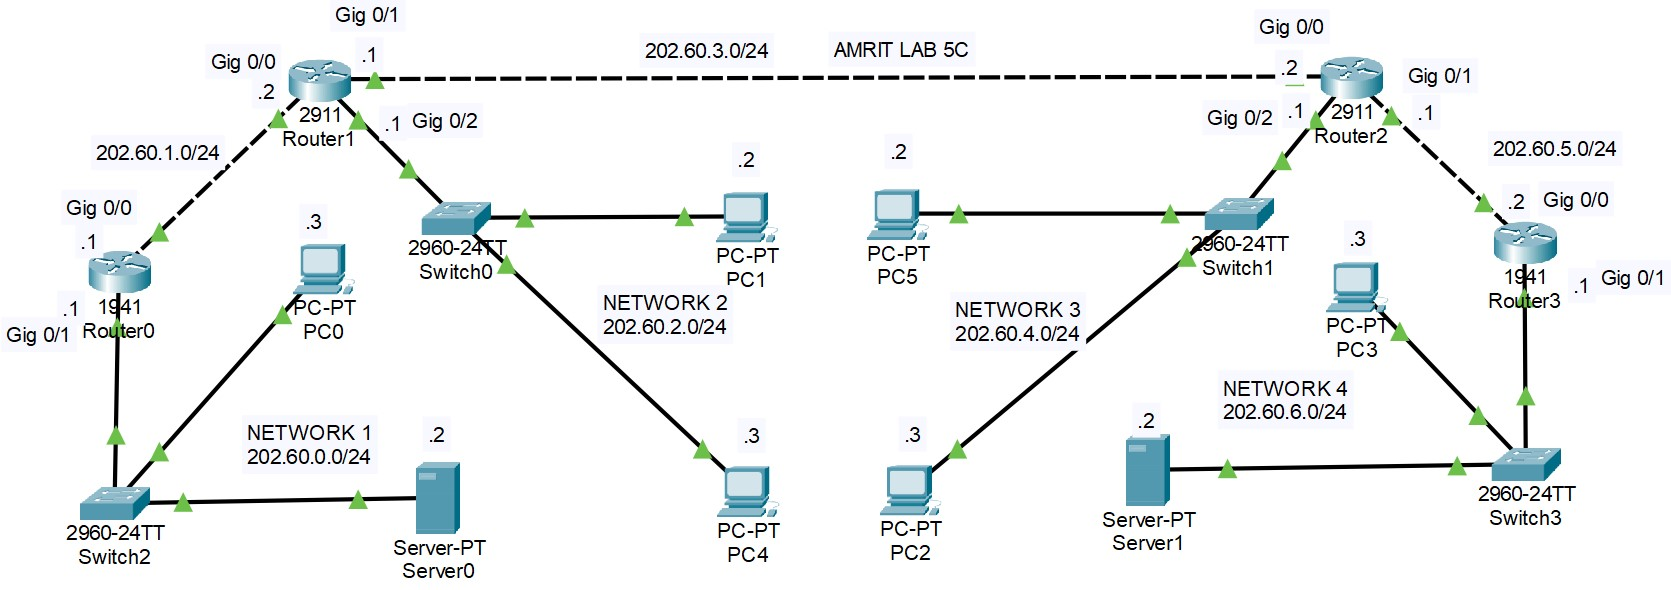
\includegraphics[scale=0.50,cframe=blue 0.5pt 3pt]{Lab5C.jpg}
    \caption{Network topology Lab 5C}
\end{figure}

\begin{enumerate}
    %%%%%%%%%%%%%%%%%%%%%%%%CCCCCCCCCCCCCCCCCCCCCCCCCCCCC11111111111111111111111
    \item \textbf{ Minimize the static route entries by configuring the default route in each Router.}



          \addtocontents{lol}{\protect\subsection*{\HRule \\
                  Activities C: Default Route\\
                  \HRule }}
          \addtocontents{lol}{\protect\subsubsection*{C.1 : Minimizing entries in Routing Table }}
          \CMD{C_Dr0.txt}{Minimize static route entries in Router 0}
          \CMD{C_Dr1.txt}{Minimize static route entries in Router 1}
          \CMD{C_Dr2.txt}{Minimize static route entries in Router 2}
          \CMD{C_Dr3.txt}{Minimize static route entries in Router 3}

          %%%%%%%%%%%%%%%%%%%%%%%%CCCCCCCCCCCCCCCCCCCCCCCCCCCCC22222222222222222222222222
    \item\textbf{  Test the connectivity from PC0, PC1, PC2 and PC3 to each of the given PC and Router using ping command and note down the result.}

          All ping will be Successful among the networks as routers are now able to forward package intended to Unknown destination  to  the next Router in its routing path.
          \begin{enumerate}
              \item \textbf{Ping from PC0 to all after static configuration}
                    \addtocontents{lol}{\protect\subsubsection*{C.2 : Ping from PC0, PC1, PC2,PC3 to all others }}
                    \CMD{SCP0-3.txt}{Ping from PC0 to PC3}

                    \addtocontents{lot}{\protect\subsection*{\HRule \\
                            Activities C: Default Route\\
                            \HRule }}

                    \addtocontents{lot}{\protect\subsubsection*{C.2 : Ping from PC0, PC1, PC2,PC3 to all others }}

                    \begin{table}[H]
                        \centering
                        \arrayrulecolor{black}
                        \begin{tabular}{| m{9em}| m{12em}| m{9em} |}
                            \hline
                            \textbf{Sending Host}                                           & \textbf{Destination} & \textbf{Ping status}                                                     \\
                            \hline
                            {\cellcolor[rgb]{0.333,0.686,1}}                                & PC0                  & {\cellcolor[rgb]{0.365,1,0.741}}                                         \\
                            \hhline{|>{\arrayrulecolor[rgb]{0.333,0.686,1}}->{\arrayrulecolor{black}}->{\arrayrulecolor[rgb]{0.365,1,0.741}}->{\arrayrulecolor{black}}|}
                            {\cellcolor[rgb]{0.333,0.686,1}}                                & Server 0             & {\cellcolor[rgb]{0.365,1,0.741}}                                         \\
                            \hhline{|>{\arrayrulecolor[rgb]{0.333,0.686,1}}->{\arrayrulecolor{black}}->{\arrayrulecolor[rgb]{0.365,1,0.741}}->{\arrayrulecolor{black}}|}
                            {\cellcolor[rgb]{0.333,0.686,1}}                                & Router 0 : 0/1       & {\cellcolor[rgb]{0.365,1,0.741}}                                         \\
                            \hhline{|>{\arrayrulecolor[rgb]{0.333,0.686,1}}->{\arrayrulecolor{black}}->{\arrayrulecolor[rgb]{0.365,1,0.741}}->{\arrayrulecolor{black}}|}
                            {\cellcolor[rgb]{0.333,0.686,1}}                                & Router 0 : 0/0       & {\cellcolor[rgb]{0.365,1,0.741}}                                         \\
                            \hhline{|>{\arrayrulecolor[rgb]{0.333,0.686,1}}->{\arrayrulecolor{black}}->{\arrayrulecolor[rgb]{0.365,1,0.741}}->{\arrayrulecolor{black}}|}
                            {\cellcolor[rgb]{0.333,0.686,1}}                                & Router 1 : 0/0       & {\cellcolor[rgb]{0.365,1,0.741}}                                         \\
                            \hhline{|>{\arrayrulecolor[rgb]{0.333,0.686,1}}->{\arrayrulecolor{black}}->{\arrayrulecolor[rgb]{0.365,1,0.741}}->{\arrayrulecolor{black}}|}
                            {\cellcolor[rgb]{0.333,0.686,1}}                                & Router 1 : 0/1       & {\cellcolor[rgb]{0.365,1,0.741}}                                         \\
                            \hhline{|>{\arrayrulecolor[rgb]{0.333,0.686,1}}->{\arrayrulecolor{black}}->{\arrayrulecolor[rgb]{0.365,1,0.741}}->{\arrayrulecolor{black}}|}
                            {\cellcolor[rgb]{0.333,0.686,1}}                                & Router 1 : 0/2       & {\cellcolor[rgb]{0.365,1,0.741}}                                         \\
                            \hhline{|>{\arrayrulecolor[rgb]{0.333,0.686,1}}->{\arrayrulecolor{black}}->{\arrayrulecolor[rgb]{0.365,1,0.741}}->{\arrayrulecolor{black}}|}
                            {\cellcolor[rgb]{0.333,0.686,1}}                                & PC1                  & {\cellcolor[rgb]{0.365,1,0.741}}                                         \\
                            \hhline{|>{\arrayrulecolor[rgb]{0.333,0.686,1}}->{\arrayrulecolor{black}}->{\arrayrulecolor[rgb]{0.365,1,0.741}}->{\arrayrulecolor{black}}|}
                            {\cellcolor[rgb]{0.333,0.686,1}}                                & Router 2 : 0/0       & {\cellcolor[rgb]{0.365,1,0.741}}                                         \\
                            \hhline{|>{\arrayrulecolor[rgb]{0.333,0.686,1}}->{\arrayrulecolor{black}}->{\arrayrulecolor[rgb]{0.365,1,0.741}}->{\arrayrulecolor{black}}|}
                            {\cellcolor[rgb]{0.333,0.686,1}}                                & Router 2 : 0/2       & {\cellcolor[rgb]{0.365,1,0.741}}                                         \\
                            \hhline{|>{\arrayrulecolor[rgb]{0.333,0.686,1}}->{\arrayrulecolor{black}}->{\arrayrulecolor[rgb]{0.365,1,0.741}}->{\arrayrulecolor{black}}|}
                            {\cellcolor[rgb]{0.333,0.686,1}}                                & PC2                  & {\cellcolor[rgb]{0.365,1,0.741}}                                         \\
                            \hhline{|>{\arrayrulecolor[rgb]{0.333,0.686,1}}->{\arrayrulecolor{black}}->{\arrayrulecolor[rgb]{0.365,1,0.741}}->{\arrayrulecolor{black}}|}
                            {\cellcolor[rgb]{0.333,0.686,1}}                                & Router 2 : 0/1       & {\cellcolor[rgb]{0.365,1,0.741}}                                         \\
                            \hhline{|>{\arrayrulecolor[rgb]{0.333,0.686,1}}->{\arrayrulecolor{black}}->{\arrayrulecolor[rgb]{0.365,1,0.741}}->{\arrayrulecolor{black}}|}
                            {\cellcolor[rgb]{0.333,0.686,1}}                                & Router 3 : 0/0       & {\cellcolor[rgb]{0.365,1,0.741}}                                         \\
                            \hhline{|>{\arrayrulecolor[rgb]{0.333,0.686,1}}->{\arrayrulecolor{black}}->{\arrayrulecolor[rgb]{0.365,1,0.741}}->{\arrayrulecolor{black}}|}
                            {\cellcolor[rgb]{0.333,0.686,1}}                                & Router 3 : 0/1       & {\cellcolor[rgb]{0.365,1,0.741}}                                         \\
                            \hhline{|>{\arrayrulecolor[rgb]{0.333,0.686,1}}->{\arrayrulecolor{black}}->{\arrayrulecolor[rgb]{0.365,1,0.741}}->{\arrayrulecolor{black}}|}
                            {\cellcolor[rgb]{0.333,0.686,1}}                                & PC3                  & {\cellcolor[rgb]{0.365,1,0.741}}                                         \\
                            \hhline{|>{\arrayrulecolor[rgb]{0.333,0.686,1}}->{\arrayrulecolor{black}}->{\arrayrulecolor[rgb]{0.365,1,0.741}}->{\arrayrulecolor{black}}|}
                            \multirow{-16}{*}{{\cellcolor[rgb]{0.333,0.686,1}}\textbf{PC0}} & Server 1             & \multirow{-16}{*}{{\cellcolor[rgb]{0.365,1,0.741}} \textbf{Successful}~} \\
                            \hline
                        \end{tabular}
                        \caption{Ping from PC0 to all Routers,PCs and Servers }
                    \end{table}

              \item \textbf{Ping from PC1 to all after static configuration}
                    \CMD{SCP1-3.txt}{Ping from PC1 to PC3}
                    \begin{table}[H]
                        \centering
                        \arrayrulecolor{black}
                        \begin{tabular}{| m{9em}| m{12em}| m{9em} |}
                            \hline
                            \textbf{Sending Host}                                           & \textbf{Destination} & \textbf{Ping status}                                                     \\
                            \hline
                            {\cellcolor[rgb]{0.333,0.686,1}}                                & PC0                  & {\cellcolor[rgb]{0.365,1,0.741}}                                         \\
                            \hhline{|>{\arrayrulecolor[rgb]{0.333,0.686,1}}->{\arrayrulecolor{black}}->{\arrayrulecolor[rgb]{0.365,1,0.741}}->{\arrayrulecolor{black}}|}
                            {\cellcolor[rgb]{0.333,0.686,1}}                                & Server 0             & {\cellcolor[rgb]{0.365,1,0.741}}                                         \\
                            \hhline{|>{\arrayrulecolor[rgb]{0.333,0.686,1}}->{\arrayrulecolor{black}}->{\arrayrulecolor[rgb]{0.365,1,0.741}}->{\arrayrulecolor{black}}|}
                            {\cellcolor[rgb]{0.333,0.686,1}}                                & Router 0 : 0/1       & {\cellcolor[rgb]{0.365,1,0.741}}                                         \\
                            \hhline{|>{\arrayrulecolor[rgb]{0.333,0.686,1}}->{\arrayrulecolor{black}}->{\arrayrulecolor[rgb]{0.365,1,0.741}}->{\arrayrulecolor{black}}|}
                            {\cellcolor[rgb]{0.333,0.686,1}}                                & Router 0 : 0/0       & {\cellcolor[rgb]{0.365,1,0.741}}                                         \\
                            \hhline{|>{\arrayrulecolor[rgb]{0.333,0.686,1}}->{\arrayrulecolor{black}}->{\arrayrulecolor[rgb]{0.365,1,0.741}}->{\arrayrulecolor{black}}|}
                            {\cellcolor[rgb]{0.333,0.686,1}}                                & Router 1 : 0/0       & {\cellcolor[rgb]{0.365,1,0.741}}                                         \\
                            \hhline{|>{\arrayrulecolor[rgb]{0.333,0.686,1}}->{\arrayrulecolor{black}}->{\arrayrulecolor[rgb]{0.365,1,0.741}}->{\arrayrulecolor{black}}|}
                            {\cellcolor[rgb]{0.333,0.686,1}}                                & Router 1 : 0/1       & {\cellcolor[rgb]{0.365,1,0.741}}                                         \\
                            \hhline{|>{\arrayrulecolor[rgb]{0.333,0.686,1}}->{\arrayrulecolor{black}}->{\arrayrulecolor[rgb]{0.365,1,0.741}}->{\arrayrulecolor{black}}|}
                            {\cellcolor[rgb]{0.333,0.686,1}}                                & Router 1 : 0/2       & {\cellcolor[rgb]{0.365,1,0.741}}                                         \\
                            \hhline{|>{\arrayrulecolor[rgb]{0.333,0.686,1}}->{\arrayrulecolor{black}}->{\arrayrulecolor[rgb]{0.365,1,0.741}}->{\arrayrulecolor{black}}|}
                            {\cellcolor[rgb]{0.333,0.686,1}}                                & PC1                  & {\cellcolor[rgb]{0.365,1,0.741}}                                         \\
                            \hhline{|>{\arrayrulecolor[rgb]{0.333,0.686,1}}->{\arrayrulecolor{black}}->{\arrayrulecolor[rgb]{0.365,1,0.741}}->{\arrayrulecolor{black}}|}
                            {\cellcolor[rgb]{0.333,0.686,1}}                                & Router 2 : 0/0       & {\cellcolor[rgb]{0.365,1,0.741}}                                         \\
                            \hhline{|>{\arrayrulecolor[rgb]{0.333,0.686,1}}->{\arrayrulecolor{black}}->{\arrayrulecolor[rgb]{0.365,1,0.741}}->{\arrayrulecolor{black}}|}
                            {\cellcolor[rgb]{0.333,0.686,1}}                                & Router 2 : 0/2       & {\cellcolor[rgb]{0.365,1,0.741}}                                         \\
                            \hhline{|>{\arrayrulecolor[rgb]{0.333,0.686,1}}->{\arrayrulecolor{black}}->{\arrayrulecolor[rgb]{0.365,1,0.741}}->{\arrayrulecolor{black}}|}
                            {\cellcolor[rgb]{0.333,0.686,1}}                                & PC2                  & {\cellcolor[rgb]{0.365,1,0.741}}                                         \\
                            \hhline{|>{\arrayrulecolor[rgb]{0.333,0.686,1}}->{\arrayrulecolor{black}}->{\arrayrulecolor[rgb]{0.365,1,0.741}}->{\arrayrulecolor{black}}|}
                            {\cellcolor[rgb]{0.333,0.686,1}}                                & Router 2 : 0/1       & {\cellcolor[rgb]{0.365,1,0.741}}                                         \\
                            \hhline{|>{\arrayrulecolor[rgb]{0.333,0.686,1}}->{\arrayrulecolor{black}}->{\arrayrulecolor[rgb]{0.365,1,0.741}}->{\arrayrulecolor{black}}|}
                            {\cellcolor[rgb]{0.333,0.686,1}}                                & Router 3 : 0/0       & {\cellcolor[rgb]{0.365,1,0.741}}                                         \\
                            \hhline{|>{\arrayrulecolor[rgb]{0.333,0.686,1}}->{\arrayrulecolor{black}}->{\arrayrulecolor[rgb]{0.365,1,0.741}}->{\arrayrulecolor{black}}|}
                            {\cellcolor[rgb]{0.333,0.686,1}}                                & Router 3 : 0/1       & {\cellcolor[rgb]{0.365,1,0.741}}                                         \\
                            \hhline{|>{\arrayrulecolor[rgb]{0.333,0.686,1}}->{\arrayrulecolor{black}}->{\arrayrulecolor[rgb]{0.365,1,0.741}}->{\arrayrulecolor{black}}|}
                            {\cellcolor[rgb]{0.333,0.686,1}}                                & PC3                  & {\cellcolor[rgb]{0.365,1,0.741}}                                         \\
                            \hhline{|>{\arrayrulecolor[rgb]{0.333,0.686,1}}->{\arrayrulecolor{black}}->{\arrayrulecolor[rgb]{0.365,1,0.741}}->{\arrayrulecolor{black}}|}
                            \multirow{-16}{*}{{\cellcolor[rgb]{0.333,0.686,1}}\textbf{PC1}} & Server 1             & \multirow{-16}{*}{{\cellcolor[rgb]{0.365,1,0.741}} \textbf{Successful}~} \\
                            \hline
                        \end{tabular}
                        \caption{Ping from PC1 to all Routers,PCs and Servers }
                    \end{table}

              \item \textbf{Ping from PC2 to all after static configuration}
                    \CMD{SCP2-r01.txt}{Ping from PC2 to Router 0 : 0/1}
                    \begin{table}[H]
                        \centering
                        \arrayrulecolor{black}
                        \begin{tabular}{| m{9em}| m{12em}| m{9em} |}
                            \hline
                            \textbf{Sending Host}                                           & \textbf{Destination} & \textbf{Ping status}                                                     \\
                            \hline
                            {\cellcolor[rgb]{0.333,0.686,1}}                                & PC0                  & {\cellcolor[rgb]{0.365,1,0.741}}                                         \\
                            \hhline{|>{\arrayrulecolor[rgb]{0.333,0.686,1}}->{\arrayrulecolor{black}}->{\arrayrulecolor[rgb]{0.365,1,0.741}}->{\arrayrulecolor{black}}|}
                            {\cellcolor[rgb]{0.333,0.686,1}}                                & Server 0             & {\cellcolor[rgb]{0.365,1,0.741}}                                         \\
                            \hhline{|>{\arrayrulecolor[rgb]{0.333,0.686,1}}->{\arrayrulecolor{black}}->{\arrayrulecolor[rgb]{0.365,1,0.741}}->{\arrayrulecolor{black}}|}
                            {\cellcolor[rgb]{0.333,0.686,1}}                                & Router 0 : 0/1       & {\cellcolor[rgb]{0.365,1,0.741}}                                         \\
                            \hhline{|>{\arrayrulecolor[rgb]{0.333,0.686,1}}->{\arrayrulecolor{black}}->{\arrayrulecolor[rgb]{0.365,1,0.741}}->{\arrayrulecolor{black}}|}
                            {\cellcolor[rgb]{0.333,0.686,1}}                                & Router 0 : 0/0       & {\cellcolor[rgb]{0.365,1,0.741}}                                         \\
                            \hhline{|>{\arrayrulecolor[rgb]{0.333,0.686,1}}->{\arrayrulecolor{black}}->{\arrayrulecolor[rgb]{0.365,1,0.741}}->{\arrayrulecolor{black}}|}
                            {\cellcolor[rgb]{0.333,0.686,1}}                                & Router 1 : 0/0       & {\cellcolor[rgb]{0.365,1,0.741}}                                         \\
                            \hhline{|>{\arrayrulecolor[rgb]{0.333,0.686,1}}->{\arrayrulecolor{black}}->{\arrayrulecolor[rgb]{0.365,1,0.741}}->{\arrayrulecolor{black}}|}
                            {\cellcolor[rgb]{0.333,0.686,1}}                                & Router 1 : 0/1       & {\cellcolor[rgb]{0.365,1,0.741}}                                         \\
                            \hhline{|>{\arrayrulecolor[rgb]{0.333,0.686,1}}->{\arrayrulecolor{black}}->{\arrayrulecolor[rgb]{0.365,1,0.741}}->{\arrayrulecolor{black}}|}
                            {\cellcolor[rgb]{0.333,0.686,1}}                                & Router 1 : 0/2       & {\cellcolor[rgb]{0.365,1,0.741}}                                         \\
                            \hhline{|>{\arrayrulecolor[rgb]{0.333,0.686,1}}->{\arrayrulecolor{black}}->{\arrayrulecolor[rgb]{0.365,1,0.741}}->{\arrayrulecolor{black}}|}
                            {\cellcolor[rgb]{0.333,0.686,1}}                                & PC1                  & {\cellcolor[rgb]{0.365,1,0.741}}                                         \\
                            \hhline{|>{\arrayrulecolor[rgb]{0.333,0.686,1}}->{\arrayrulecolor{black}}->{\arrayrulecolor[rgb]{0.365,1,0.741}}->{\arrayrulecolor{black}}|}
                            {\cellcolor[rgb]{0.333,0.686,1}}                                & Router 2 : 0/0       & {\cellcolor[rgb]{0.365,1,0.741}}                                         \\
                            \hhline{|>{\arrayrulecolor[rgb]{0.333,0.686,1}}->{\arrayrulecolor{black}}->{\arrayrulecolor[rgb]{0.365,1,0.741}}->{\arrayrulecolor{black}}|}
                            {\cellcolor[rgb]{0.333,0.686,1}}                                & Router 2 : 0/2       & {\cellcolor[rgb]{0.365,1,0.741}}                                         \\
                            \hhline{|>{\arrayrulecolor[rgb]{0.333,0.686,1}}->{\arrayrulecolor{black}}->{\arrayrulecolor[rgb]{0.365,1,0.741}}->{\arrayrulecolor{black}}|}
                            {\cellcolor[rgb]{0.333,0.686,1}}                                & PC2                  & {\cellcolor[rgb]{0.365,1,0.741}}                                         \\
                            \hhline{|>{\arrayrulecolor[rgb]{0.333,0.686,1}}->{\arrayrulecolor{black}}->{\arrayrulecolor[rgb]{0.365,1,0.741}}->{\arrayrulecolor{black}}|}
                            {\cellcolor[rgb]{0.333,0.686,1}}                                & Router 2 : 0/1       & {\cellcolor[rgb]{0.365,1,0.741}}                                         \\
                            \hhline{|>{\arrayrulecolor[rgb]{0.333,0.686,1}}->{\arrayrulecolor{black}}->{\arrayrulecolor[rgb]{0.365,1,0.741}}->{\arrayrulecolor{black}}|}
                            {\cellcolor[rgb]{0.333,0.686,1}}                                & Router 3 : 0/0       & {\cellcolor[rgb]{0.365,1,0.741}}                                         \\
                            \hhline{|>{\arrayrulecolor[rgb]{0.333,0.686,1}}->{\arrayrulecolor{black}}->{\arrayrulecolor[rgb]{0.365,1,0.741}}->{\arrayrulecolor{black}}|}
                            {\cellcolor[rgb]{0.333,0.686,1}}                                & Router 3 : 0/1       & {\cellcolor[rgb]{0.365,1,0.741}}                                         \\
                            \hhline{|>{\arrayrulecolor[rgb]{0.333,0.686,1}}->{\arrayrulecolor{black}}->{\arrayrulecolor[rgb]{0.365,1,0.741}}->{\arrayrulecolor{black}}|}
                            {\cellcolor[rgb]{0.333,0.686,1}}                                & PC3                  & {\cellcolor[rgb]{0.365,1,0.741}}                                         \\
                            \hhline{|>{\arrayrulecolor[rgb]{0.333,0.686,1}}->{\arrayrulecolor{black}}->{\arrayrulecolor[rgb]{0.365,1,0.741}}->{\arrayrulecolor{black}}|}
                            \multirow{-16}{*}{{\cellcolor[rgb]{0.333,0.686,1}}\textbf{PC2}} & Server 1             & \multirow{-16}{*}{{\cellcolor[rgb]{0.365,1,0.741}} \textbf{Successful}~} \\
                            \hline
                        \end{tabular}
                        \caption{Ping from PC2 to all Routers,PCs and Servers }
                    \end{table}

              \item \textbf{Ping from PC3 to all after static configuration}
                    \CMD{SCP3-1.txt}{Ping from PC3 to PC1}

                    \begin{table}[H]
                        \centering
                        \arrayrulecolor{black}
                        \begin{tabular}{| m{9em}| m{12em}| m{9em} |}
                            \hline
                            \textbf{Sending Host}                                           & \textbf{Destination} & \textbf{Ping status}                                                     \\
                            \hline
                            {\cellcolor[rgb]{0.333,0.686,1}}                                & PC0                  & {\cellcolor[rgb]{0.365,1,0.741}}                                         \\
                            \hhline{|>{\arrayrulecolor[rgb]{0.333,0.686,1}}->{\arrayrulecolor{black}}->{\arrayrulecolor[rgb]{0.365,1,0.741}}->{\arrayrulecolor{black}}|}
                            {\cellcolor[rgb]{0.333,0.686,1}}                                & Server 0             & {\cellcolor[rgb]{0.365,1,0.741}}                                         \\
                            \hhline{|>{\arrayrulecolor[rgb]{0.333,0.686,1}}->{\arrayrulecolor{black}}->{\arrayrulecolor[rgb]{0.365,1,0.741}}->{\arrayrulecolor{black}}|}
                            {\cellcolor[rgb]{0.333,0.686,1}}                                & Router 0 : 0/1       & {\cellcolor[rgb]{0.365,1,0.741}}                                         \\
                            \hhline{|>{\arrayrulecolor[rgb]{0.333,0.686,1}}->{\arrayrulecolor{black}}->{\arrayrulecolor[rgb]{0.365,1,0.741}}->{\arrayrulecolor{black}}|}
                            {\cellcolor[rgb]{0.333,0.686,1}}                                & Router 0 : 0/0       & {\cellcolor[rgb]{0.365,1,0.741}}                                         \\
                            \hhline{|>{\arrayrulecolor[rgb]{0.333,0.686,1}}->{\arrayrulecolor{black}}->{\arrayrulecolor[rgb]{0.365,1,0.741}}->{\arrayrulecolor{black}}|}
                            {\cellcolor[rgb]{0.333,0.686,1}}                                & Router 1 : 0/0       & {\cellcolor[rgb]{0.365,1,0.741}}                                         \\
                            \hhline{|>{\arrayrulecolor[rgb]{0.333,0.686,1}}->{\arrayrulecolor{black}}->{\arrayrulecolor[rgb]{0.365,1,0.741}}->{\arrayrulecolor{black}}|}
                            {\cellcolor[rgb]{0.333,0.686,1}}                                & Router 1 : 0/1       & {\cellcolor[rgb]{0.365,1,0.741}}                                         \\
                            \hhline{|>{\arrayrulecolor[rgb]{0.333,0.686,1}}->{\arrayrulecolor{black}}->{\arrayrulecolor[rgb]{0.365,1,0.741}}->{\arrayrulecolor{black}}|}
                            {\cellcolor[rgb]{0.333,0.686,1}}                                & Router 1 : 0/2       & {\cellcolor[rgb]{0.365,1,0.741}}                                         \\
                            \hhline{|>{\arrayrulecolor[rgb]{0.333,0.686,1}}->{\arrayrulecolor{black}}->{\arrayrulecolor[rgb]{0.365,1,0.741}}->{\arrayrulecolor{black}}|}
                            {\cellcolor[rgb]{0.333,0.686,1}}                                & PC1                  & {\cellcolor[rgb]{0.365,1,0.741}}                                         \\
                            \hhline{|>{\arrayrulecolor[rgb]{0.333,0.686,1}}->{\arrayrulecolor{black}}->{\arrayrulecolor[rgb]{0.365,1,0.741}}->{\arrayrulecolor{black}}|}
                            {\cellcolor[rgb]{0.333,0.686,1}}                                & Router 2 : 0/0       & {\cellcolor[rgb]{0.365,1,0.741}}                                         \\
                            \hhline{|>{\arrayrulecolor[rgb]{0.333,0.686,1}}->{\arrayrulecolor{black}}->{\arrayrulecolor[rgb]{0.365,1,0.741}}->{\arrayrulecolor{black}}|}
                            {\cellcolor[rgb]{0.333,0.686,1}}                                & Router 2 : 0/2       & {\cellcolor[rgb]{0.365,1,0.741}}                                         \\
                            \hhline{|>{\arrayrulecolor[rgb]{0.333,0.686,1}}->{\arrayrulecolor{black}}->{\arrayrulecolor[rgb]{0.365,1,0.741}}->{\arrayrulecolor{black}}|}
                            {\cellcolor[rgb]{0.333,0.686,1}}                                & PC2                  & {\cellcolor[rgb]{0.365,1,0.741}}                                         \\
                            \hhline{|>{\arrayrulecolor[rgb]{0.333,0.686,1}}->{\arrayrulecolor{black}}->{\arrayrulecolor[rgb]{0.365,1,0.741}}->{\arrayrulecolor{black}}|}
                            {\cellcolor[rgb]{0.333,0.686,1}}                                & Router 2 : 0/1       & {\cellcolor[rgb]{0.365,1,0.741}}                                         \\
                            \hhline{|>{\arrayrulecolor[rgb]{0.333,0.686,1}}->{\arrayrulecolor{black}}->{\arrayrulecolor[rgb]{0.365,1,0.741}}->{\arrayrulecolor{black}}|}
                            {\cellcolor[rgb]{0.333,0.686,1}}                                & Router 3 : 0/0       & {\cellcolor[rgb]{0.365,1,0.741}}                                         \\
                            \hhline{|>{\arrayrulecolor[rgb]{0.333,0.686,1}}->{\arrayrulecolor{black}}->{\arrayrulecolor[rgb]{0.365,1,0.741}}->{\arrayrulecolor{black}}|}
                            {\cellcolor[rgb]{0.333,0.686,1}}                                & Router 3 : 0/1       & {\cellcolor[rgb]{0.365,1,0.741}}                                         \\
                            \hhline{|>{\arrayrulecolor[rgb]{0.333,0.686,1}}->{\arrayrulecolor{black}}->{\arrayrulecolor[rgb]{0.365,1,0.741}}->{\arrayrulecolor{black}}|}
                            {\cellcolor[rgb]{0.333,0.686,1}}                                & PC3                  & {\cellcolor[rgb]{0.365,1,0.741}}                                         \\
                            \hhline{|>{\arrayrulecolor[rgb]{0.333,0.686,1}}->{\arrayrulecolor{black}}->{\arrayrulecolor[rgb]{0.365,1,0.741}}->{\arrayrulecolor{black}}|}
                            \multirow{-16}{*}{{\cellcolor[rgb]{0.333,0.686,1}}\textbf{PC3}} & Server 1             & \multirow{-16}{*}{{\cellcolor[rgb]{0.365,1,0.741}} \textbf{Successful}~} \\
                            \hline
                        \end{tabular}
                        \caption{Ping from PC3 to all Routers,PCs and Servers }
                    \end{table}




          \end{enumerate}

          %%%%%%%%%%%%%%%%%%%%%%%%CCCCCCCCCCCCCCCCCCCCCCCCCCCCC33333333333333333333333
    \item\textbf{  Observe the output of \textit{show ip route} in each Router and note down the result.}

          \addtocontents{lol}{\protect\subsubsection*{C.3 : Routing Table after Default Route Configuration}}

          \CMD{C_Showip0.txt}{\textit{show ip route} Router 0 }
          \CMD{C_Showip1.txt}{\textit{show ip route} Router 1 }
          \CMD{C_Showip2.txt}{\textit{show ip route} Router 2 }
          \CMD{C_Showip3.txt}{\textit{show ip route} Router 3 }

          %%%%%%%%%%%%%%%%%%%%%%%%CCCCCCCCCCCCCCCCCCCCCCCCCCCCC444444444444444444444
    \item\textbf{ Compare the output of \textit{show ip route} command used in question 18 of activity B and question 3 of activity C.}

          Here we used our understanding and knowledge of default route to our advantage to reduce entries in Routing Table. To be clear  in Router 0 all the outgoing traffic is forwarded to Router 1 and default route is configured accordingly thus reducing the entries from 4 to 1 comparing to Activity B.18.Similarly  in Router 2 Static route is configured for Network 4 (Router 3) and all other outgoing package if forwarded to Router 1 using Default Route Configuration hence reducing entries from 4 to 2.


          %%%%%%%%%%%%%%%%%%%%%%%%CCCCCCCCCCCCCCCCCCCCCCCCCCCCC555555555555555555555555555
    \item\textbf{  The hostname of each Router should be as your LastName\_0, LastName\_1 and so on.}

          Already Edited to required format.


\end{enumerate}


\section{Conclusion:}

In this Lab we familiarize ourselves with Static and Default Route .
In activity A we performed default  route configuration to have insight of topic and compared the ping performed before and after setting Default Route. In Activity B we used Static Route and configure each Router for each available network and also compared the result of Ping Operation Before and after configuring Static Route. in the same Activity we also compared the Routing Table and found that in each routers 4 additional  entries are added as Static Route. Similarly in Activity C we try to minimize those entries in Routing Table using Knowledge of Default Route and we were successful . In the same Activity we performed the ping operation after setting the default routes and deleting unwanted entries from Routing Tables of all Routers. We also performed Telnet ,configured hostname and password for various purposes.

\end{document}